\documentclass[twoside]{book}

% Packages required by doxygen
\usepackage{fixltx2e}
\usepackage{calc}
\usepackage{doxygen}
\usepackage[export]{adjustbox} % also loads graphicx
\usepackage{graphicx}
\usepackage[utf8]{inputenc}
\usepackage{makeidx}
\usepackage{multicol}
\usepackage{multirow}
\PassOptionsToPackage{warn}{textcomp}
\usepackage{textcomp}
\usepackage[nointegrals]{wasysym}
\usepackage[table]{xcolor}

% Font selection
\usepackage[T1]{fontenc}
\usepackage[scaled=.90]{helvet}
\usepackage{courier}
\usepackage{amssymb}
\usepackage{sectsty}
\renewcommand{\familydefault}{\sfdefault}
\allsectionsfont{%
  \fontseries{bc}\selectfont%
  \color{darkgray}%
}
\renewcommand{\DoxyLabelFont}{%
  \fontseries{bc}\selectfont%
  \color{darkgray}%
}
\newcommand{\+}{\discretionary{\mbox{\scriptsize$\hookleftarrow$}}{}{}}

% Page & text layout
\usepackage{geometry}
\geometry{%
  a4paper,%
  top=2.5cm,%
  bottom=2.5cm,%
  left=2.5cm,%
  right=2.5cm%
}
\tolerance=750
\hfuzz=15pt
\hbadness=750
\setlength{\emergencystretch}{15pt}
\setlength{\parindent}{0cm}
\setlength{\parskip}{3ex plus 2ex minus 2ex}
\makeatletter
\renewcommand{\paragraph}{%
  \@startsection{paragraph}{4}{0ex}{-1.0ex}{1.0ex}{%
    \normalfont\normalsize\bfseries\SS@parafont%
  }%
}
\renewcommand{\subparagraph}{%
  \@startsection{subparagraph}{5}{0ex}{-1.0ex}{1.0ex}{%
    \normalfont\normalsize\bfseries\SS@subparafont%
  }%
}
\makeatother

% Headers & footers
\usepackage{fancyhdr}
\pagestyle{fancyplain}
\fancyhead[LE]{\fancyplain{}{\bfseries\thepage}}
\fancyhead[CE]{\fancyplain{}{}}
\fancyhead[RE]{\fancyplain{}{\bfseries\leftmark}}
\fancyhead[LO]{\fancyplain{}{\bfseries\rightmark}}
\fancyhead[CO]{\fancyplain{}{}}
\fancyhead[RO]{\fancyplain{}{\bfseries\thepage}}
\fancyfoot[LE]{\fancyplain{}{}}
\fancyfoot[CE]{\fancyplain{}{}}
\fancyfoot[RE]{\fancyplain{}{\bfseries\scriptsize Generated by Doxygen }}
\fancyfoot[LO]{\fancyplain{}{\bfseries\scriptsize Generated by Doxygen }}
\fancyfoot[CO]{\fancyplain{}{}}
\fancyfoot[RO]{\fancyplain{}{}}
\renewcommand{\footrulewidth}{0.4pt}
\renewcommand{\chaptermark}[1]{%
  \markboth{#1}{}%
}
\renewcommand{\sectionmark}[1]{%
  \markright{\thesection\ #1}%
}

% Indices & bibliography
\usepackage{natbib}
\usepackage[titles]{tocloft}
\setcounter{tocdepth}{3}
\setcounter{secnumdepth}{5}
\makeindex

% Hyperlinks (required, but should be loaded last)
\usepackage{ifpdf}
\ifpdf
  \usepackage[pdftex,pagebackref=true]{hyperref}
\else
  \usepackage[ps2pdf,pagebackref=true]{hyperref}
\fi
\hypersetup{%
  colorlinks=true,%
  linkcolor=blue,%
  citecolor=blue,%
  unicode%
}

% Custom commands
\newcommand{\clearemptydoublepage}{%
  \newpage{\pagestyle{empty}\cleardoublepage}%
}

\usepackage{caption}
\captionsetup{labelsep=space,justification=centering,font={bf},singlelinecheck=off,skip=4pt,position=top}

%===== C O N T E N T S =====

\begin{document}

% Titlepage & ToC
\hypersetup{pageanchor=false,
             bookmarksnumbered=true,
             pdfencoding=unicode
            }
\pagenumbering{roman}
\begin{titlepage}
\vspace*{7cm}
\begin{center}%
{\Large Car Game \\[1ex]\large 1.\+0.\+0 }\\
\vspace*{1cm}
{\large Generated by Doxygen 1.8.11}\\
\end{center}
\end{titlepage}
\clearemptydoublepage
\tableofcontents
\clearemptydoublepage
\pagenumbering{arabic}
\hypersetup{pageanchor=true}

%--- Begin generated contents ---
\chapter{Hierarchical Index}
\section{Class Hierarchy}
This inheritance list is sorted roughly, but not completely, alphabetically\+:\begin{DoxyCompactList}
\item \contentsline{section}{Audio\+Loader}{\pageref{class_audio_loader}}{}
\item Circle\+Shape\begin{DoxyCompactList}
\item \contentsline{section}{Circle}{\pageref{class_circle}}{}
\begin{DoxyCompactList}
\item \contentsline{section}{Sphere\+Trigger}{\pageref{class_sphere_trigger}}{}
\item \contentsline{section}{Tire}{\pageref{class_tire}}{}
\end{DoxyCompactList}
\end{DoxyCompactList}
\item \contentsline{section}{Collision}{\pageref{class_collision}}{}
\item Drawable\begin{DoxyCompactList}
\item \contentsline{section}{Game}{\pageref{class_game}}{}
\end{DoxyCompactList}
\item \contentsline{section}{Font\+Loader}{\pageref{class_font_loader}}{}
\item \contentsline{section}{Physics}{\pageref{class_physics}}{}
\item Rectangle\+Shape\begin{DoxyCompactList}
\item \contentsline{section}{Rectangle}{\pageref{class_rectangle}}{}
\begin{DoxyCompactList}
\item \contentsline{section}{Checkpoint}{\pageref{class_checkpoint}}{}
\item \contentsline{section}{Player}{\pageref{class_player}}{}
\item \contentsline{section}{Rectangle\+Trigger}{\pageref{class_rectangle_trigger}}{}
\item \contentsline{section}{Static\+Car}{\pageref{class_static_car}}{}
\item \contentsline{section}{Wall}{\pageref{class_wall}}{}
\end{DoxyCompactList}
\end{DoxyCompactList}
\item Sprite\begin{DoxyCompactList}
\item \contentsline{section}{Image}{\pageref{class_image}}{}
\end{DoxyCompactList}
\item Text\begin{DoxyCompactList}
\item \contentsline{section}{Simple\+Text}{\pageref{class_simple_text}}{}
\end{DoxyCompactList}
\item \contentsline{section}{Texture\+Loader}{\pageref{class_texture_loader}}{}
\item \contentsline{section}{Vector\+Maths}{\pageref{class_vector_maths}}{}
\item View\begin{DoxyCompactList}
\item \contentsline{section}{View}{\pageref{class_view}}{}
\end{DoxyCompactList}
\end{DoxyCompactList}

\chapter{Class Index}
\section{Class List}
Here are the classes, structs, unions and interfaces with brief descriptions\+:\begin{DoxyCompactList}
\item\contentsline{section}{\hyperlink{class_audio_loader}{Audio\+Loader} \\*This class is used to manage audio }{\pageref{class_audio_loader}}{}
\item\contentsline{section}{\hyperlink{class_checkpoint}{Checkpoint} \\*This class is used to do create a simple checkpoint }{\pageref{class_checkpoint}}{}
\item\contentsline{section}{\hyperlink{class_circle}{Circle} \\*This class is used to create an abstract base class of the circle }{\pageref{class_circle}}{}
\item\contentsline{section}{\hyperlink{class_collision}{Collision} \\*This class is used to do collision tests }{\pageref{class_collision}}{}
\item\contentsline{section}{\hyperlink{class_font_loader}{Font\+Loader} \\*This class is used to manage fonts }{\pageref{class_font_loader}}{}
\item\contentsline{section}{\hyperlink{class_game}{Game} \\*This class is used to create a game window }{\pageref{class_game}}{}
\item\contentsline{section}{\hyperlink{class_image}{Image} \\*This class is used to construct an image }{\pageref{class_image}}{}
\item\contentsline{section}{\hyperlink{class_physics}{Physics} \\*This class is used to create a simulation of movement }{\pageref{class_physics}}{}
\item\contentsline{section}{\hyperlink{class_player}{Player} \\*This class is used to create and control a player }{\pageref{class_player}}{}
\item\contentsline{section}{\hyperlink{class_rectangle}{Rectangle} \\*This class is used to create an abstract base class of the rectangle }{\pageref{class_rectangle}}{}
\item\contentsline{section}{\hyperlink{class_rectangle_trigger}{Rectangle\+Trigger} \\*This class is used to create a trigger }{\pageref{class_rectangle_trigger}}{}
\item\contentsline{section}{\hyperlink{class_simple_text}{Simple\+Text} \\*This class is used to create a simple text on the screen }{\pageref{class_simple_text}}{}
\item\contentsline{section}{\hyperlink{class_sphere_trigger}{Sphere\+Trigger} \\*This class is used to create a trigger }{\pageref{class_sphere_trigger}}{}
\item\contentsline{section}{\hyperlink{class_static_car}{Static\+Car} \\*This class is used to create immovable cars }{\pageref{class_static_car}}{}
\item\contentsline{section}{\hyperlink{class_texture_loader}{Texture\+Loader} \\*This class is used to manage textures }{\pageref{class_texture_loader}}{}
\item\contentsline{section}{\hyperlink{class_tire}{Tire} \\*This class is used to construct a tire }{\pageref{class_tire}}{}
\item\contentsline{section}{\hyperlink{class_vector_maths}{Vector\+Maths} \\*This class is used to do simple vector calculations }{\pageref{class_vector_maths}}{}
\item\contentsline{section}{\hyperlink{class_view}{View} \\*This class is used to manage a scene }{\pageref{class_view}}{}
\item\contentsline{section}{\hyperlink{class_wall}{Wall} \\*This class is used to construct a wall }{\pageref{class_wall}}{}
\end{DoxyCompactList}

\chapter{File Index}
\section{File List}
Here is a list of all files with brief descriptions\+:\begin{DoxyCompactList}
\item\contentsline{section}{include/\hyperlink{audio_loader_8h}{audio\+Loader.\+h} }{\pageref{audio_loader_8h}}{}
\item\contentsline{section}{include/\hyperlink{checkpoint_8h}{checkpoint.\+h} }{\pageref{checkpoint_8h}}{}
\item\contentsline{section}{include/\hyperlink{circle_8h}{circle.\+h} }{\pageref{circle_8h}}{}
\item\contentsline{section}{include/\hyperlink{collision_8h}{collision.\+h} }{\pageref{collision_8h}}{}
\item\contentsline{section}{include/\hyperlink{font_loader_8h}{font\+Loader.\+h} }{\pageref{font_loader_8h}}{}
\item\contentsline{section}{include/\hyperlink{game_8h}{game.\+h} }{\pageref{game_8h}}{}
\item\contentsline{section}{include/\hyperlink{image_8h}{image.\+h} }{\pageref{image_8h}}{}
\item\contentsline{section}{include/\hyperlink{physics_8h}{physics.\+h} }{\pageref{physics_8h}}{}
\item\contentsline{section}{include/\hyperlink{player_8h}{player.\+h} }{\pageref{player_8h}}{}
\item\contentsline{section}{include/\hyperlink{rectangle_8h}{rectangle.\+h} }{\pageref{rectangle_8h}}{}
\item\contentsline{section}{include/\hyperlink{rectangle_trigger_8h}{rectangle\+Trigger.\+h} }{\pageref{rectangle_trigger_8h}}{}
\item\contentsline{section}{include/\hyperlink{simple_text_8h}{simple\+Text.\+h} }{\pageref{simple_text_8h}}{}
\item\contentsline{section}{include/\hyperlink{sphere_trigger_8h}{sphere\+Trigger.\+h} }{\pageref{sphere_trigger_8h}}{}
\item\contentsline{section}{include/\hyperlink{static_car_8h}{static\+Car.\+h} }{\pageref{static_car_8h}}{}
\item\contentsline{section}{include/\hyperlink{texture_loader_8h}{texture\+Loader.\+h} }{\pageref{texture_loader_8h}}{}
\item\contentsline{section}{include/\hyperlink{tire_8h}{tire.\+h} }{\pageref{tire_8h}}{}
\item\contentsline{section}{include/\hyperlink{vector_maths_8h}{vector\+Maths.\+h} }{\pageref{vector_maths_8h}}{}
\item\contentsline{section}{include/\hyperlink{view_8h}{view.\+h} }{\pageref{view_8h}}{}
\item\contentsline{section}{include/\hyperlink{wall_8h}{wall.\+h} }{\pageref{wall_8h}}{}
\end{DoxyCompactList}

\chapter{Class Documentation}
\hypertarget{class_audio_loader}{}\section{Audio\+Loader Class Reference}
\label{class_audio_loader}\index{Audio\+Loader@{Audio\+Loader}}


This class is used to manage audio.  




{\ttfamily \#include $<$audio\+Loader.\+h$>$}



Collaboration diagram for Audio\+Loader\+:\nopagebreak
\begin{figure}[H]
\begin{center}
\leavevmode
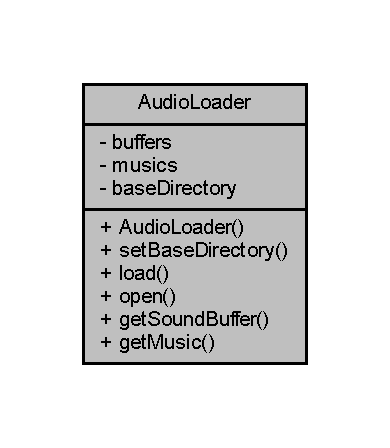
\includegraphics[width=187pt]{class_audio_loader__coll__graph}
\end{center}
\end{figure}
\subsection*{Public Member Functions}
\begin{DoxyCompactItemize}
\item 
\hyperlink{class_audio_loader_a9fe737693de78ab56e73e256cb6474be}{Audio\+Loader} ()
\item 
void \hyperlink{class_audio_loader_a1c836fdf869fa42be7e7d15d52686cf6}{set\+Base\+Directory} (std\+::string dir)
\item 
void \hyperlink{class_audio_loader_ab7182e383a203504a6e8bbd7759088ce}{load} (std\+::vector$<$ std\+::string $>$ file\+Names)
\item 
void \hyperlink{class_audio_loader_a9d8509fa148b954bdac29316e84a26ba}{open} (std\+::vector$<$ std\+::string $>$ file\+Names)
\item 
sf\+::\+Sound\+Buffer \& \hyperlink{class_audio_loader_a8196533d566484ed144f209a41d4ede4}{get\+Sound\+Buffer} (int f\+Index)
\item 
sf\+::\+Music \& \hyperlink{class_audio_loader_adb279e55d3e23c58f8171307fa08180a}{get\+Music} (int f\+Index)
\end{DoxyCompactItemize}
\subsection*{Private Attributes}
\begin{DoxyCompactItemize}
\item 
std\+::vector$<$ sf\+::\+Sound\+Buffer $>$ \hyperlink{class_audio_loader_a000dca4eff031478c1cb39c5d911a5ea}{buffers}
\item 
std\+::array$<$ sf\+::\+Music, 2 $>$ \hyperlink{class_audio_loader_a9e04f423490a0ba4a270751de5dc8226}{musics}
\item 
std\+::string \hyperlink{class_audio_loader_ae6f0dc60b50135750cd8c311296affd3}{base\+Directory}
\end{DoxyCompactItemize}


\subsection{Detailed Description}
This class is used to manage audio. 

\subsection{Constructor \& Destructor Documentation}
\index{Audio\+Loader@{Audio\+Loader}!Audio\+Loader@{Audio\+Loader}}
\index{Audio\+Loader@{Audio\+Loader}!Audio\+Loader@{Audio\+Loader}}
\subsubsection[{\texorpdfstring{Audio\+Loader()}{AudioLoader()}}]{\setlength{\rightskip}{0pt plus 5cm}Audio\+Loader\+::\+Audio\+Loader (
\begin{DoxyParamCaption}
{}
\end{DoxyParamCaption}
)}\hypertarget{class_audio_loader_a9fe737693de78ab56e73e256cb6474be}{}\label{class_audio_loader_a9fe737693de78ab56e73e256cb6474be}
An initializer. 

\subsection{Member Function Documentation}
\index{Audio\+Loader@{Audio\+Loader}!get\+Music@{get\+Music}}
\index{get\+Music@{get\+Music}!Audio\+Loader@{Audio\+Loader}}
\subsubsection[{\texorpdfstring{get\+Music(int f\+Index)}{getMusic(int fIndex)}}]{\setlength{\rightskip}{0pt plus 5cm}sf\+::\+Music\& Audio\+Loader\+::get\+Music (
\begin{DoxyParamCaption}
\item[{int}]{f\+Index}
\end{DoxyParamCaption}
)}\hypertarget{class_audio_loader_adb279e55d3e23c58f8171307fa08180a}{}\label{class_audio_loader_adb279e55d3e23c58f8171307fa08180a}
Returns a music with said index. 
\begin{DoxyParams}{Parameters}
{\em f\+Index} & = Index of the font. \\
\hline
\end{DoxyParams}
\begin{DoxyReturn}{Returns}
$\ast$it = Retruns pointer to the music with matching index. 
\end{DoxyReturn}
\index{Audio\+Loader@{Audio\+Loader}!get\+Sound\+Buffer@{get\+Sound\+Buffer}}
\index{get\+Sound\+Buffer@{get\+Sound\+Buffer}!Audio\+Loader@{Audio\+Loader}}
\subsubsection[{\texorpdfstring{get\+Sound\+Buffer(int f\+Index)}{getSoundBuffer(int fIndex)}}]{\setlength{\rightskip}{0pt plus 5cm}sf\+::\+Sound\+Buffer\& Audio\+Loader\+::get\+Sound\+Buffer (
\begin{DoxyParamCaption}
\item[{int}]{f\+Index}
\end{DoxyParamCaption}
)}\hypertarget{class_audio_loader_a8196533d566484ed144f209a41d4ede4}{}\label{class_audio_loader_a8196533d566484ed144f209a41d4ede4}
Returns a buffer with said index. 
\begin{DoxyParams}{Parameters}
{\em f\+Index} & = Index of the font. \\
\hline
\end{DoxyParams}
\begin{DoxyReturn}{Returns}
$\ast$it = Retruns pointer to the buffer with matching index. 
\end{DoxyReturn}
\index{Audio\+Loader@{Audio\+Loader}!load@{load}}
\index{load@{load}!Audio\+Loader@{Audio\+Loader}}
\subsubsection[{\texorpdfstring{load(std\+::vector$<$ std\+::string $>$ file\+Names)}{load(std::vector< std::string > fileNames)}}]{\setlength{\rightskip}{0pt plus 5cm}void Audio\+Loader\+::load (
\begin{DoxyParamCaption}
\item[{std\+::vector$<$ std\+::string $>$}]{file\+Names}
\end{DoxyParamCaption}
)}\hypertarget{class_audio_loader_ab7182e383a203504a6e8bbd7759088ce}{}\label{class_audio_loader_ab7182e383a203504a6e8bbd7759088ce}
Loads sounds based on the string input. 
\begin{DoxyParams}{Parameters}
{\em file\+Names} & = String vector with file names. \\
\hline
\end{DoxyParams}
\index{Audio\+Loader@{Audio\+Loader}!open@{open}}
\index{open@{open}!Audio\+Loader@{Audio\+Loader}}
\subsubsection[{\texorpdfstring{open(std\+::vector$<$ std\+::string $>$ file\+Names)}{open(std::vector< std::string > fileNames)}}]{\setlength{\rightskip}{0pt plus 5cm}void Audio\+Loader\+::open (
\begin{DoxyParamCaption}
\item[{std\+::vector$<$ std\+::string $>$}]{file\+Names}
\end{DoxyParamCaption}
)}\hypertarget{class_audio_loader_a9d8509fa148b954bdac29316e84a26ba}{}\label{class_audio_loader_a9d8509fa148b954bdac29316e84a26ba}
Opens music based on the string input. 
\begin{DoxyParams}{Parameters}
{\em file\+Names} & = String vector with file names. \\
\hline
\end{DoxyParams}
\index{Audio\+Loader@{Audio\+Loader}!set\+Base\+Directory@{set\+Base\+Directory}}
\index{set\+Base\+Directory@{set\+Base\+Directory}!Audio\+Loader@{Audio\+Loader}}
\subsubsection[{\texorpdfstring{set\+Base\+Directory(std\+::string dir)}{setBaseDirectory(std::string dir)}}]{\setlength{\rightskip}{0pt plus 5cm}void Audio\+Loader\+::set\+Base\+Directory (
\begin{DoxyParamCaption}
\item[{std\+::string}]{dir}
\end{DoxyParamCaption}
)}\hypertarget{class_audio_loader_a1c836fdf869fa42be7e7d15d52686cf6}{}\label{class_audio_loader_a1c836fdf869fa42be7e7d15d52686cf6}
Sets our base directory. 
\begin{DoxyParams}{Parameters}
{\em dir} & = Our base directory. \\
\hline
\end{DoxyParams}


\subsection{Member Data Documentation}
\index{Audio\+Loader@{Audio\+Loader}!base\+Directory@{base\+Directory}}
\index{base\+Directory@{base\+Directory}!Audio\+Loader@{Audio\+Loader}}
\subsubsection[{\texorpdfstring{base\+Directory}{baseDirectory}}]{\setlength{\rightskip}{0pt plus 5cm}std\+::string Audio\+Loader\+::base\+Directory\hspace{0.3cm}{\ttfamily [private]}}\hypertarget{class_audio_loader_ae6f0dc60b50135750cd8c311296affd3}{}\label{class_audio_loader_ae6f0dc60b50135750cd8c311296affd3}
Our base directory with fonts. \index{Audio\+Loader@{Audio\+Loader}!buffers@{buffers}}
\index{buffers@{buffers}!Audio\+Loader@{Audio\+Loader}}
\subsubsection[{\texorpdfstring{buffers}{buffers}}]{\setlength{\rightskip}{0pt plus 5cm}std\+::vector$<$sf\+::\+Sound\+Buffer$>$ Audio\+Loader\+::buffers\hspace{0.3cm}{\ttfamily [private]}}\hypertarget{class_audio_loader_a000dca4eff031478c1cb39c5d911a5ea}{}\label{class_audio_loader_a000dca4eff031478c1cb39c5d911a5ea}
Vector of buffers. \index{Audio\+Loader@{Audio\+Loader}!musics@{musics}}
\index{musics@{musics}!Audio\+Loader@{Audio\+Loader}}
\subsubsection[{\texorpdfstring{musics}{musics}}]{\setlength{\rightskip}{0pt plus 5cm}std\+::array$<$sf\+::\+Music, 2$>$ Audio\+Loader\+::musics\hspace{0.3cm}{\ttfamily [private]}}\hypertarget{class_audio_loader_a9e04f423490a0ba4a270751de5dc8226}{}\label{class_audio_loader_a9e04f423490a0ba4a270751de5dc8226}
Vector of musics. 

The documentation for this class was generated from the following file\+:\begin{DoxyCompactItemize}
\item 
include/\hyperlink{audio_loader_8h}{audio\+Loader.\+h}\end{DoxyCompactItemize}

\hypertarget{class_checkpoint}{}\section{Checkpoint Class Reference}
\label{class_checkpoint}\index{Checkpoint@{Checkpoint}}


This class is used to do create a simple checkpoint.  




{\ttfamily \#include $<$checkpoint.\+h$>$}



Inheritance diagram for Checkpoint\+:\nopagebreak
\begin{figure}[H]
\begin{center}
\leavevmode
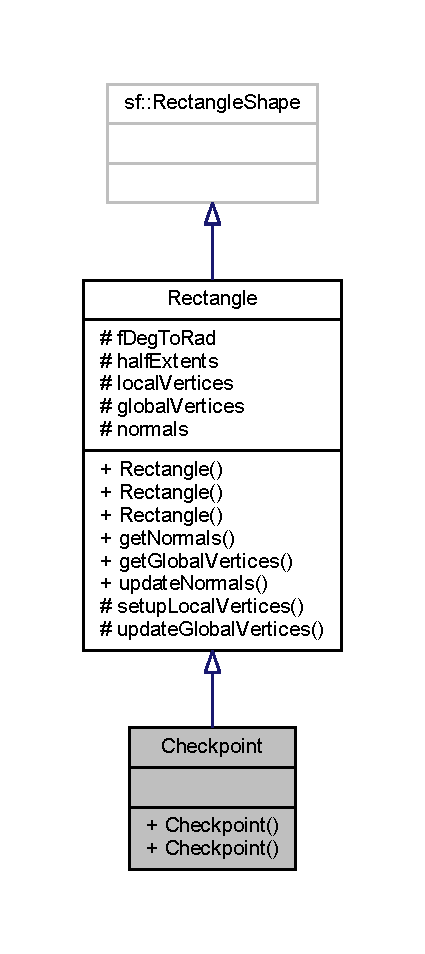
\includegraphics[width=204pt]{class_checkpoint__inherit__graph}
\end{center}
\end{figure}


Collaboration diagram for Checkpoint\+:\nopagebreak
\begin{figure}[H]
\begin{center}
\leavevmode
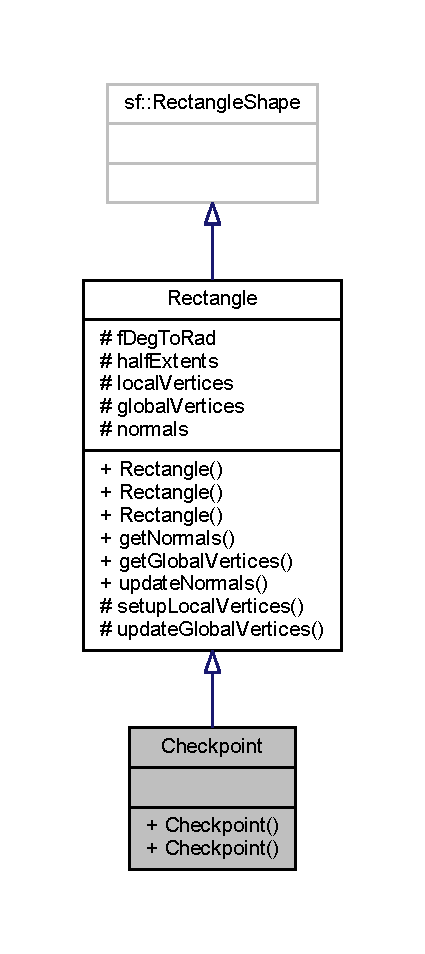
\includegraphics[width=204pt]{class_checkpoint__coll__graph}
\end{center}
\end{figure}
\subsection*{Public Member Functions}
\begin{DoxyCompactItemize}
\item 
\hyperlink{class_checkpoint_a7583dda24f192e944ebbfaad7efe4d5b}{Checkpoint} ()
\item 
\hyperlink{class_checkpoint_a27cd3de8d0680d688ed539d54bcefaf3}{Checkpoint} (const sf\+::\+Vector2f \&position, const sf\+::\+Vector2f \&dimensions, const sf\+::\+Texture \&texture, const float f\+Angle)
\end{DoxyCompactItemize}
\subsection*{Additional Inherited Members}


\subsection{Detailed Description}
This class is used to do create a simple checkpoint. 

\subsection{Constructor \& Destructor Documentation}
\index{Checkpoint@{Checkpoint}!Checkpoint@{Checkpoint}}
\index{Checkpoint@{Checkpoint}!Checkpoint@{Checkpoint}}
\subsubsection[{\texorpdfstring{Checkpoint()}{Checkpoint()}}]{\setlength{\rightskip}{0pt plus 5cm}Checkpoint\+::\+Checkpoint (
\begin{DoxyParamCaption}
{}
\end{DoxyParamCaption}
)\hspace{0.3cm}{\ttfamily [inline]}}\hypertarget{class_checkpoint_a7583dda24f192e944ebbfaad7efe4d5b}{}\label{class_checkpoint_a7583dda24f192e944ebbfaad7efe4d5b}
Initializer. \index{Checkpoint@{Checkpoint}!Checkpoint@{Checkpoint}}
\index{Checkpoint@{Checkpoint}!Checkpoint@{Checkpoint}}
\subsubsection[{\texorpdfstring{Checkpoint(const sf\+::\+Vector2f \&position, const sf\+::\+Vector2f \&dimensions, const sf\+::\+Texture \&texture, const float f\+Angle)}{Checkpoint(const sf::Vector2f &position, const sf::Vector2f &dimensions, const sf::Texture &texture, const float fAngle)}}]{\setlength{\rightskip}{0pt plus 5cm}Checkpoint\+::\+Checkpoint (
\begin{DoxyParamCaption}
\item[{const sf\+::\+Vector2f \&}]{position, }
\item[{const sf\+::\+Vector2f \&}]{dimensions, }
\item[{const sf\+::\+Texture \&}]{texture, }
\item[{const float}]{f\+Angle}
\end{DoxyParamCaption}
)}\hypertarget{class_checkpoint_a27cd3de8d0680d688ed539d54bcefaf3}{}\label{class_checkpoint_a27cd3de8d0680d688ed539d54bcefaf3}
Constructor. 
\begin{DoxyParams}{Parameters}
{\em position} & = Position of the rectangle. \\
\hline
{\em dimensions} & = Size of the rectangle. \\
\hline
{\em texture} & = Texture to load. \\
\hline
{\em f\+Angle} & = An orientation of the checkpoint \\
\hline
\end{DoxyParams}


The documentation for this class was generated from the following file\+:\begin{DoxyCompactItemize}
\item 
include/\hyperlink{checkpoint_8h}{checkpoint.\+h}\end{DoxyCompactItemize}

\hypertarget{class_circle}{}\section{Circle Class Reference}
\label{class_circle}\index{Circle@{Circle}}


This class is used to create an abstract base class of the circle.  




{\ttfamily \#include $<$circle.\+h$>$}



Inheritance diagram for Circle\+:\nopagebreak
\begin{figure}[H]
\begin{center}
\leavevmode
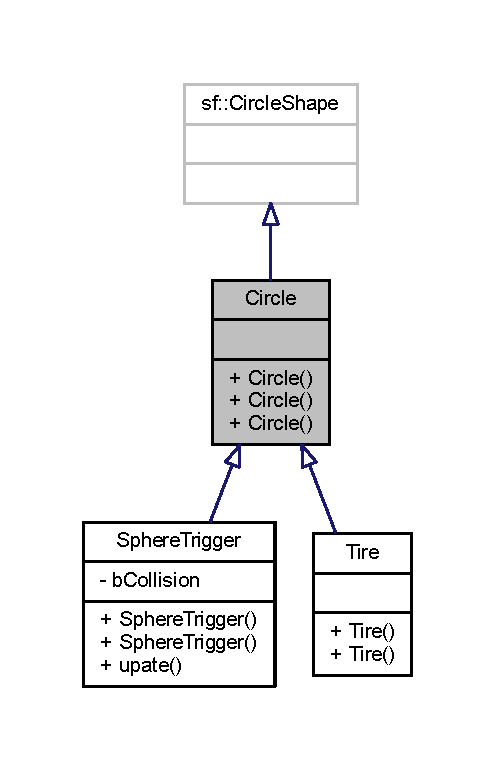
\includegraphics[width=238pt]{class_circle__inherit__graph}
\end{center}
\end{figure}


Collaboration diagram for Circle\+:\nopagebreak
\begin{figure}[H]
\begin{center}
\leavevmode
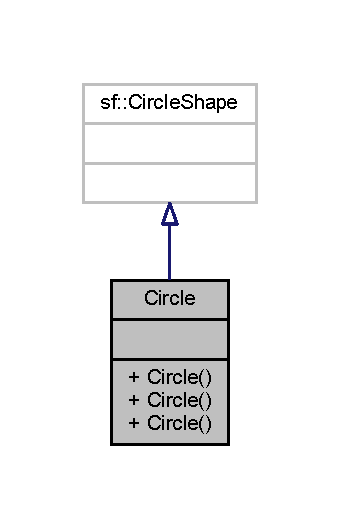
\includegraphics[width=163pt]{class_circle__coll__graph}
\end{center}
\end{figure}
\subsection*{Public Member Functions}
\begin{DoxyCompactItemize}
\item 
\hyperlink{class_circle_ad1ecfcfc7bf34529c6a6d6c448bf70fe}{Circle} ()
\item 
\hyperlink{class_circle_a0b4b28fcea9bbf75e4f44f4b6cdcc4e5}{Circle} (const sf\+::\+Vector2f \&position, float f\+Radius)
\item 
\hyperlink{class_circle_a696bed1bfe570eb852579620bd9390d7}{Circle} (sf\+::\+Vector2f \&position, float f\+Radius, sf\+::\+Texture \&texture)
\end{DoxyCompactItemize}


\subsection{Detailed Description}
This class is used to create an abstract base class of the circle. 

\subsection{Constructor \& Destructor Documentation}
\index{Circle@{Circle}!Circle@{Circle}}
\index{Circle@{Circle}!Circle@{Circle}}
\subsubsection[{\texorpdfstring{Circle()}{Circle()}}]{\setlength{\rightskip}{0pt plus 5cm}Circle\+::\+Circle (
\begin{DoxyParamCaption}
{}
\end{DoxyParamCaption}
)\hspace{0.3cm}{\ttfamily [inline]}}\hypertarget{class_circle_ad1ecfcfc7bf34529c6a6d6c448bf70fe}{}\label{class_circle_ad1ecfcfc7bf34529c6a6d6c448bf70fe}
Initializer. \index{Circle@{Circle}!Circle@{Circle}}
\index{Circle@{Circle}!Circle@{Circle}}
\subsubsection[{\texorpdfstring{Circle(const sf\+::\+Vector2f \&position, float f\+Radius)}{Circle(const sf::Vector2f &position, float fRadius)}}]{\setlength{\rightskip}{0pt plus 5cm}Circle\+::\+Circle (
\begin{DoxyParamCaption}
\item[{const sf\+::\+Vector2f \&}]{position, }
\item[{float}]{f\+Radius}
\end{DoxyParamCaption}
)}\hypertarget{class_circle_a0b4b28fcea9bbf75e4f44f4b6cdcc4e5}{}\label{class_circle_a0b4b28fcea9bbf75e4f44f4b6cdcc4e5}
Constructor. 
\begin{DoxyParams}{Parameters}
{\em position} & = Position of the circle. \\
\hline
{\em f\+Radius} & = Radius of the circle. \\
\hline
\end{DoxyParams}
\index{Circle@{Circle}!Circle@{Circle}}
\index{Circle@{Circle}!Circle@{Circle}}
\subsubsection[{\texorpdfstring{Circle(sf\+::\+Vector2f \&position, float f\+Radius, sf\+::\+Texture \&texture)}{Circle(sf::Vector2f &position, float fRadius, sf::Texture &texture)}}]{\setlength{\rightskip}{0pt plus 5cm}Circle\+::\+Circle (
\begin{DoxyParamCaption}
\item[{sf\+::\+Vector2f \&}]{position, }
\item[{float}]{f\+Radius, }
\item[{sf\+::\+Texture \&}]{texture}
\end{DoxyParamCaption}
)}\hypertarget{class_circle_a696bed1bfe570eb852579620bd9390d7}{}\label{class_circle_a696bed1bfe570eb852579620bd9390d7}
Constructor. 
\begin{DoxyParams}{Parameters}
{\em position} & = Position of the circle. \\
\hline
{\em f\+Radius} & = Radius of the circle. \\
\hline
{\em texture} & = Texture to load. \\
\hline
\end{DoxyParams}


The documentation for this class was generated from the following file\+:\begin{DoxyCompactItemize}
\item 
include/\hyperlink{circle_8h}{circle.\+h}\end{DoxyCompactItemize}

\hypertarget{class_collision}{}\section{Collision Class Reference}
\label{class_collision}\index{Collision@{Collision}}


This class is used to do collision tests.  




{\ttfamily \#include $<$collision.\+h$>$}



Collaboration diagram for Collision\+:\nopagebreak
\begin{figure}[H]
\begin{center}
\leavevmode
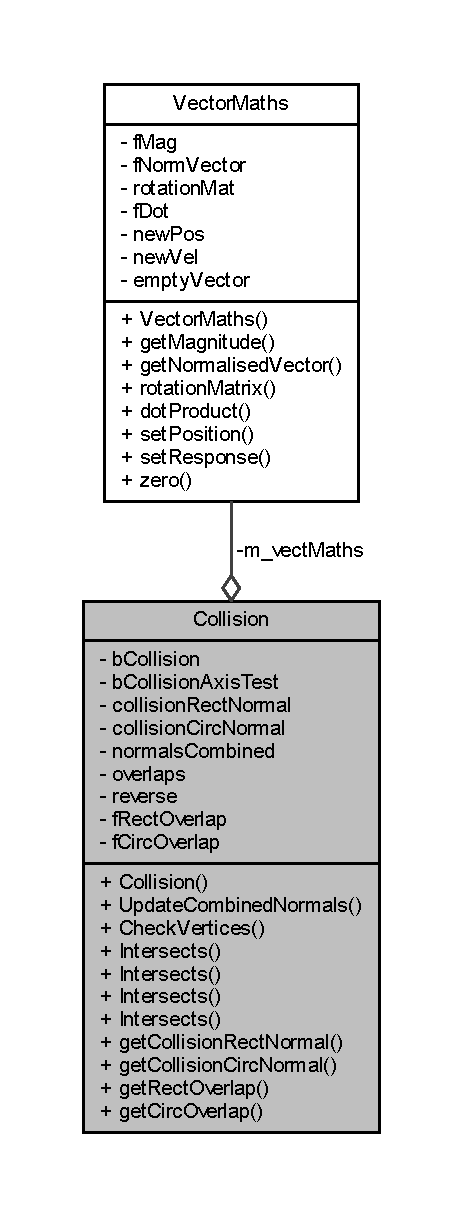
\includegraphics[height=550pt]{class_collision__coll__graph}
\end{center}
\end{figure}
\subsection*{Public Member Functions}
\begin{DoxyCompactItemize}
\item 
\hyperlink{class_collision_aea8004fbf48b79b5db7b784688b23788}{Collision} ()
\item 
void \hyperlink{class_collision_a447fe84c543fc402f1779d0771773878}{Update\+Combined\+Normals} (std\+::vector$<$ sf\+::\+Vector2f $>$ \&first, std\+::vector$<$ sf\+::\+Vector2f $>$ \&other)
\item 
void \hyperlink{class_collision_acfff38c9712d0671e466daae126eade0}{Check\+Vertices} (sf\+::\+Vertex \&vertex, sf\+::\+Vector2f \&normal, float \&f\+Min, float \&f\+Max)
\item 
bool \hyperlink{class_collision_aa449054d324451f054a312479334f006}{Intersects} (\hyperlink{class_rectangle}{Rectangle} \&first\+A\+A\+BB, \hyperlink{class_rectangle}{Rectangle} \&other\+A\+A\+BB, std\+::string s\+A\+A\+BB)
\item 
bool \hyperlink{class_collision_afe374ad46bd824d5311a805771d74d4c}{Intersects} (\hyperlink{class_rectangle}{Rectangle} \&first, \hyperlink{class_rectangle}{Rectangle} \&other)
\item 
bool \hyperlink{class_collision_a437a8d88145b86b460cd60b432cc3e9e}{Intersects} (\hyperlink{class_rectangle}{Rectangle} \&first, \hyperlink{class_circle}{Circle} \&other)
\item 
bool \hyperlink{class_collision_a6bec285cd3ceab74dbbc8c861454a973}{Intersects} (\hyperlink{class_circle}{Circle} \&first, \hyperlink{class_circle}{Circle} \&other)
\item 
sf\+::\+Vector2f \hyperlink{class_collision_af6b664b6ea60154584aa0715d7d2633a}{get\+Collision\+Rect\+Normal} ()
\item 
sf\+::\+Vector2f \hyperlink{class_collision_a1b186d29f5e80d453219098b317511d3}{get\+Collision\+Circ\+Normal} ()
\item 
float \hyperlink{class_collision_a87622ae46722faf9929bcd1b9d1183bd}{get\+Rect\+Overlap} ()
\item 
float \hyperlink{class_collision_a955a13843b8a621ec84e4201af14d418}{get\+Circ\+Overlap} ()
\end{DoxyCompactItemize}
\subsection*{Private Attributes}
\begin{DoxyCompactItemize}
\item 
bool \hyperlink{class_collision_a80db9ae6bac2cd1f032d8b2c4d7a75c5}{b\+Collision}
\item 
bool \hyperlink{class_collision_aa4a00832adce88fe922980cbaf0362a9}{b\+Collision\+Axis\+Test} \mbox{[}4\mbox{]}
\item 
sf\+::\+Vector2f \hyperlink{class_collision_a1ccb2e8e575ead01b332a65338bc92fd}{collision\+Rect\+Normal}
\item 
sf\+::\+Vector2f \hyperlink{class_collision_aed4ea8e9cafeec9b67713c2948854ee4}{collision\+Circ\+Normal}
\item 
std\+::vector$<$ sf\+::\+Vector2f $>$ \hyperlink{class_collision_aa3e126df67a5d939cfc0ec2ebac14cf5}{normals\+Combined}
\item 
std\+::vector$<$ float $>$ \hyperlink{class_collision_a789d44569f105338d670feabc02bc2ce}{overlaps}
\item 
std\+::vector$<$ float $>$ \hyperlink{class_collision_ad92247b56bd8dc65526bf9e740baa9d0}{reverse}
\item 
float \hyperlink{class_collision_a232bdb17411322d39be3dba8df18fe19}{f\+Rect\+Overlap}
\item 
float \hyperlink{class_collision_a35cb18deca301a426db25a00eb2fd504}{f\+Circ\+Overlap}
\item 
\hyperlink{class_vector_maths}{Vector\+Maths} \hyperlink{class_collision_affb289a519ea7c61695ab74e11a82b5d}{m\+\_\+vect\+Maths}
\end{DoxyCompactItemize}


\subsection{Detailed Description}
This class is used to do collision tests. 

\subsection{Constructor \& Destructor Documentation}
\index{Collision@{Collision}!Collision@{Collision}}
\index{Collision@{Collision}!Collision@{Collision}}
\subsubsection[{\texorpdfstring{Collision()}{Collision()}}]{\setlength{\rightskip}{0pt plus 5cm}Collision\+::\+Collision (
\begin{DoxyParamCaption}
{}
\end{DoxyParamCaption}
)}\hypertarget{class_collision_aea8004fbf48b79b5db7b784688b23788}{}\label{class_collision_aea8004fbf48b79b5db7b784688b23788}
An initializer. 

\subsection{Member Function Documentation}
\index{Collision@{Collision}!Check\+Vertices@{Check\+Vertices}}
\index{Check\+Vertices@{Check\+Vertices}!Collision@{Collision}}
\subsubsection[{\texorpdfstring{Check\+Vertices(sf\+::\+Vertex \&vertex, sf\+::\+Vector2f \&normal, float \&f\+Min, float \&f\+Max)}{CheckVertices(sf::Vertex &vertex, sf::Vector2f &normal, float &fMin, float &fMax)}}]{\setlength{\rightskip}{0pt plus 5cm}void Collision\+::\+Check\+Vertices (
\begin{DoxyParamCaption}
\item[{sf\+::\+Vertex \&}]{vertex, }
\item[{sf\+::\+Vector2f \&}]{normal, }
\item[{float \&}]{f\+Min, }
\item[{float \&}]{f\+Max}
\end{DoxyParamCaption}
)}\hypertarget{class_collision_acfff38c9712d0671e466daae126eade0}{}\label{class_collision_acfff38c9712d0671e466daae126eade0}
Projection of O\+BB rectangle onto axis. 
\begin{DoxyParams}{Parameters}
{\em vertex} & = A vertex of the O\+BB rectangle. \\
\hline
{\em normal} & = A face normal of the O\+BB rectangle. \\
\hline
{\em f\+Min} & = A current minimum of the O\+BB rectangle. \\
\hline
{\em f\+Max} & = A current maximum of the O\+BB rectangle. \\
\hline
\end{DoxyParams}
\index{Collision@{Collision}!get\+Circ\+Overlap@{get\+Circ\+Overlap}}
\index{get\+Circ\+Overlap@{get\+Circ\+Overlap}!Collision@{Collision}}
\subsubsection[{\texorpdfstring{get\+Circ\+Overlap()}{getCircOverlap()}}]{\setlength{\rightskip}{0pt plus 5cm}float Collision\+::get\+Circ\+Overlap (
\begin{DoxyParamCaption}
{}
\end{DoxyParamCaption}
)}\hypertarget{class_collision_a955a13843b8a621ec84e4201af14d418}{}\label{class_collision_a955a13843b8a621ec84e4201af14d418}
Returns overlap of the circle. \begin{DoxyReturn}{Returns}
std\+::abs(f\+Circ\+Overlap) = Returns a positive circle overlap. 
\end{DoxyReturn}
\index{Collision@{Collision}!get\+Collision\+Circ\+Normal@{get\+Collision\+Circ\+Normal}}
\index{get\+Collision\+Circ\+Normal@{get\+Collision\+Circ\+Normal}!Collision@{Collision}}
\subsubsection[{\texorpdfstring{get\+Collision\+Circ\+Normal()}{getCollisionCircNormal()}}]{\setlength{\rightskip}{0pt plus 5cm}sf\+::\+Vector2f Collision\+::get\+Collision\+Circ\+Normal (
\begin{DoxyParamCaption}
{}
\end{DoxyParamCaption}
)}\hypertarget{class_collision_a1b186d29f5e80d453219098b317511d3}{}\label{class_collision_a1b186d29f5e80d453219098b317511d3}
Returns collision normal of the circle. \begin{DoxyReturn}{Returns}
collision\+Circ\+Normal = \hyperlink{class_circle}{Circle} collision normal. 
\end{DoxyReturn}
\index{Collision@{Collision}!get\+Collision\+Rect\+Normal@{get\+Collision\+Rect\+Normal}}
\index{get\+Collision\+Rect\+Normal@{get\+Collision\+Rect\+Normal}!Collision@{Collision}}
\subsubsection[{\texorpdfstring{get\+Collision\+Rect\+Normal()}{getCollisionRectNormal()}}]{\setlength{\rightskip}{0pt plus 5cm}sf\+::\+Vector2f Collision\+::get\+Collision\+Rect\+Normal (
\begin{DoxyParamCaption}
{}
\end{DoxyParamCaption}
)}\hypertarget{class_collision_af6b664b6ea60154584aa0715d7d2633a}{}\label{class_collision_af6b664b6ea60154584aa0715d7d2633a}
Returns collision normal of the rectangle. \begin{DoxyReturn}{Returns}
collision\+Rect\+Normal = \hyperlink{class_rectangle}{Rectangle} collision normal. 
\end{DoxyReturn}
\index{Collision@{Collision}!get\+Rect\+Overlap@{get\+Rect\+Overlap}}
\index{get\+Rect\+Overlap@{get\+Rect\+Overlap}!Collision@{Collision}}
\subsubsection[{\texorpdfstring{get\+Rect\+Overlap()}{getRectOverlap()}}]{\setlength{\rightskip}{0pt plus 5cm}float Collision\+::get\+Rect\+Overlap (
\begin{DoxyParamCaption}
{}
\end{DoxyParamCaption}
)}\hypertarget{class_collision_a87622ae46722faf9929bcd1b9d1183bd}{}\label{class_collision_a87622ae46722faf9929bcd1b9d1183bd}
Returns overlap of the rectangle. \begin{DoxyReturn}{Returns}
f\+Rect\+Overlap = Returns a rectangle overlap. 
\end{DoxyReturn}
\index{Collision@{Collision}!Intersects@{Intersects}}
\index{Intersects@{Intersects}!Collision@{Collision}}
\subsubsection[{\texorpdfstring{Intersects(\+Rectangle \&first\+A\+A\+B\+B, Rectangle \&other\+A\+A\+B\+B, std\+::string s\+A\+A\+B\+B)}{Intersects(Rectangle &firstAABB, Rectangle &otherAABB, std::string sAABB)}}]{\setlength{\rightskip}{0pt plus 5cm}bool Collision\+::\+Intersects (
\begin{DoxyParamCaption}
\item[{{\bf Rectangle} \&}]{first\+A\+A\+BB, }
\item[{{\bf Rectangle} \&}]{other\+A\+A\+BB, }
\item[{std\+::string}]{s\+A\+A\+BB}
\end{DoxyParamCaption}
)}\hypertarget{class_collision_aa449054d324451f054a312479334f006}{}\label{class_collision_aa449054d324451f054a312479334f006}
\hyperlink{class_collision}{Collision} test A\+A\+B\+B-\/\+A\+A\+BB. 
\begin{DoxyParams}{Parameters}
{\em first\+A\+A\+BB} & = First A\+A\+BB rectangle. \\
\hline
{\em other\+A\+A\+BB} & = Second A\+A\+BB rectangle. \\
\hline
{\em s\+A\+A\+BB} & = A variable with any name to avoid overloading the O\+BB checks. \\
\hline
\end{DoxyParams}
\index{Collision@{Collision}!Intersects@{Intersects}}
\index{Intersects@{Intersects}!Collision@{Collision}}
\subsubsection[{\texorpdfstring{Intersects(\+Rectangle \&first, Rectangle \&other)}{Intersects(Rectangle &first, Rectangle &other)}}]{\setlength{\rightskip}{0pt plus 5cm}bool Collision\+::\+Intersects (
\begin{DoxyParamCaption}
\item[{{\bf Rectangle} \&}]{first, }
\item[{{\bf Rectangle} \&}]{other}
\end{DoxyParamCaption}
)}\hypertarget{class_collision_afe374ad46bd824d5311a805771d74d4c}{}\label{class_collision_afe374ad46bd824d5311a805771d74d4c}
\hyperlink{class_collision}{Collision} test O\+B\+B-\/\+O\+BB. 
\begin{DoxyParams}{Parameters}
{\em first} & = First O\+BB rectangle. \\
\hline
{\em other} & = Second O\+BB rectangle. \\
\hline
\end{DoxyParams}
\index{Collision@{Collision}!Intersects@{Intersects}}
\index{Intersects@{Intersects}!Collision@{Collision}}
\subsubsection[{\texorpdfstring{Intersects(\+Rectangle \&first, Circle \&other)}{Intersects(Rectangle &first, Circle &other)}}]{\setlength{\rightskip}{0pt plus 5cm}bool Collision\+::\+Intersects (
\begin{DoxyParamCaption}
\item[{{\bf Rectangle} \&}]{first, }
\item[{{\bf Circle} \&}]{other}
\end{DoxyParamCaption}
)}\hypertarget{class_collision_a437a8d88145b86b460cd60b432cc3e9e}{}\label{class_collision_a437a8d88145b86b460cd60b432cc3e9e}
\hyperlink{class_collision}{Collision} test O\+B\+B-\/\+Circle. 
\begin{DoxyParams}{Parameters}
{\em first} & = An O\+BB rectangle. \\
\hline
{\em other} & = A circle. \\
\hline
\end{DoxyParams}
\index{Collision@{Collision}!Intersects@{Intersects}}
\index{Intersects@{Intersects}!Collision@{Collision}}
\subsubsection[{\texorpdfstring{Intersects(\+Circle \&first, Circle \&other)}{Intersects(Circle &first, Circle &other)}}]{\setlength{\rightskip}{0pt plus 5cm}bool Collision\+::\+Intersects (
\begin{DoxyParamCaption}
\item[{{\bf Circle} \&}]{first, }
\item[{{\bf Circle} \&}]{other}
\end{DoxyParamCaption}
)}\hypertarget{class_collision_a6bec285cd3ceab74dbbc8c861454a973}{}\label{class_collision_a6bec285cd3ceab74dbbc8c861454a973}
\hyperlink{class_collision}{Collision} test O\+B\+B-\/\+Circle. 
\begin{DoxyParams}{Parameters}
{\em first} & = A first circle. \\
\hline
{\em other} & = A second circle. \\
\hline
\end{DoxyParams}
\index{Collision@{Collision}!Update\+Combined\+Normals@{Update\+Combined\+Normals}}
\index{Update\+Combined\+Normals@{Update\+Combined\+Normals}!Collision@{Collision}}
\subsubsection[{\texorpdfstring{Update\+Combined\+Normals(std\+::vector$<$ sf\+::\+Vector2f $>$ \&first, std\+::vector$<$ sf\+::\+Vector2f $>$ \&other)}{UpdateCombinedNormals(std::vector< sf::Vector2f > &first, std::vector< sf::Vector2f > &other)}}]{\setlength{\rightskip}{0pt plus 5cm}void Collision\+::\+Update\+Combined\+Normals (
\begin{DoxyParamCaption}
\item[{std\+::vector$<$ sf\+::\+Vector2f $>$ \&}]{first, }
\item[{std\+::vector$<$ sf\+::\+Vector2f $>$ \&}]{other}
\end{DoxyParamCaption}
)}\hypertarget{class_collision_a447fe84c543fc402f1779d0771773878}{}\label{class_collision_a447fe84c543fc402f1779d0771773878}
Updates normals of combined O\+BB rectangles. 
\begin{DoxyParams}{Parameters}
{\em first} & = Face normals of the first O\+BB rectangle. \\
\hline
{\em other} & = Face normals of the second O\+BB rectangle. \\
\hline
\end{DoxyParams}


\subsection{Member Data Documentation}
\index{Collision@{Collision}!b\+Collision@{b\+Collision}}
\index{b\+Collision@{b\+Collision}!Collision@{Collision}}
\subsubsection[{\texorpdfstring{b\+Collision}{bCollision}}]{\setlength{\rightskip}{0pt plus 5cm}bool Collision\+::b\+Collision\hspace{0.3cm}{\ttfamily [private]}}\hypertarget{class_collision_a80db9ae6bac2cd1f032d8b2c4d7a75c5}{}\label{class_collision_a80db9ae6bac2cd1f032d8b2c4d7a75c5}
Confrim collision. \index{Collision@{Collision}!b\+Collision\+Axis\+Test@{b\+Collision\+Axis\+Test}}
\index{b\+Collision\+Axis\+Test@{b\+Collision\+Axis\+Test}!Collision@{Collision}}
\subsubsection[{\texorpdfstring{b\+Collision\+Axis\+Test}{bCollisionAxisTest}}]{\setlength{\rightskip}{0pt plus 5cm}bool Collision\+::b\+Collision\+Axis\+Test\mbox{[}4\mbox{]}\hspace{0.3cm}{\ttfamily [private]}}\hypertarget{class_collision_aa4a00832adce88fe922980cbaf0362a9}{}\label{class_collision_aa4a00832adce88fe922980cbaf0362a9}
Confrim collision tests on axes. \index{Collision@{Collision}!collision\+Circ\+Normal@{collision\+Circ\+Normal}}
\index{collision\+Circ\+Normal@{collision\+Circ\+Normal}!Collision@{Collision}}
\subsubsection[{\texorpdfstring{collision\+Circ\+Normal}{collisionCircNormal}}]{\setlength{\rightskip}{0pt plus 5cm}sf\+::\+Vector2f Collision\+::collision\+Circ\+Normal\hspace{0.3cm}{\ttfamily [private]}}\hypertarget{class_collision_aed4ea8e9cafeec9b67713c2948854ee4}{}\label{class_collision_aed4ea8e9cafeec9b67713c2948854ee4}
\hyperlink{class_circle}{Circle} collision normal. \index{Collision@{Collision}!collision\+Rect\+Normal@{collision\+Rect\+Normal}}
\index{collision\+Rect\+Normal@{collision\+Rect\+Normal}!Collision@{Collision}}
\subsubsection[{\texorpdfstring{collision\+Rect\+Normal}{collisionRectNormal}}]{\setlength{\rightskip}{0pt plus 5cm}sf\+::\+Vector2f Collision\+::collision\+Rect\+Normal\hspace{0.3cm}{\ttfamily [private]}}\hypertarget{class_collision_a1ccb2e8e575ead01b332a65338bc92fd}{}\label{class_collision_a1ccb2e8e575ead01b332a65338bc92fd}
\hyperlink{class_rectangle}{Rectangle} collision normal. \index{Collision@{Collision}!f\+Circ\+Overlap@{f\+Circ\+Overlap}}
\index{f\+Circ\+Overlap@{f\+Circ\+Overlap}!Collision@{Collision}}
\subsubsection[{\texorpdfstring{f\+Circ\+Overlap}{fCircOverlap}}]{\setlength{\rightskip}{0pt plus 5cm}float Collision\+::f\+Circ\+Overlap\hspace{0.3cm}{\ttfamily [private]}}\hypertarget{class_collision_a35cb18deca301a426db25a00eb2fd504}{}\label{class_collision_a35cb18deca301a426db25a00eb2fd504}
\hyperlink{class_circle}{Circle} overlap. \index{Collision@{Collision}!f\+Rect\+Overlap@{f\+Rect\+Overlap}}
\index{f\+Rect\+Overlap@{f\+Rect\+Overlap}!Collision@{Collision}}
\subsubsection[{\texorpdfstring{f\+Rect\+Overlap}{fRectOverlap}}]{\setlength{\rightskip}{0pt plus 5cm}float Collision\+::f\+Rect\+Overlap\hspace{0.3cm}{\ttfamily [private]}}\hypertarget{class_collision_a232bdb17411322d39be3dba8df18fe19}{}\label{class_collision_a232bdb17411322d39be3dba8df18fe19}
\hyperlink{class_rectangle}{Rectangle} overlap. \index{Collision@{Collision}!m\+\_\+vect\+Maths@{m\+\_\+vect\+Maths}}
\index{m\+\_\+vect\+Maths@{m\+\_\+vect\+Maths}!Collision@{Collision}}
\subsubsection[{\texorpdfstring{m\+\_\+vect\+Maths}{m_vectMaths}}]{\setlength{\rightskip}{0pt plus 5cm}{\bf Vector\+Maths} Collision\+::m\+\_\+vect\+Maths\hspace{0.3cm}{\ttfamily [private]}}\hypertarget{class_collision_affb289a519ea7c61695ab74e11a82b5d}{}\label{class_collision_affb289a519ea7c61695ab74e11a82b5d}
A variable which deals with vector maths. \index{Collision@{Collision}!normals\+Combined@{normals\+Combined}}
\index{normals\+Combined@{normals\+Combined}!Collision@{Collision}}
\subsubsection[{\texorpdfstring{normals\+Combined}{normalsCombined}}]{\setlength{\rightskip}{0pt plus 5cm}std\+::vector$<$sf\+::\+Vector2f$>$ Collision\+::normals\+Combined\hspace{0.3cm}{\ttfamily [private]}}\hypertarget{class_collision_aa3e126df67a5d939cfc0ec2ebac14cf5}{}\label{class_collision_aa3e126df67a5d939cfc0ec2ebac14cf5}
Combined rectangle face normals. \index{Collision@{Collision}!overlaps@{overlaps}}
\index{overlaps@{overlaps}!Collision@{Collision}}
\subsubsection[{\texorpdfstring{overlaps}{overlaps}}]{\setlength{\rightskip}{0pt plus 5cm}std\+::vector$<$float$>$ Collision\+::overlaps\hspace{0.3cm}{\ttfamily [private]}}\hypertarget{class_collision_a789d44569f105338d670feabc02bc2ce}{}\label{class_collision_a789d44569f105338d670feabc02bc2ce}
Vector with overlaps from O\+BB tests. \index{Collision@{Collision}!reverse@{reverse}}
\index{reverse@{reverse}!Collision@{Collision}}
\subsubsection[{\texorpdfstring{reverse}{reverse}}]{\setlength{\rightskip}{0pt plus 5cm}std\+::vector$<$float$>$ Collision\+::reverse\hspace{0.3cm}{\ttfamily [private]}}\hypertarget{class_collision_ad92247b56bd8dc65526bf9e740baa9d0}{}\label{class_collision_ad92247b56bd8dc65526bf9e740baa9d0}
Vector with reverses from O\+BB tests. 

The documentation for this class was generated from the following file\+:\begin{DoxyCompactItemize}
\item 
include/\hyperlink{collision_8h}{collision.\+h}\end{DoxyCompactItemize}

\hypertarget{class_font_loader}{}\section{Font\+Loader Class Reference}
\label{class_font_loader}\index{Font\+Loader@{Font\+Loader}}


This class is used to manage fonts.  




{\ttfamily \#include $<$font\+Loader.\+h$>$}



Collaboration diagram for Font\+Loader\+:\nopagebreak
\begin{figure}[H]
\begin{center}
\leavevmode
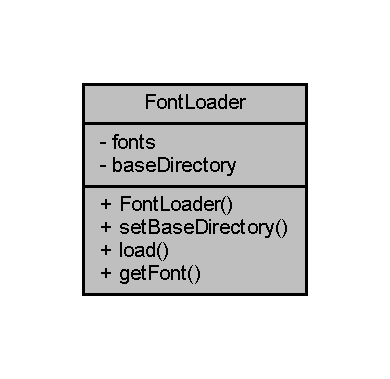
\includegraphics[width=187pt]{class_font_loader__coll__graph}
\end{center}
\end{figure}
\subsection*{Public Member Functions}
\begin{DoxyCompactItemize}
\item 
\hyperlink{class_font_loader_a425b3451baedece1c0cbfa884dd0972a}{Font\+Loader} ()
\item 
void \hyperlink{class_font_loader_a47fd7f5d01ae1c5c687962c3d696f7e0}{set\+Base\+Directory} (std\+::string dir)
\item 
void \hyperlink{class_font_loader_ad78b54b629f95a5940779caa9914e8f7}{load} (std\+::vector$<$ std\+::string $>$ file\+Names)
\item 
sf\+::\+Font \& \hyperlink{class_font_loader_a9927072242d4d8c5b800a471527c9d93}{get\+Font} (int f\+Index)
\end{DoxyCompactItemize}
\subsection*{Private Attributes}
\begin{DoxyCompactItemize}
\item 
std\+::vector$<$ sf\+::\+Font $>$ \hyperlink{class_font_loader_abe3d75dec9d31a88cbfc889df83d2916}{fonts}
\item 
std\+::string \hyperlink{class_font_loader_af5430afdc542c29683315bb331e75efc}{base\+Directory}
\end{DoxyCompactItemize}


\subsection{Detailed Description}
This class is used to manage fonts. 

\subsection{Constructor \& Destructor Documentation}
\index{Font\+Loader@{Font\+Loader}!Font\+Loader@{Font\+Loader}}
\index{Font\+Loader@{Font\+Loader}!Font\+Loader@{Font\+Loader}}
\subsubsection[{\texorpdfstring{Font\+Loader()}{FontLoader()}}]{\setlength{\rightskip}{0pt plus 5cm}Font\+Loader\+::\+Font\+Loader (
\begin{DoxyParamCaption}
{}
\end{DoxyParamCaption}
)}\hypertarget{class_font_loader_a425b3451baedece1c0cbfa884dd0972a}{}\label{class_font_loader_a425b3451baedece1c0cbfa884dd0972a}
An initializer. 

\subsection{Member Function Documentation}
\index{Font\+Loader@{Font\+Loader}!get\+Font@{get\+Font}}
\index{get\+Font@{get\+Font}!Font\+Loader@{Font\+Loader}}
\subsubsection[{\texorpdfstring{get\+Font(int f\+Index)}{getFont(int fIndex)}}]{\setlength{\rightskip}{0pt plus 5cm}sf\+::\+Font\& Font\+Loader\+::get\+Font (
\begin{DoxyParamCaption}
\item[{int}]{f\+Index}
\end{DoxyParamCaption}
)}\hypertarget{class_font_loader_a9927072242d4d8c5b800a471527c9d93}{}\label{class_font_loader_a9927072242d4d8c5b800a471527c9d93}
Returns a font with said index. 
\begin{DoxyParams}{Parameters}
{\em f\+Index} & = Index of the font. \\
\hline
\end{DoxyParams}
\begin{DoxyReturn}{Returns}
$\ast$it = Retruns pointer to the font with matching index. 
\end{DoxyReturn}
\index{Font\+Loader@{Font\+Loader}!load@{load}}
\index{load@{load}!Font\+Loader@{Font\+Loader}}
\subsubsection[{\texorpdfstring{load(std\+::vector$<$ std\+::string $>$ file\+Names)}{load(std::vector< std::string > fileNames)}}]{\setlength{\rightskip}{0pt plus 5cm}void Font\+Loader\+::load (
\begin{DoxyParamCaption}
\item[{std\+::vector$<$ std\+::string $>$}]{file\+Names}
\end{DoxyParamCaption}
)}\hypertarget{class_font_loader_ad78b54b629f95a5940779caa9914e8f7}{}\label{class_font_loader_ad78b54b629f95a5940779caa9914e8f7}
Loads fonts based on the string input. 
\begin{DoxyParams}{Parameters}
{\em file\+Names} & = String vector with file names. \\
\hline
\end{DoxyParams}
\index{Font\+Loader@{Font\+Loader}!set\+Base\+Directory@{set\+Base\+Directory}}
\index{set\+Base\+Directory@{set\+Base\+Directory}!Font\+Loader@{Font\+Loader}}
\subsubsection[{\texorpdfstring{set\+Base\+Directory(std\+::string dir)}{setBaseDirectory(std::string dir)}}]{\setlength{\rightskip}{0pt plus 5cm}void Font\+Loader\+::set\+Base\+Directory (
\begin{DoxyParamCaption}
\item[{std\+::string}]{dir}
\end{DoxyParamCaption}
)}\hypertarget{class_font_loader_a47fd7f5d01ae1c5c687962c3d696f7e0}{}\label{class_font_loader_a47fd7f5d01ae1c5c687962c3d696f7e0}
Sets our base directory. 
\begin{DoxyParams}{Parameters}
{\em dir} & = Our base directory. \\
\hline
\end{DoxyParams}


\subsection{Member Data Documentation}
\index{Font\+Loader@{Font\+Loader}!base\+Directory@{base\+Directory}}
\index{base\+Directory@{base\+Directory}!Font\+Loader@{Font\+Loader}}
\subsubsection[{\texorpdfstring{base\+Directory}{baseDirectory}}]{\setlength{\rightskip}{0pt plus 5cm}std\+::string Font\+Loader\+::base\+Directory\hspace{0.3cm}{\ttfamily [private]}}\hypertarget{class_font_loader_af5430afdc542c29683315bb331e75efc}{}\label{class_font_loader_af5430afdc542c29683315bb331e75efc}
Our base directory with fonts. \index{Font\+Loader@{Font\+Loader}!fonts@{fonts}}
\index{fonts@{fonts}!Font\+Loader@{Font\+Loader}}
\subsubsection[{\texorpdfstring{fonts}{fonts}}]{\setlength{\rightskip}{0pt plus 5cm}std\+::vector$<$sf\+::\+Font$>$ Font\+Loader\+::fonts\hspace{0.3cm}{\ttfamily [private]}}\hypertarget{class_font_loader_abe3d75dec9d31a88cbfc889df83d2916}{}\label{class_font_loader_abe3d75dec9d31a88cbfc889df83d2916}
Vector of fonts. 

The documentation for this class was generated from the following file\+:\begin{DoxyCompactItemize}
\item 
include/\hyperlink{font_loader_8h}{font\+Loader.\+h}\end{DoxyCompactItemize}

\hypertarget{class_game}{}\section{Game Class Reference}
\label{class_game}\index{Game@{Game}}


This class is used to create a game window.  




{\ttfamily \#include $<$game.\+h$>$}



Inheritance diagram for Game\+:\nopagebreak
\begin{figure}[H]
\begin{center}
\leavevmode
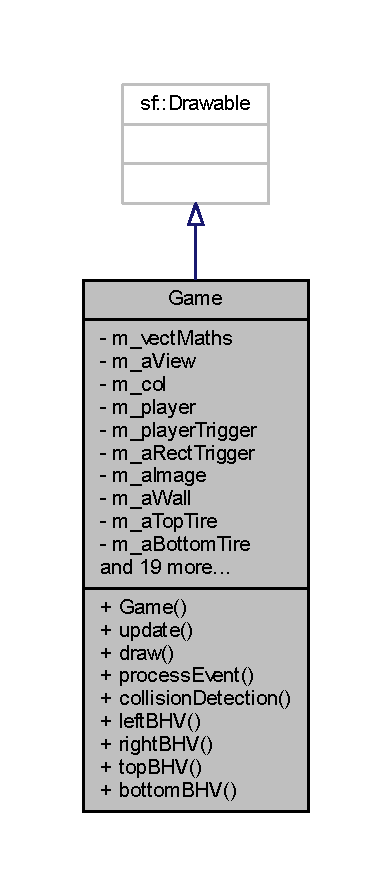
\includegraphics[width=188pt]{class_game__inherit__graph}
\end{center}
\end{figure}


Collaboration diagram for Game\+:\nopagebreak
\begin{figure}[H]
\begin{center}
\leavevmode
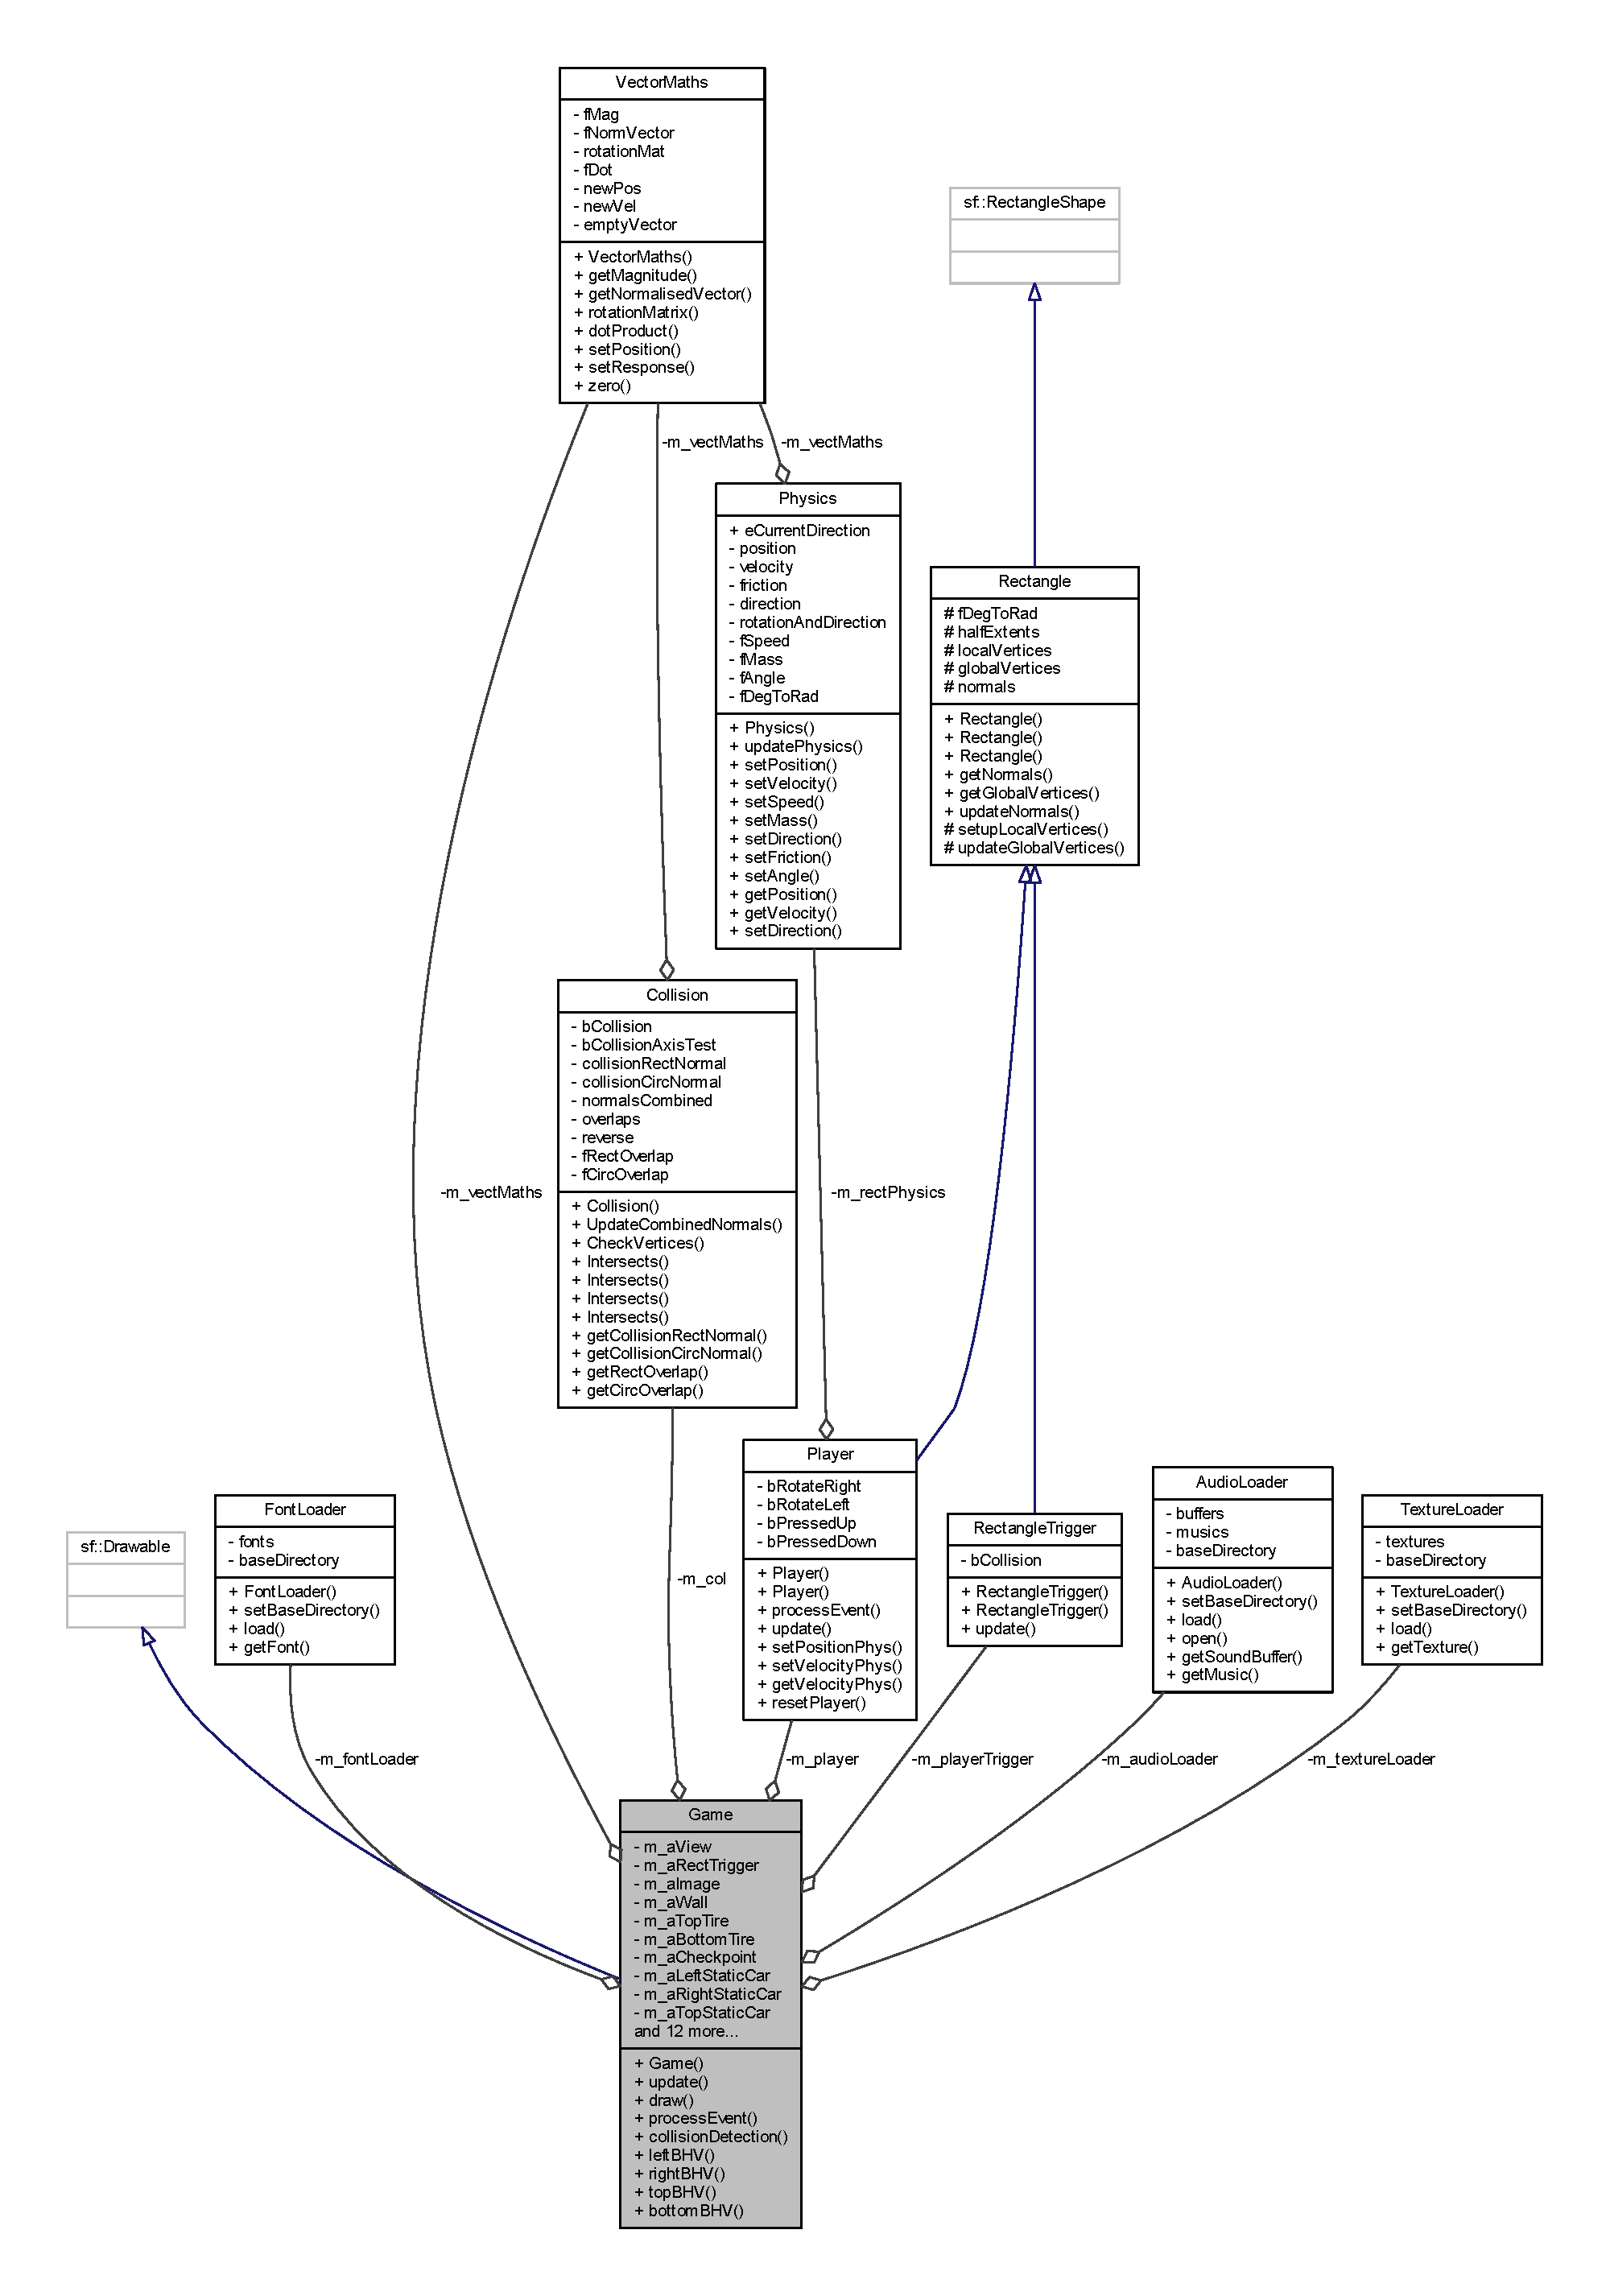
\includegraphics[width=350pt]{class_game__coll__graph}
\end{center}
\end{figure}
\subsection*{Public Member Functions}
\begin{DoxyCompactItemize}
\item 
\hyperlink{class_game_ad59df6562a58a614fda24622d3715b65}{Game} ()
\item 
void \hyperlink{class_game_a92a5eb842e5b304e89dc2caf530f7a6d}{update} (float time\+Step)
\item 
void \hyperlink{class_game_a43337462c32106b3374a86a12a242ba0}{draw} (sf\+::\+Render\+Target \&target, sf\+::\+Render\+States states) const 
\item 
void \hyperlink{class_game_a53c3821c70ba6acb541bdbefac8d037c}{process\+Event} (sf\+::\+Event \&e, sf\+::\+Render\+Window \&window)
\item 
void \hyperlink{class_game_a04598b31d30614a0eda08dd8b3dcecb9}{collision\+Detection} ()
\item 
void \hyperlink{class_game_aea043c436651fa28343224e1e51c9e24}{left\+B\+HV} ()
\item 
void \hyperlink{class_game_a69f84b7c0e4565c690b22eb195937a00}{right\+B\+HV} ()
\item 
void \hyperlink{class_game_aa6b8153a760fbf3cef5e30157be3ee45}{top\+B\+HV} ()
\item 
void \hyperlink{class_game_ab974c9d1736297e36b8b91e3faaee637}{bottom\+B\+HV} ()
\end{DoxyCompactItemize}
\subsection*{Private Types}
\begin{DoxyCompactItemize}
\item 
enum \hyperlink{class_game_a7f57a7a8408e554d0a72882c287e1d04}{Game\+State} \{ \hyperlink{class_game_a7f57a7a8408e554d0a72882c287e1d04afa4424e746d7d1082d6e27c4811f3984}{Start}, 
\hyperlink{class_game_a7f57a7a8408e554d0a72882c287e1d04afc89c8495fe7b84c06560b6aa6195bbf}{Reset}, 
\hyperlink{class_game_a7f57a7a8408e554d0a72882c287e1d04ac5a0d20c5cb7b20c0f6cca50edeed64f}{Playing}, 
\hyperlink{class_game_a7f57a7a8408e554d0a72882c287e1d04ab2cf7098808338abae856bf46ac82b91}{Pause}
 \}
\end{DoxyCompactItemize}
\subsection*{Private Attributes}
\begin{DoxyCompactItemize}
\item 
\hyperlink{class_vector_maths}{Vector\+Maths} \hyperlink{class_game_a2f535f85fe3b454b9c708993753f4ecc}{m\+\_\+vect\+Maths}
\item 
std\+::array$<$ \hyperlink{class_view}{View}, 3 $>$ \hyperlink{class_game_a36d2bed14974b11445cb7a4da0256adf}{m\+\_\+a\+View}
\item 
\hyperlink{class_collision}{Collision} \hyperlink{class_game_ac35fe5a8537b15105621229bdfa0e282}{m\+\_\+col}
\item 
\hyperlink{class_player}{Player} \hyperlink{class_game_ad1f796902ca353bad4c877939e0005e7}{m\+\_\+player}
\item 
\hyperlink{class_rectangle_trigger}{Rectangle\+Trigger} \hyperlink{class_game_a007f25af28324cc117c00239be5c167b}{m\+\_\+player\+Trigger}
\item 
std\+::array$<$ \hyperlink{class_rectangle_trigger}{Rectangle\+Trigger}, 11 $>$ \hyperlink{class_game_a2065f8dee8f173a73ef904525ab6823e}{m\+\_\+a\+Rect\+Trigger}
\item 
std\+::array$<$ \hyperlink{class_image}{Image}, 3 $>$ \hyperlink{class_game_a5025f591142de524119d0dcc99300d3b}{m\+\_\+a\+Image}
\item 
std\+::array$<$ \hyperlink{class_wall}{Wall}, 2 $>$ \hyperlink{class_game_a3baabf1657a540fb01d7c256829f4221}{m\+\_\+a\+Wall}
\item 
std\+::array$<$ \hyperlink{class_tire}{Tire}, 17 $>$ \hyperlink{class_game_a3b92928693ffa8c38f8e11c032990def}{m\+\_\+a\+Top\+Tire}
\item 
std\+::array$<$ \hyperlink{class_tire}{Tire}, 17 $>$ \hyperlink{class_game_a15992ccedd036df35c2e8c14b70676ef}{m\+\_\+a\+Bottom\+Tire}
\item 
std\+::array$<$ \hyperlink{class_checkpoint}{Checkpoint}, 4 $>$ \hyperlink{class_game_ade427c88bcff6dd2e4b7e78a6db93f04}{m\+\_\+a\+Checkpoint}
\item 
std\+::array$<$ \hyperlink{class_static_car}{Static\+Car}, 3 $>$ \hyperlink{class_game_a664151ff15f6aaecc56b1c35e7fb05df}{m\+\_\+a\+Left\+Static\+Car}
\item 
std\+::array$<$ \hyperlink{class_static_car}{Static\+Car}, 3 $>$ \hyperlink{class_game_a53199784b896c76c8b6fc7663f92b334}{m\+\_\+a\+Right\+Static\+Car}
\item 
std\+::array$<$ \hyperlink{class_static_car}{Static\+Car}, 2 $>$ \hyperlink{class_game_ac8205b8f1930f12fd4fdd71ab575bbdf}{m\+\_\+a\+Top\+Static\+Car}
\item 
std\+::array$<$ \hyperlink{class_static_car}{Static\+Car}, 2 $>$ \hyperlink{class_game_a0af48a2f04c50bfcb3d961dbd1a48332}{m\+\_\+a\+Bottom\+Static\+Car}
\item 
std\+::array$<$ sf\+::\+Sound, 1 $>$ \hyperlink{class_game_a9bbec66f60fb732629222dd90ba62778}{m\+\_\+a\+Sound}
\item 
std\+::vector$<$ std\+::string $>$ \hyperlink{class_game_afd0a84adb730239bae2eed9a8eded08e}{s\+File\+Name\+Texture}
\item 
std\+::vector$<$ std\+::string $>$ \hyperlink{class_game_a4989e4e035912a6cd8d00c8b2e627b43}{s\+File\+Name\+Font}
\item 
std\+::vector$<$ std\+::string $>$ \hyperlink{class_game_ad6b42e850d075a49c003f32fba1a2dd1}{s\+File\+Name\+Music}
\item 
std\+::vector$<$ std\+::string $>$ \hyperlink{class_game_a4bff69d4d76477050669e7f10d8d1da8}{s\+File\+Name\+Sound}
\item 
\hyperlink{class_texture_loader}{Texture\+Loader} \hyperlink{class_game_a361590f1fa6617f110b614b232b00631}{m\+\_\+texture\+Loader}
\item 
\hyperlink{class_font_loader}{Font\+Loader} \hyperlink{class_game_aa9d87d7d97d1651a68cc0301861e86e3}{m\+\_\+font\+Loader}
\item 
\hyperlink{class_audio_loader}{Audio\+Loader} \hyperlink{class_game_a4012ccf746dc592aff5ede39df9e2b17}{m\+\_\+audio\+Loader}
\item 
std\+::array$<$ \hyperlink{class_simple_text}{Simple\+Text}, 4 $>$ \hyperlink{class_game_a8a9e4f882c541075d13cad25ea2aec08}{m\+\_\+a\+Text}
\item 
sf\+::\+Clock \hyperlink{class_game_afa2b2cd71f1808971458e67a8540a83d}{m\+\_\+clock}
\item 
int \hyperlink{class_game_a377116aa9d1b98c95fc42f593bfefc33}{i\+Time}
\item 
int \hyperlink{class_game_a67d656a5608c3cd5cd3df69932bb16fb}{i\+Lap}
\item 
bool \hyperlink{class_game_a7eda5a4db623fc9e05fad674c9b9e6bb}{b\+Lap\+Confirm} \mbox{[}4\mbox{]}
\item 
\hyperlink{class_game_a7f57a7a8408e554d0a72882c287e1d04}{Game\+State} \hyperlink{class_game_ae0322dfc4abedec88046d09ca3460f35}{e\+Current\+State}
\end{DoxyCompactItemize}


\subsection{Detailed Description}
This class is used to create a game window. 

\subsection{Member Enumeration Documentation}
\index{Game@{Game}!Game\+State@{Game\+State}}
\index{Game\+State@{Game\+State}!Game@{Game}}
\subsubsection[{\texorpdfstring{Game\+State}{GameState}}]{\setlength{\rightskip}{0pt plus 5cm}enum {\bf Game\+::\+Game\+State}\hspace{0.3cm}{\ttfamily [private]}}\hypertarget{class_game_a7f57a7a8408e554d0a72882c287e1d04}{}\label{class_game_a7f57a7a8408e554d0a72882c287e1d04}
\hyperlink{class_game}{Game} states. \begin{Desc}
\item[Enumerator]\par
\begin{description}
\index{Start@{Start}!Game@{Game}}\index{Game@{Game}!Start@{Start}}\item[{\em 
Start\hypertarget{class_game_a7f57a7a8408e554d0a72882c287e1d04afa4424e746d7d1082d6e27c4811f3984}{}\label{class_game_a7f57a7a8408e554d0a72882c287e1d04afa4424e746d7d1082d6e27c4811f3984}
}]Start = We are starting the game. \index{Reset@{Reset}!Game@{Game}}\index{Game@{Game}!Reset@{Reset}}\item[{\em 
Reset\hypertarget{class_game_a7f57a7a8408e554d0a72882c287e1d04afc89c8495fe7b84c06560b6aa6195bbf}{}\label{class_game_a7f57a7a8408e554d0a72882c287e1d04afc89c8495fe7b84c06560b6aa6195bbf}
}]Reset = We are resetting game variables. \index{Playing@{Playing}!Game@{Game}}\index{Game@{Game}!Playing@{Playing}}\item[{\em 
Playing\hypertarget{class_game_a7f57a7a8408e554d0a72882c287e1d04ac5a0d20c5cb7b20c0f6cca50edeed64f}{}\label{class_game_a7f57a7a8408e554d0a72882c287e1d04ac5a0d20c5cb7b20c0f6cca50edeed64f}
}]Playing = We are playing the game. \index{Pause@{Pause}!Game@{Game}}\index{Game@{Game}!Pause@{Pause}}\item[{\em 
Pause\hypertarget{class_game_a7f57a7a8408e554d0a72882c287e1d04ab2cf7098808338abae856bf46ac82b91}{}\label{class_game_a7f57a7a8408e554d0a72882c287e1d04ab2cf7098808338abae856bf46ac82b91}
}]Pause = \hyperlink{class_player}{Player} has finished the game. \end{description}
\end{Desc}


\subsection{Constructor \& Destructor Documentation}
\index{Game@{Game}!Game@{Game}}
\index{Game@{Game}!Game@{Game}}
\subsubsection[{\texorpdfstring{Game()}{Game()}}]{\setlength{\rightskip}{0pt plus 5cm}Game\+::\+Game (
\begin{DoxyParamCaption}
{}
\end{DoxyParamCaption}
)}\hypertarget{class_game_ad59df6562a58a614fda24622d3715b65}{}\label{class_game_ad59df6562a58a614fda24622d3715b65}
An initializer. 

\subsection{Member Function Documentation}
\index{Game@{Game}!bottom\+B\+HV@{bottom\+B\+HV}}
\index{bottom\+B\+HV@{bottom\+B\+HV}!Game@{Game}}
\subsubsection[{\texorpdfstring{bottom\+B\+H\+V()}{bottomBHV()}}]{\setlength{\rightskip}{0pt plus 5cm}void Game\+::bottom\+B\+HV (
\begin{DoxyParamCaption}
{}
\end{DoxyParamCaption}
)}\hypertarget{class_game_ab974c9d1736297e36b8b91e3faaee637}{}\label{class_game_ab974c9d1736297e36b8b91e3faaee637}
Bounding Volume Hierarchies -\/ Bottom. \index{Game@{Game}!collision\+Detection@{collision\+Detection}}
\index{collision\+Detection@{collision\+Detection}!Game@{Game}}
\subsubsection[{\texorpdfstring{collision\+Detection()}{collisionDetection()}}]{\setlength{\rightskip}{0pt plus 5cm}void Game\+::collision\+Detection (
\begin{DoxyParamCaption}
{}
\end{DoxyParamCaption}
)}\hypertarget{class_game_a04598b31d30614a0eda08dd8b3dcecb9}{}\label{class_game_a04598b31d30614a0eda08dd8b3dcecb9}
All collision detection is done in here. \index{Game@{Game}!draw@{draw}}
\index{draw@{draw}!Game@{Game}}
\subsubsection[{\texorpdfstring{draw(sf\+::\+Render\+Target \&target, sf\+::\+Render\+States states) const }{draw(sf::RenderTarget &target, sf::RenderStates states) const }}]{\setlength{\rightskip}{0pt plus 5cm}void Game\+::draw (
\begin{DoxyParamCaption}
\item[{sf\+::\+Render\+Target \&}]{target, }
\item[{sf\+::\+Render\+States}]{states}
\end{DoxyParamCaption}
) const}\hypertarget{class_game_a43337462c32106b3374a86a12a242ba0}{}\label{class_game_a43337462c32106b3374a86a12a242ba0}
Drawing objects. 
\begin{DoxyParams}{Parameters}
{\em target} & = Render target to draw to. \\
\hline
{\em states} & = Current render states. \\
\hline
\end{DoxyParams}
\index{Game@{Game}!left\+B\+HV@{left\+B\+HV}}
\index{left\+B\+HV@{left\+B\+HV}!Game@{Game}}
\subsubsection[{\texorpdfstring{left\+B\+H\+V()}{leftBHV()}}]{\setlength{\rightskip}{0pt plus 5cm}void Game\+::left\+B\+HV (
\begin{DoxyParamCaption}
{}
\end{DoxyParamCaption}
)}\hypertarget{class_game_aea043c436651fa28343224e1e51c9e24}{}\label{class_game_aea043c436651fa28343224e1e51c9e24}
Bounding Volume Hierarchies -\/ Left side. \index{Game@{Game}!process\+Event@{process\+Event}}
\index{process\+Event@{process\+Event}!Game@{Game}}
\subsubsection[{\texorpdfstring{process\+Event(sf\+::\+Event \&e, sf\+::\+Render\+Window \&window)}{processEvent(sf::Event &e, sf::RenderWindow &window)}}]{\setlength{\rightskip}{0pt plus 5cm}void Game\+::process\+Event (
\begin{DoxyParamCaption}
\item[{sf\+::\+Event \&}]{e, }
\item[{sf\+::\+Render\+Window \&}]{window}
\end{DoxyParamCaption}
)}\hypertarget{class_game_a53c3821c70ba6acb541bdbefac8d037c}{}\label{class_game_a53c3821c70ba6acb541bdbefac8d037c}
Process any key events. 
\begin{DoxyParams}{Parameters}
{\em e} & = Event variable needed to capture any key presses. \\
\hline
{\em window} & = Takes a window variable so that we can process events to it \\
\hline
\end{DoxyParams}
\index{Game@{Game}!right\+B\+HV@{right\+B\+HV}}
\index{right\+B\+HV@{right\+B\+HV}!Game@{Game}}
\subsubsection[{\texorpdfstring{right\+B\+H\+V()}{rightBHV()}}]{\setlength{\rightskip}{0pt plus 5cm}void Game\+::right\+B\+HV (
\begin{DoxyParamCaption}
{}
\end{DoxyParamCaption}
)}\hypertarget{class_game_a69f84b7c0e4565c690b22eb195937a00}{}\label{class_game_a69f84b7c0e4565c690b22eb195937a00}
Bounding Volume Hierarchies -\/ Right side. \index{Game@{Game}!top\+B\+HV@{top\+B\+HV}}
\index{top\+B\+HV@{top\+B\+HV}!Game@{Game}}
\subsubsection[{\texorpdfstring{top\+B\+H\+V()}{topBHV()}}]{\setlength{\rightskip}{0pt plus 5cm}void Game\+::top\+B\+HV (
\begin{DoxyParamCaption}
{}
\end{DoxyParamCaption}
)}\hypertarget{class_game_aa6b8153a760fbf3cef5e30157be3ee45}{}\label{class_game_aa6b8153a760fbf3cef5e30157be3ee45}
Bounding Volume Hierarchies -\/ Top. \index{Game@{Game}!update@{update}}
\index{update@{update}!Game@{Game}}
\subsubsection[{\texorpdfstring{update(float time\+Step)}{update(float timeStep)}}]{\setlength{\rightskip}{0pt plus 5cm}void Game\+::update (
\begin{DoxyParamCaption}
\item[{float}]{time\+Step}
\end{DoxyParamCaption}
)}\hypertarget{class_game_a92a5eb842e5b304e89dc2caf530f7a6d}{}\label{class_game_a92a5eb842e5b304e89dc2caf530f7a6d}
\hyperlink{class_game}{Game} update. 
\begin{DoxyParams}{Parameters}
{\em time\+Step} & = Time which updates most of the functions and variables, for example velocity. \\
\hline
\end{DoxyParams}


\subsection{Member Data Documentation}
\index{Game@{Game}!b\+Lap\+Confirm@{b\+Lap\+Confirm}}
\index{b\+Lap\+Confirm@{b\+Lap\+Confirm}!Game@{Game}}
\subsubsection[{\texorpdfstring{b\+Lap\+Confirm}{bLapConfirm}}]{\setlength{\rightskip}{0pt plus 5cm}bool Game\+::b\+Lap\+Confirm\mbox{[}4\mbox{]}\hspace{0.3cm}{\ttfamily [private]}}\hypertarget{class_game_a7eda5a4db623fc9e05fad674c9b9e6bb}{}\label{class_game_a7eda5a4db623fc9e05fad674c9b9e6bb}
Lap confirmation. \index{Game@{Game}!e\+Current\+State@{e\+Current\+State}}
\index{e\+Current\+State@{e\+Current\+State}!Game@{Game}}
\subsubsection[{\texorpdfstring{e\+Current\+State}{eCurrentState}}]{\setlength{\rightskip}{0pt plus 5cm}{\bf Game\+State} Game\+::e\+Current\+State\hspace{0.3cm}{\ttfamily [private]}}\hypertarget{class_game_ae0322dfc4abedec88046d09ca3460f35}{}\label{class_game_ae0322dfc4abedec88046d09ca3460f35}
\index{Game@{Game}!i\+Lap@{i\+Lap}}
\index{i\+Lap@{i\+Lap}!Game@{Game}}
\subsubsection[{\texorpdfstring{i\+Lap}{iLap}}]{\setlength{\rightskip}{0pt plus 5cm}int Game\+::i\+Lap\hspace{0.3cm}{\ttfamily [private]}}\hypertarget{class_game_a67d656a5608c3cd5cd3df69932bb16fb}{}\label{class_game_a67d656a5608c3cd5cd3df69932bb16fb}
Lap counter. \index{Game@{Game}!i\+Time@{i\+Time}}
\index{i\+Time@{i\+Time}!Game@{Game}}
\subsubsection[{\texorpdfstring{i\+Time}{iTime}}]{\setlength{\rightskip}{0pt plus 5cm}int Game\+::i\+Time\hspace{0.3cm}{\ttfamily [private]}}\hypertarget{class_game_a377116aa9d1b98c95fc42f593bfefc33}{}\label{class_game_a377116aa9d1b98c95fc42f593bfefc33}
Time tracker. \index{Game@{Game}!m\+\_\+a\+Bottom\+Static\+Car@{m\+\_\+a\+Bottom\+Static\+Car}}
\index{m\+\_\+a\+Bottom\+Static\+Car@{m\+\_\+a\+Bottom\+Static\+Car}!Game@{Game}}
\subsubsection[{\texorpdfstring{m\+\_\+a\+Bottom\+Static\+Car}{m_aBottomStaticCar}}]{\setlength{\rightskip}{0pt plus 5cm}std\+::array$<${\bf Static\+Car}, 2$>$ Game\+::m\+\_\+a\+Bottom\+Static\+Car\hspace{0.3cm}{\ttfamily [private]}}\hypertarget{class_game_a0af48a2f04c50bfcb3d961dbd1a48332}{}\label{class_game_a0af48a2f04c50bfcb3d961dbd1a48332}
An array of cars positioned on the top. \index{Game@{Game}!m\+\_\+a\+Bottom\+Tire@{m\+\_\+a\+Bottom\+Tire}}
\index{m\+\_\+a\+Bottom\+Tire@{m\+\_\+a\+Bottom\+Tire}!Game@{Game}}
\subsubsection[{\texorpdfstring{m\+\_\+a\+Bottom\+Tire}{m_aBottomTire}}]{\setlength{\rightskip}{0pt plus 5cm}std\+::array$<${\bf Tire}, 17$>$ Game\+::m\+\_\+a\+Bottom\+Tire\hspace{0.3cm}{\ttfamily [private]}}\hypertarget{class_game_a15992ccedd036df35c2e8c14b70676ef}{}\label{class_game_a15992ccedd036df35c2e8c14b70676ef}
An array of tires positioned at the bottom of the screen. \index{Game@{Game}!m\+\_\+a\+Checkpoint@{m\+\_\+a\+Checkpoint}}
\index{m\+\_\+a\+Checkpoint@{m\+\_\+a\+Checkpoint}!Game@{Game}}
\subsubsection[{\texorpdfstring{m\+\_\+a\+Checkpoint}{m_aCheckpoint}}]{\setlength{\rightskip}{0pt plus 5cm}std\+::array$<${\bf Checkpoint}, 4$>$ Game\+::m\+\_\+a\+Checkpoint\hspace{0.3cm}{\ttfamily [private]}}\hypertarget{class_game_ade427c88bcff6dd2e4b7e78a6db93f04}{}\label{class_game_ade427c88bcff6dd2e4b7e78a6db93f04}
An array of checkpoints positioned in the world. \index{Game@{Game}!m\+\_\+a\+Image@{m\+\_\+a\+Image}}
\index{m\+\_\+a\+Image@{m\+\_\+a\+Image}!Game@{Game}}
\subsubsection[{\texorpdfstring{m\+\_\+a\+Image}{m_aImage}}]{\setlength{\rightskip}{0pt plus 5cm}std\+::array$<${\bf Image}, 3$>$ Game\+::m\+\_\+a\+Image\hspace{0.3cm}{\ttfamily [private]}}\hypertarget{class_game_a5025f591142de524119d0dcc99300d3b}{}\label{class_game_a5025f591142de524119d0dcc99300d3b}
An array of images \index{Game@{Game}!m\+\_\+a\+Left\+Static\+Car@{m\+\_\+a\+Left\+Static\+Car}}
\index{m\+\_\+a\+Left\+Static\+Car@{m\+\_\+a\+Left\+Static\+Car}!Game@{Game}}
\subsubsection[{\texorpdfstring{m\+\_\+a\+Left\+Static\+Car}{m_aLeftStaticCar}}]{\setlength{\rightskip}{0pt plus 5cm}std\+::array$<${\bf Static\+Car}, 3$>$ Game\+::m\+\_\+a\+Left\+Static\+Car\hspace{0.3cm}{\ttfamily [private]}}\hypertarget{class_game_a664151ff15f6aaecc56b1c35e7fb05df}{}\label{class_game_a664151ff15f6aaecc56b1c35e7fb05df}
An array of cars positioned on the left. \index{Game@{Game}!m\+\_\+a\+Rect\+Trigger@{m\+\_\+a\+Rect\+Trigger}}
\index{m\+\_\+a\+Rect\+Trigger@{m\+\_\+a\+Rect\+Trigger}!Game@{Game}}
\subsubsection[{\texorpdfstring{m\+\_\+a\+Rect\+Trigger}{m_aRectTrigger}}]{\setlength{\rightskip}{0pt plus 5cm}std\+::array$<${\bf Rectangle\+Trigger}, 11$>$ Game\+::m\+\_\+a\+Rect\+Trigger\hspace{0.3cm}{\ttfamily [private]}}\hypertarget{class_game_a2065f8dee8f173a73ef904525ab6823e}{}\label{class_game_a2065f8dee8f173a73ef904525ab6823e}
An array of rectangle triggers for the objects \index{Game@{Game}!m\+\_\+a\+Right\+Static\+Car@{m\+\_\+a\+Right\+Static\+Car}}
\index{m\+\_\+a\+Right\+Static\+Car@{m\+\_\+a\+Right\+Static\+Car}!Game@{Game}}
\subsubsection[{\texorpdfstring{m\+\_\+a\+Right\+Static\+Car}{m_aRightStaticCar}}]{\setlength{\rightskip}{0pt plus 5cm}std\+::array$<${\bf Static\+Car}, 3$>$ Game\+::m\+\_\+a\+Right\+Static\+Car\hspace{0.3cm}{\ttfamily [private]}}\hypertarget{class_game_a53199784b896c76c8b6fc7663f92b334}{}\label{class_game_a53199784b896c76c8b6fc7663f92b334}
An array of cars positioned on the right. \index{Game@{Game}!m\+\_\+a\+Sound@{m\+\_\+a\+Sound}}
\index{m\+\_\+a\+Sound@{m\+\_\+a\+Sound}!Game@{Game}}
\subsubsection[{\texorpdfstring{m\+\_\+a\+Sound}{m_aSound}}]{\setlength{\rightskip}{0pt plus 5cm}std\+::array$<$sf\+::\+Sound, 1$>$ Game\+::m\+\_\+a\+Sound\hspace{0.3cm}{\ttfamily [private]}}\hypertarget{class_game_a9bbec66f60fb732629222dd90ba62778}{}\label{class_game_a9bbec66f60fb732629222dd90ba62778}
An array of sounds. \index{Game@{Game}!m\+\_\+a\+Text@{m\+\_\+a\+Text}}
\index{m\+\_\+a\+Text@{m\+\_\+a\+Text}!Game@{Game}}
\subsubsection[{\texorpdfstring{m\+\_\+a\+Text}{m_aText}}]{\setlength{\rightskip}{0pt plus 5cm}std\+::array$<${\bf Simple\+Text}, 4$>$ Game\+::m\+\_\+a\+Text\hspace{0.3cm}{\ttfamily [private]}}\hypertarget{class_game_a8a9e4f882c541075d13cad25ea2aec08}{}\label{class_game_a8a9e4f882c541075d13cad25ea2aec08}
An array of texts. \index{Game@{Game}!m\+\_\+a\+Top\+Static\+Car@{m\+\_\+a\+Top\+Static\+Car}}
\index{m\+\_\+a\+Top\+Static\+Car@{m\+\_\+a\+Top\+Static\+Car}!Game@{Game}}
\subsubsection[{\texorpdfstring{m\+\_\+a\+Top\+Static\+Car}{m_aTopStaticCar}}]{\setlength{\rightskip}{0pt plus 5cm}std\+::array$<${\bf Static\+Car}, 2$>$ Game\+::m\+\_\+a\+Top\+Static\+Car\hspace{0.3cm}{\ttfamily [private]}}\hypertarget{class_game_ac8205b8f1930f12fd4fdd71ab575bbdf}{}\label{class_game_ac8205b8f1930f12fd4fdd71ab575bbdf}
An array of cars positioned on the top. \index{Game@{Game}!m\+\_\+a\+Top\+Tire@{m\+\_\+a\+Top\+Tire}}
\index{m\+\_\+a\+Top\+Tire@{m\+\_\+a\+Top\+Tire}!Game@{Game}}
\subsubsection[{\texorpdfstring{m\+\_\+a\+Top\+Tire}{m_aTopTire}}]{\setlength{\rightskip}{0pt plus 5cm}std\+::array$<${\bf Tire}, 17$>$ Game\+::m\+\_\+a\+Top\+Tire\hspace{0.3cm}{\ttfamily [private]}}\hypertarget{class_game_a3b92928693ffa8c38f8e11c032990def}{}\label{class_game_a3b92928693ffa8c38f8e11c032990def}
An array of tires positioned at the top of the screen. \index{Game@{Game}!m\+\_\+audio\+Loader@{m\+\_\+audio\+Loader}}
\index{m\+\_\+audio\+Loader@{m\+\_\+audio\+Loader}!Game@{Game}}
\subsubsection[{\texorpdfstring{m\+\_\+audio\+Loader}{m_audioLoader}}]{\setlength{\rightskip}{0pt plus 5cm}{\bf Audio\+Loader} Game\+::m\+\_\+audio\+Loader\hspace{0.3cm}{\ttfamily [private]}}\hypertarget{class_game_a4012ccf746dc592aff5ede39df9e2b17}{}\label{class_game_a4012ccf746dc592aff5ede39df9e2b17}
An audio loader. \index{Game@{Game}!m\+\_\+a\+View@{m\+\_\+a\+View}}
\index{m\+\_\+a\+View@{m\+\_\+a\+View}!Game@{Game}}
\subsubsection[{\texorpdfstring{m\+\_\+a\+View}{m_aView}}]{\setlength{\rightskip}{0pt plus 5cm}std\+::array$<${\bf View}, 3$>$ Game\+::m\+\_\+a\+View\hspace{0.3cm}{\ttfamily [private]}}\hypertarget{class_game_a36d2bed14974b11445cb7a4da0256adf}{}\label{class_game_a36d2bed14974b11445cb7a4da0256adf}
An array of views. \index{Game@{Game}!m\+\_\+a\+Wall@{m\+\_\+a\+Wall}}
\index{m\+\_\+a\+Wall@{m\+\_\+a\+Wall}!Game@{Game}}
\subsubsection[{\texorpdfstring{m\+\_\+a\+Wall}{m_aWall}}]{\setlength{\rightskip}{0pt plus 5cm}std\+::array$<${\bf Wall}, 2$>$ Game\+::m\+\_\+a\+Wall\hspace{0.3cm}{\ttfamily [private]}}\hypertarget{class_game_a3baabf1657a540fb01d7c256829f4221}{}\label{class_game_a3baabf1657a540fb01d7c256829f4221}
An array of walls positioned in the world. \index{Game@{Game}!m\+\_\+clock@{m\+\_\+clock}}
\index{m\+\_\+clock@{m\+\_\+clock}!Game@{Game}}
\subsubsection[{\texorpdfstring{m\+\_\+clock}{m_clock}}]{\setlength{\rightskip}{0pt plus 5cm}sf\+::\+Clock Game\+::m\+\_\+clock\hspace{0.3cm}{\ttfamily [private]}}\hypertarget{class_game_afa2b2cd71f1808971458e67a8540a83d}{}\label{class_game_afa2b2cd71f1808971458e67a8540a83d}
Clock needed to track the time. \index{Game@{Game}!m\+\_\+col@{m\+\_\+col}}
\index{m\+\_\+col@{m\+\_\+col}!Game@{Game}}
\subsubsection[{\texorpdfstring{m\+\_\+col}{m_col}}]{\setlength{\rightskip}{0pt plus 5cm}{\bf Collision} Game\+::m\+\_\+col\hspace{0.3cm}{\ttfamily [private]}}\hypertarget{class_game_ac35fe5a8537b15105621229bdfa0e282}{}\label{class_game_ac35fe5a8537b15105621229bdfa0e282}
A collision. \index{Game@{Game}!m\+\_\+font\+Loader@{m\+\_\+font\+Loader}}
\index{m\+\_\+font\+Loader@{m\+\_\+font\+Loader}!Game@{Game}}
\subsubsection[{\texorpdfstring{m\+\_\+font\+Loader}{m_fontLoader}}]{\setlength{\rightskip}{0pt plus 5cm}{\bf Font\+Loader} Game\+::m\+\_\+font\+Loader\hspace{0.3cm}{\ttfamily [private]}}\hypertarget{class_game_aa9d87d7d97d1651a68cc0301861e86e3}{}\label{class_game_aa9d87d7d97d1651a68cc0301861e86e3}
A font loader. \index{Game@{Game}!m\+\_\+player@{m\+\_\+player}}
\index{m\+\_\+player@{m\+\_\+player}!Game@{Game}}
\subsubsection[{\texorpdfstring{m\+\_\+player}{m_player}}]{\setlength{\rightskip}{0pt plus 5cm}{\bf Player} Game\+::m\+\_\+player\hspace{0.3cm}{\ttfamily [private]}}\hypertarget{class_game_ad1f796902ca353bad4c877939e0005e7}{}\label{class_game_ad1f796902ca353bad4c877939e0005e7}
A player. \index{Game@{Game}!m\+\_\+player\+Trigger@{m\+\_\+player\+Trigger}}
\index{m\+\_\+player\+Trigger@{m\+\_\+player\+Trigger}!Game@{Game}}
\subsubsection[{\texorpdfstring{m\+\_\+player\+Trigger}{m_playerTrigger}}]{\setlength{\rightskip}{0pt plus 5cm}{\bf Rectangle\+Trigger} Game\+::m\+\_\+player\+Trigger\hspace{0.3cm}{\ttfamily [private]}}\hypertarget{class_game_a007f25af28324cc117c00239be5c167b}{}\label{class_game_a007f25af28324cc117c00239be5c167b}
Sphere trigger for the player \index{Game@{Game}!m\+\_\+texture\+Loader@{m\+\_\+texture\+Loader}}
\index{m\+\_\+texture\+Loader@{m\+\_\+texture\+Loader}!Game@{Game}}
\subsubsection[{\texorpdfstring{m\+\_\+texture\+Loader}{m_textureLoader}}]{\setlength{\rightskip}{0pt plus 5cm}{\bf Texture\+Loader} Game\+::m\+\_\+texture\+Loader\hspace{0.3cm}{\ttfamily [private]}}\hypertarget{class_game_a361590f1fa6617f110b614b232b00631}{}\label{class_game_a361590f1fa6617f110b614b232b00631}
A texture loader. \index{Game@{Game}!m\+\_\+vect\+Maths@{m\+\_\+vect\+Maths}}
\index{m\+\_\+vect\+Maths@{m\+\_\+vect\+Maths}!Game@{Game}}
\subsubsection[{\texorpdfstring{m\+\_\+vect\+Maths}{m_vectMaths}}]{\setlength{\rightskip}{0pt plus 5cm}{\bf Vector\+Maths} Game\+::m\+\_\+vect\+Maths\hspace{0.3cm}{\ttfamily [private]}}\hypertarget{class_game_a2f535f85fe3b454b9c708993753f4ecc}{}\label{class_game_a2f535f85fe3b454b9c708993753f4ecc}
A variable which deals with vector maths. \index{Game@{Game}!s\+File\+Name\+Font@{s\+File\+Name\+Font}}
\index{s\+File\+Name\+Font@{s\+File\+Name\+Font}!Game@{Game}}
\subsubsection[{\texorpdfstring{s\+File\+Name\+Font}{sFileNameFont}}]{\setlength{\rightskip}{0pt plus 5cm}std\+::vector$<$std\+::string$>$ Game\+::s\+File\+Name\+Font\hspace{0.3cm}{\ttfamily [private]}}\hypertarget{class_game_a4989e4e035912a6cd8d00c8b2e627b43}{}\label{class_game_a4989e4e035912a6cd8d00c8b2e627b43}
A vector of file names with fonts. \index{Game@{Game}!s\+File\+Name\+Music@{s\+File\+Name\+Music}}
\index{s\+File\+Name\+Music@{s\+File\+Name\+Music}!Game@{Game}}
\subsubsection[{\texorpdfstring{s\+File\+Name\+Music}{sFileNameMusic}}]{\setlength{\rightskip}{0pt plus 5cm}std\+::vector$<$std\+::string$>$ Game\+::s\+File\+Name\+Music\hspace{0.3cm}{\ttfamily [private]}}\hypertarget{class_game_ad6b42e850d075a49c003f32fba1a2dd1}{}\label{class_game_ad6b42e850d075a49c003f32fba1a2dd1}
A vector of file names with music. \index{Game@{Game}!s\+File\+Name\+Sound@{s\+File\+Name\+Sound}}
\index{s\+File\+Name\+Sound@{s\+File\+Name\+Sound}!Game@{Game}}
\subsubsection[{\texorpdfstring{s\+File\+Name\+Sound}{sFileNameSound}}]{\setlength{\rightskip}{0pt plus 5cm}std\+::vector$<$std\+::string$>$ Game\+::s\+File\+Name\+Sound\hspace{0.3cm}{\ttfamily [private]}}\hypertarget{class_game_a4bff69d4d76477050669e7f10d8d1da8}{}\label{class_game_a4bff69d4d76477050669e7f10d8d1da8}
A vector of file names with sound effects. \index{Game@{Game}!s\+File\+Name\+Texture@{s\+File\+Name\+Texture}}
\index{s\+File\+Name\+Texture@{s\+File\+Name\+Texture}!Game@{Game}}
\subsubsection[{\texorpdfstring{s\+File\+Name\+Texture}{sFileNameTexture}}]{\setlength{\rightskip}{0pt plus 5cm}std\+::vector$<$std\+::string$>$ Game\+::s\+File\+Name\+Texture\hspace{0.3cm}{\ttfamily [private]}}\hypertarget{class_game_afd0a84adb730239bae2eed9a8eded08e}{}\label{class_game_afd0a84adb730239bae2eed9a8eded08e}
A vector of file names with textures. 

The documentation for this class was generated from the following file\+:\begin{DoxyCompactItemize}
\item 
include/\hyperlink{game_8h}{game.\+h}\end{DoxyCompactItemize}

\hypertarget{class_image}{}\section{Image Class Reference}
\label{class_image}\index{Image@{Image}}


This class is used to construct an image.  




{\ttfamily \#include $<$image.\+h$>$}



Inheritance diagram for Image\+:\nopagebreak
\begin{figure}[H]
\begin{center}
\leavevmode
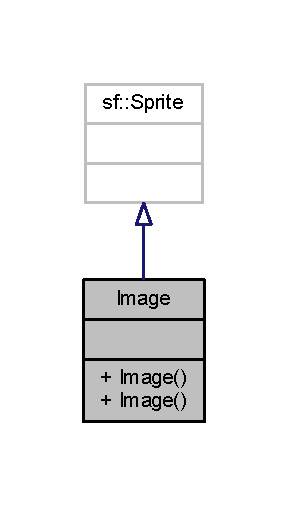
\includegraphics[width=138pt]{class_image__inherit__graph}
\end{center}
\end{figure}


Collaboration diagram for Image\+:\nopagebreak
\begin{figure}[H]
\begin{center}
\leavevmode
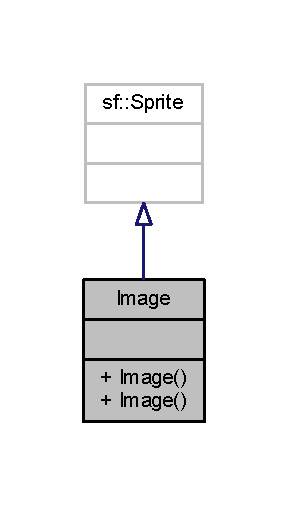
\includegraphics[width=138pt]{class_image__coll__graph}
\end{center}
\end{figure}
\subsection*{Public Member Functions}
\begin{DoxyCompactItemize}
\item 
\hyperlink{class_image_a58edd1c45b4faeb5f789b0d036d02313}{Image} ()
\item 
\hyperlink{class_image_a44769e8385de7cecfa1141900f844c70}{Image} (sf\+::\+Vector2f \&position, sf\+::\+Vector2f \&dimensions, sf\+::\+Texture \&texture)
\end{DoxyCompactItemize}


\subsection{Detailed Description}
This class is used to construct an image. 

\subsection{Constructor \& Destructor Documentation}
\index{Image@{Image}!Image@{Image}}
\index{Image@{Image}!Image@{Image}}
\subsubsection[{\texorpdfstring{Image()}{Image()}}]{\setlength{\rightskip}{0pt plus 5cm}Image\+::\+Image (
\begin{DoxyParamCaption}
{}
\end{DoxyParamCaption}
)\hspace{0.3cm}{\ttfamily [inline]}}\hypertarget{class_image_a58edd1c45b4faeb5f789b0d036d02313}{}\label{class_image_a58edd1c45b4faeb5f789b0d036d02313}
An initializer. \index{Image@{Image}!Image@{Image}}
\index{Image@{Image}!Image@{Image}}
\subsubsection[{\texorpdfstring{Image(sf\+::\+Vector2f \&position, sf\+::\+Vector2f \&dimensions, sf\+::\+Texture \&texture)}{Image(sf::Vector2f &position, sf::Vector2f &dimensions, sf::Texture &texture)}}]{\setlength{\rightskip}{0pt plus 5cm}Image\+::\+Image (
\begin{DoxyParamCaption}
\item[{sf\+::\+Vector2f \&}]{position, }
\item[{sf\+::\+Vector2f \&}]{dimensions, }
\item[{sf\+::\+Texture \&}]{texture}
\end{DoxyParamCaption}
)}\hypertarget{class_image_a44769e8385de7cecfa1141900f844c70}{}\label{class_image_a44769e8385de7cecfa1141900f844c70}
Constructor. 
\begin{DoxyParams}{Parameters}
{\em position} & = Position of the image. \\
\hline
{\em dimensions} & = Size of the image. \\
\hline
{\em texture} & = Texture to load. \\
\hline
\end{DoxyParams}


The documentation for this class was generated from the following file\+:\begin{DoxyCompactItemize}
\item 
include/\hyperlink{image_8h}{image.\+h}\end{DoxyCompactItemize}

\hypertarget{class_physics}{}\section{Physics Class Reference}
\label{class_physics}\index{Physics@{Physics}}


This class is used to create a simulation of movement.  




{\ttfamily \#include $<$physics.\+h$>$}



Collaboration diagram for Physics\+:\nopagebreak
\begin{figure}[H]
\begin{center}
\leavevmode
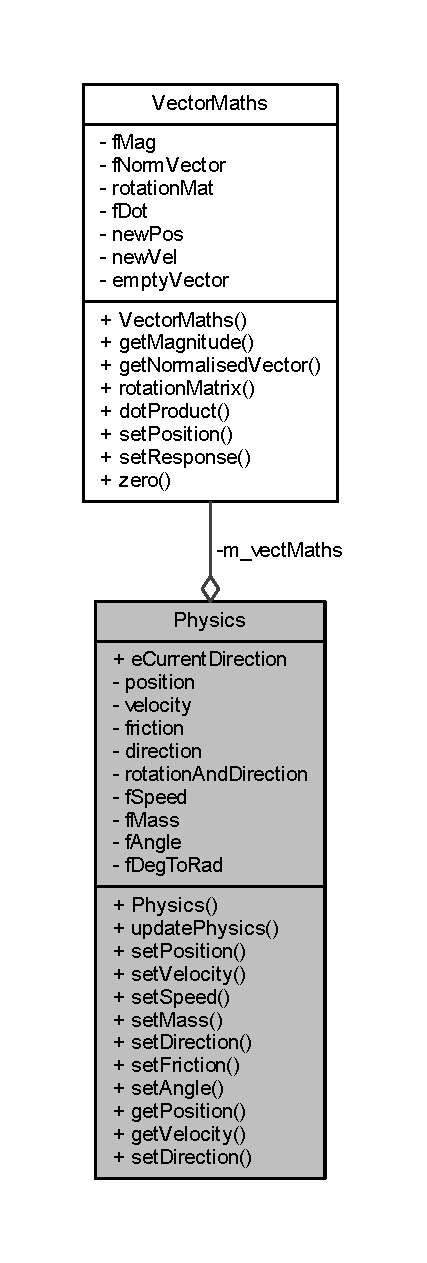
\includegraphics[height=550pt]{class_physics__coll__graph}
\end{center}
\end{figure}
\subsection*{Public Types}
\begin{DoxyCompactItemize}
\item 
enum \hyperlink{class_physics_a1a1b46dea83abe0c604a68e5445bc262}{Direction} \{ \hyperlink{class_physics_a1a1b46dea83abe0c604a68e5445bc262aee1222ec3203c2f189fb3d053b6ac4fc}{Positive}, 
\hyperlink{class_physics_a1a1b46dea83abe0c604a68e5445bc262a4563248323abfa601d3f612cea15aab9}{Negative}, 
\hyperlink{class_physics_a1a1b46dea83abe0c604a68e5445bc262afbf8fc5e7a2dab2acece07666c794ada}{None}
 \}
\end{DoxyCompactItemize}
\subsection*{Public Member Functions}
\begin{DoxyCompactItemize}
\item 
\hyperlink{class_physics_a4b2ebc0a344f04f48d227c72f0d0fbda}{Physics} ()
\item 
void \hyperlink{class_physics_a4191263a39bf65d69e90abe84801ea40}{update\+Physics} (float time\+Step)
\item 
void \hyperlink{class_physics_a74bcf0849c1fa84ac63b8b0a175cc886}{set\+Position} (sf\+::\+Vector2f \hyperlink{class_physics_a6087213b48f4754b6d69d94f0bc7606c}{position})
\item 
void \hyperlink{class_physics_ac7be95abda3d0c54bb8bb8f08854e2ae}{set\+Velocity} (sf\+::\+Vector2f new\+Vel)
\item 
void \hyperlink{class_physics_ad40c9ed00ca4051de0c94ac65405e700}{set\+Speed} (float f\+New\+Speed)
\item 
void \hyperlink{class_physics_ae5aef8654b224a3ea17cde032d8ea7b9}{set\+Mass} (float f\+New\+Mass)
\item 
void \hyperlink{class_physics_a123721942a1552796edd3c7c660779a2}{set\+Direction} (sf\+::\+Vector2f new\+Dir)
\item 
void \hyperlink{class_physics_a3869e0c4c8e23d5876f9b5b0cfdc7d2b}{set\+Friction} (sf\+::\+Vector2f new\+Fri)
\item 
void \hyperlink{class_physics_a659dfde50434b6fc3c70e51c06e1bca6}{set\+Angle} (float f\+New\+Angle)
\item 
sf\+::\+Vector2f \hyperlink{class_physics_aea92d796c2db1257df84dfed335a70fe}{get\+Position} () const 
\item 
sf\+::\+Vector2f \hyperlink{class_physics_a1f988396a60883b9a68b381f0210dfe0}{get\+Velocity} () const 
\item 
void \hyperlink{class_physics_a0122a4cac2428d85aa715ee5a6cb8170}{set\+Direction} (\hyperlink{class_physics_a1a1b46dea83abe0c604a68e5445bc262}{Direction} e\+Direction)
\end{DoxyCompactItemize}
\subsection*{Public Attributes}
\begin{DoxyCompactItemize}
\item 
\hyperlink{class_physics_a1a1b46dea83abe0c604a68e5445bc262}{Direction} \hyperlink{class_physics_ab58bbe849c871adc33364138e6777971}{e\+Current\+Direction}
\end{DoxyCompactItemize}
\subsection*{Private Attributes}
\begin{DoxyCompactItemize}
\item 
sf\+::\+Vector2f \hyperlink{class_physics_a6087213b48f4754b6d69d94f0bc7606c}{position}
\item 
sf\+::\+Vector2f \hyperlink{class_physics_ad8a150e8d89daeb6bcc0d3504b33b47d}{velocity}
\item 
sf\+::\+Vector2f \hyperlink{class_physics_ac40c58642c2fe90699cc49ac96501e2d}{friction}
\item 
sf\+::\+Vector2f \hyperlink{class_physics_a36bdbab2b563f5f5676f80780bec1207}{direction}
\item 
sf\+::\+Vector2f \hyperlink{class_physics_adc767d131b02d48ef12a87f9be293cb8}{rotation\+And\+Direction}
\item 
float \hyperlink{class_physics_a92809fe4df116f0a8c39ffd0c78ce25d}{f\+Speed}
\item 
float \hyperlink{class_physics_ac3484295b9b951d5a44105dd307f6043}{f\+Mass}
\item 
float \hyperlink{class_physics_a80e4f969bbf284b0ace8261527e4b232}{f\+Angle}
\item 
float \hyperlink{class_physics_af1307fcecb1d916f395ebcbcae254eb5}{f\+Deg\+To\+Rad}
\begin{DoxyCompactList}\small\item\em (float)M\+\_\+\+PI / 180.\+f; \end{DoxyCompactList}\item 
\hyperlink{class_vector_maths}{Vector\+Maths} \hyperlink{class_physics_a5ef3c448cb1b2c02522b3aa2c3bdc521}{m\+\_\+vect\+Maths}
\end{DoxyCompactItemize}


\subsection{Detailed Description}
This class is used to create a simulation of movement. 

\subsection{Member Enumeration Documentation}
\index{Physics@{Physics}!Direction@{Direction}}
\index{Direction@{Direction}!Physics@{Physics}}
\subsubsection[{\texorpdfstring{Direction}{Direction}}]{\setlength{\rightskip}{0pt plus 5cm}enum {\bf Physics\+::\+Direction}}\hypertarget{class_physics_a1a1b46dea83abe0c604a68e5445bc262}{}\label{class_physics_a1a1b46dea83abe0c604a68e5445bc262}
The direction that our object faces. \begin{Desc}
\item[Enumerator]\par
\begin{description}
\index{Positive@{Positive}!Physics@{Physics}}\index{Physics@{Physics}!Positive@{Positive}}\item[{\em 
Positive\hypertarget{class_physics_a1a1b46dea83abe0c604a68e5445bc262aee1222ec3203c2f189fb3d053b6ac4fc}{}\label{class_physics_a1a1b46dea83abe0c604a68e5445bc262aee1222ec3203c2f189fb3d053b6ac4fc}
}]Positive direction = We are going down. \index{Negative@{Negative}!Physics@{Physics}}\index{Physics@{Physics}!Negative@{Negative}}\item[{\em 
Negative\hypertarget{class_physics_a1a1b46dea83abe0c604a68e5445bc262a4563248323abfa601d3f612cea15aab9}{}\label{class_physics_a1a1b46dea83abe0c604a68e5445bc262a4563248323abfa601d3f612cea15aab9}
}]Negative direction = We are going up. \index{None@{None}!Physics@{Physics}}\index{Physics@{Physics}!None@{None}}\item[{\em 
None\hypertarget{class_physics_a1a1b46dea83abe0c604a68e5445bc262afbf8fc5e7a2dab2acece07666c794ada}{}\label{class_physics_a1a1b46dea83abe0c604a68e5445bc262afbf8fc5e7a2dab2acece07666c794ada}
}]None = We are not moving. \end{description}
\end{Desc}


\subsection{Constructor \& Destructor Documentation}
\index{Physics@{Physics}!Physics@{Physics}}
\index{Physics@{Physics}!Physics@{Physics}}
\subsubsection[{\texorpdfstring{Physics()}{Physics()}}]{\setlength{\rightskip}{0pt plus 5cm}Physics\+::\+Physics (
\begin{DoxyParamCaption}
{}
\end{DoxyParamCaption}
)}\hypertarget{class_physics_a4b2ebc0a344f04f48d227c72f0d0fbda}{}\label{class_physics_a4b2ebc0a344f04f48d227c72f0d0fbda}
An initializer. 

\subsection{Member Function Documentation}
\index{Physics@{Physics}!get\+Position@{get\+Position}}
\index{get\+Position@{get\+Position}!Physics@{Physics}}
\subsubsection[{\texorpdfstring{get\+Position() const }{getPosition() const }}]{\setlength{\rightskip}{0pt plus 5cm}sf\+::\+Vector2f Physics\+::get\+Position (
\begin{DoxyParamCaption}
{}
\end{DoxyParamCaption}
) const}\hypertarget{class_physics_aea92d796c2db1257df84dfed335a70fe}{}\label{class_physics_aea92d796c2db1257df84dfed335a70fe}
Returns a position. \begin{DoxyReturn}{Returns}
position = Returns a current position. 
\end{DoxyReturn}
\index{Physics@{Physics}!get\+Velocity@{get\+Velocity}}
\index{get\+Velocity@{get\+Velocity}!Physics@{Physics}}
\subsubsection[{\texorpdfstring{get\+Velocity() const }{getVelocity() const }}]{\setlength{\rightskip}{0pt plus 5cm}sf\+::\+Vector2f Physics\+::get\+Velocity (
\begin{DoxyParamCaption}
{}
\end{DoxyParamCaption}
) const}\hypertarget{class_physics_a1f988396a60883b9a68b381f0210dfe0}{}\label{class_physics_a1f988396a60883b9a68b381f0210dfe0}
Returns a velocity. \begin{DoxyReturn}{Returns}
velocity = Returns a current velocity. 
\end{DoxyReturn}
\index{Physics@{Physics}!set\+Angle@{set\+Angle}}
\index{set\+Angle@{set\+Angle}!Physics@{Physics}}
\subsubsection[{\texorpdfstring{set\+Angle(float f\+New\+Angle)}{setAngle(float fNewAngle)}}]{\setlength{\rightskip}{0pt plus 5cm}void Physics\+::set\+Angle (
\begin{DoxyParamCaption}
\item[{float}]{f\+New\+Angle}
\end{DoxyParamCaption}
)}\hypertarget{class_physics_a659dfde50434b6fc3c70e51c06e1bca6}{}\label{class_physics_a659dfde50434b6fc3c70e51c06e1bca6}
Sets an angle for physics simulation. 
\begin{DoxyParams}{Parameters}
{\em f\+New\+Angle} & = New angle. \\
\hline
\end{DoxyParams}
\index{Physics@{Physics}!set\+Direction@{set\+Direction}}
\index{set\+Direction@{set\+Direction}!Physics@{Physics}}
\subsubsection[{\texorpdfstring{set\+Direction(sf\+::\+Vector2f new\+Dir)}{setDirection(sf::Vector2f newDir)}}]{\setlength{\rightskip}{0pt plus 5cm}void Physics\+::set\+Direction (
\begin{DoxyParamCaption}
\item[{sf\+::\+Vector2f}]{new\+Dir}
\end{DoxyParamCaption}
)}\hypertarget{class_physics_a123721942a1552796edd3c7c660779a2}{}\label{class_physics_a123721942a1552796edd3c7c660779a2}
Sets a direction for physics simulation. 
\begin{DoxyParams}{Parameters}
{\em new\+Dir} & = New direction vector. \\
\hline
\end{DoxyParams}
\index{Physics@{Physics}!set\+Direction@{set\+Direction}}
\index{set\+Direction@{set\+Direction}!Physics@{Physics}}
\subsubsection[{\texorpdfstring{set\+Direction(\+Direction e\+Direction)}{setDirection(Direction eDirection)}}]{\setlength{\rightskip}{0pt plus 5cm}void Physics\+::set\+Direction (
\begin{DoxyParamCaption}
\item[{{\bf Direction}}]{e\+Direction}
\end{DoxyParamCaption}
)}\hypertarget{class_physics_a0122a4cac2428d85aa715ee5a6cb8170}{}\label{class_physics_a0122a4cac2428d85aa715ee5a6cb8170}
Sets a direction for the object. 
\begin{DoxyParams}{Parameters}
{\em e\+Direction} & = New direction. \\
\hline
\end{DoxyParams}
\index{Physics@{Physics}!set\+Friction@{set\+Friction}}
\index{set\+Friction@{set\+Friction}!Physics@{Physics}}
\subsubsection[{\texorpdfstring{set\+Friction(sf\+::\+Vector2f new\+Fri)}{setFriction(sf::Vector2f newFri)}}]{\setlength{\rightskip}{0pt plus 5cm}void Physics\+::set\+Friction (
\begin{DoxyParamCaption}
\item[{sf\+::\+Vector2f}]{new\+Fri}
\end{DoxyParamCaption}
)}\hypertarget{class_physics_a3869e0c4c8e23d5876f9b5b0cfdc7d2b}{}\label{class_physics_a3869e0c4c8e23d5876f9b5b0cfdc7d2b}
Sets a friction for physics simulation. 
\begin{DoxyParams}{Parameters}
{\em new\+Fri} & = New friction vector. \\
\hline
\end{DoxyParams}
\index{Physics@{Physics}!set\+Mass@{set\+Mass}}
\index{set\+Mass@{set\+Mass}!Physics@{Physics}}
\subsubsection[{\texorpdfstring{set\+Mass(float f\+New\+Mass)}{setMass(float fNewMass)}}]{\setlength{\rightskip}{0pt plus 5cm}void Physics\+::set\+Mass (
\begin{DoxyParamCaption}
\item[{float}]{f\+New\+Mass}
\end{DoxyParamCaption}
)}\hypertarget{class_physics_ae5aef8654b224a3ea17cde032d8ea7b9}{}\label{class_physics_ae5aef8654b224a3ea17cde032d8ea7b9}
Sets a mass for physics simulation. 
\begin{DoxyParams}{Parameters}
{\em f\+New\+Mass} & = New mass. \\
\hline
\end{DoxyParams}
\index{Physics@{Physics}!set\+Position@{set\+Position}}
\index{set\+Position@{set\+Position}!Physics@{Physics}}
\subsubsection[{\texorpdfstring{set\+Position(sf\+::\+Vector2f position)}{setPosition(sf::Vector2f position)}}]{\setlength{\rightskip}{0pt plus 5cm}void Physics\+::set\+Position (
\begin{DoxyParamCaption}
\item[{sf\+::\+Vector2f}]{position}
\end{DoxyParamCaption}
)}\hypertarget{class_physics_a74bcf0849c1fa84ac63b8b0a175cc886}{}\label{class_physics_a74bcf0849c1fa84ac63b8b0a175cc886}
Sets a position for physics simulation. 
\begin{DoxyParams}{Parameters}
{\em position} & = New position vector. \\
\hline
\end{DoxyParams}
\index{Physics@{Physics}!set\+Speed@{set\+Speed}}
\index{set\+Speed@{set\+Speed}!Physics@{Physics}}
\subsubsection[{\texorpdfstring{set\+Speed(float f\+New\+Speed)}{setSpeed(float fNewSpeed)}}]{\setlength{\rightskip}{0pt plus 5cm}void Physics\+::set\+Speed (
\begin{DoxyParamCaption}
\item[{float}]{f\+New\+Speed}
\end{DoxyParamCaption}
)}\hypertarget{class_physics_ad40c9ed00ca4051de0c94ac65405e700}{}\label{class_physics_ad40c9ed00ca4051de0c94ac65405e700}
Sets a speed for physics simulation. 
\begin{DoxyParams}{Parameters}
{\em f\+New\+Speed} & = New speed. \\
\hline
\end{DoxyParams}
\index{Physics@{Physics}!set\+Velocity@{set\+Velocity}}
\index{set\+Velocity@{set\+Velocity}!Physics@{Physics}}
\subsubsection[{\texorpdfstring{set\+Velocity(sf\+::\+Vector2f new\+Vel)}{setVelocity(sf::Vector2f newVel)}}]{\setlength{\rightskip}{0pt plus 5cm}void Physics\+::set\+Velocity (
\begin{DoxyParamCaption}
\item[{sf\+::\+Vector2f}]{new\+Vel}
\end{DoxyParamCaption}
)}\hypertarget{class_physics_ac7be95abda3d0c54bb8bb8f08854e2ae}{}\label{class_physics_ac7be95abda3d0c54bb8bb8f08854e2ae}
Sets a velocity for physics simulation. 
\begin{DoxyParams}{Parameters}
{\em new\+Vel} & = New velocity vector. \\
\hline
\end{DoxyParams}
\index{Physics@{Physics}!update\+Physics@{update\+Physics}}
\index{update\+Physics@{update\+Physics}!Physics@{Physics}}
\subsubsection[{\texorpdfstring{update\+Physics(float time\+Step)}{updatePhysics(float timeStep)}}]{\setlength{\rightskip}{0pt plus 5cm}void Physics\+::update\+Physics (
\begin{DoxyParamCaption}
\item[{float}]{time\+Step}
\end{DoxyParamCaption}
)}\hypertarget{class_physics_a4191263a39bf65d69e90abe84801ea40}{}\label{class_physics_a4191263a39bf65d69e90abe84801ea40}
\hyperlink{class_physics}{Physics} update. 
\begin{DoxyParams}{Parameters}
{\em time\+Step} & = Time which updates most of the functions and variables, for example velocity. \\
\hline
\end{DoxyParams}


\subsection{Member Data Documentation}
\index{Physics@{Physics}!direction@{direction}}
\index{direction@{direction}!Physics@{Physics}}
\subsubsection[{\texorpdfstring{direction}{direction}}]{\setlength{\rightskip}{0pt plus 5cm}sf\+::\+Vector2f Physics\+::direction\hspace{0.3cm}{\ttfamily [private]}}\hypertarget{class_physics_a36bdbab2b563f5f5676f80780bec1207}{}\label{class_physics_a36bdbab2b563f5f5676f80780bec1207}
A direction. \index{Physics@{Physics}!e\+Current\+Direction@{e\+Current\+Direction}}
\index{e\+Current\+Direction@{e\+Current\+Direction}!Physics@{Physics}}
\subsubsection[{\texorpdfstring{e\+Current\+Direction}{eCurrentDirection}}]{\setlength{\rightskip}{0pt plus 5cm}{\bf Direction} Physics\+::e\+Current\+Direction}\hypertarget{class_physics_ab58bbe849c871adc33364138e6777971}{}\label{class_physics_ab58bbe849c871adc33364138e6777971}
Our current direction. \index{Physics@{Physics}!f\+Angle@{f\+Angle}}
\index{f\+Angle@{f\+Angle}!Physics@{Physics}}
\subsubsection[{\texorpdfstring{f\+Angle}{fAngle}}]{\setlength{\rightskip}{0pt plus 5cm}float Physics\+::f\+Angle\hspace{0.3cm}{\ttfamily [private]}}\hypertarget{class_physics_a80e4f969bbf284b0ace8261527e4b232}{}\label{class_physics_a80e4f969bbf284b0ace8261527e4b232}
An angle. \index{Physics@{Physics}!f\+Deg\+To\+Rad@{f\+Deg\+To\+Rad}}
\index{f\+Deg\+To\+Rad@{f\+Deg\+To\+Rad}!Physics@{Physics}}
\subsubsection[{\texorpdfstring{f\+Deg\+To\+Rad}{fDegToRad}}]{\setlength{\rightskip}{0pt plus 5cm}float Physics\+::f\+Deg\+To\+Rad\hspace{0.3cm}{\ttfamily [private]}}\hypertarget{class_physics_af1307fcecb1d916f395ebcbcae254eb5}{}\label{class_physics_af1307fcecb1d916f395ebcbcae254eb5}


(float)M\+\_\+\+PI / 180.\+f; 

A conversion from degrees to radians. \index{Physics@{Physics}!f\+Mass@{f\+Mass}}
\index{f\+Mass@{f\+Mass}!Physics@{Physics}}
\subsubsection[{\texorpdfstring{f\+Mass}{fMass}}]{\setlength{\rightskip}{0pt plus 5cm}float Physics\+::f\+Mass\hspace{0.3cm}{\ttfamily [private]}}\hypertarget{class_physics_ac3484295b9b951d5a44105dd307f6043}{}\label{class_physics_ac3484295b9b951d5a44105dd307f6043}
A mass. \index{Physics@{Physics}!friction@{friction}}
\index{friction@{friction}!Physics@{Physics}}
\subsubsection[{\texorpdfstring{friction}{friction}}]{\setlength{\rightskip}{0pt plus 5cm}sf\+::\+Vector2f Physics\+::friction\hspace{0.3cm}{\ttfamily [private]}}\hypertarget{class_physics_ac40c58642c2fe90699cc49ac96501e2d}{}\label{class_physics_ac40c58642c2fe90699cc49ac96501e2d}
A friction. \index{Physics@{Physics}!f\+Speed@{f\+Speed}}
\index{f\+Speed@{f\+Speed}!Physics@{Physics}}
\subsubsection[{\texorpdfstring{f\+Speed}{fSpeed}}]{\setlength{\rightskip}{0pt plus 5cm}float Physics\+::f\+Speed\hspace{0.3cm}{\ttfamily [private]}}\hypertarget{class_physics_a92809fe4df116f0a8c39ffd0c78ce25d}{}\label{class_physics_a92809fe4df116f0a8c39ffd0c78ce25d}
A speed. \index{Physics@{Physics}!m\+\_\+vect\+Maths@{m\+\_\+vect\+Maths}}
\index{m\+\_\+vect\+Maths@{m\+\_\+vect\+Maths}!Physics@{Physics}}
\subsubsection[{\texorpdfstring{m\+\_\+vect\+Maths}{m_vectMaths}}]{\setlength{\rightskip}{0pt plus 5cm}{\bf Vector\+Maths} Physics\+::m\+\_\+vect\+Maths\hspace{0.3cm}{\ttfamily [private]}}\hypertarget{class_physics_a5ef3c448cb1b2c02522b3aa2c3bdc521}{}\label{class_physics_a5ef3c448cb1b2c02522b3aa2c3bdc521}
A variable which deals with vector maths. \index{Physics@{Physics}!position@{position}}
\index{position@{position}!Physics@{Physics}}
\subsubsection[{\texorpdfstring{position}{position}}]{\setlength{\rightskip}{0pt plus 5cm}sf\+::\+Vector2f Physics\+::position\hspace{0.3cm}{\ttfamily [private]}}\hypertarget{class_physics_a6087213b48f4754b6d69d94f0bc7606c}{}\label{class_physics_a6087213b48f4754b6d69d94f0bc7606c}
A position. \index{Physics@{Physics}!rotation\+And\+Direction@{rotation\+And\+Direction}}
\index{rotation\+And\+Direction@{rotation\+And\+Direction}!Physics@{Physics}}
\subsubsection[{\texorpdfstring{rotation\+And\+Direction}{rotationAndDirection}}]{\setlength{\rightskip}{0pt plus 5cm}sf\+::\+Vector2f Physics\+::rotation\+And\+Direction\hspace{0.3cm}{\ttfamily [private]}}\hypertarget{class_physics_adc767d131b02d48ef12a87f9be293cb8}{}\label{class_physics_adc767d131b02d48ef12a87f9be293cb8}
A direction and rotation combined. \index{Physics@{Physics}!velocity@{velocity}}
\index{velocity@{velocity}!Physics@{Physics}}
\subsubsection[{\texorpdfstring{velocity}{velocity}}]{\setlength{\rightskip}{0pt plus 5cm}sf\+::\+Vector2f Physics\+::velocity\hspace{0.3cm}{\ttfamily [private]}}\hypertarget{class_physics_ad8a150e8d89daeb6bcc0d3504b33b47d}{}\label{class_physics_ad8a150e8d89daeb6bcc0d3504b33b47d}
A velocity. 

The documentation for this class was generated from the following file\+:\begin{DoxyCompactItemize}
\item 
include/\hyperlink{physics_8h}{physics.\+h}\end{DoxyCompactItemize}

\hypertarget{class_player}{}\section{Player Class Reference}
\label{class_player}\index{Player@{Player}}


This class is used to create and control a player.  




{\ttfamily \#include $<$player.\+h$>$}



Inheritance diagram for Player\+:\nopagebreak
\begin{figure}[H]
\begin{center}
\leavevmode
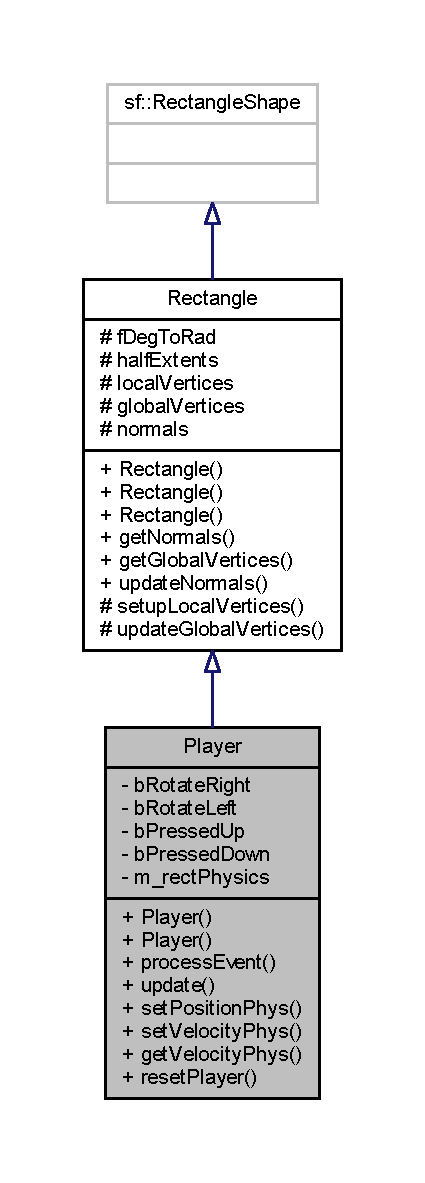
\includegraphics[height=550pt]{class_player__inherit__graph}
\end{center}
\end{figure}


Collaboration diagram for Player\+:\nopagebreak
\begin{figure}[H]
\begin{center}
\leavevmode
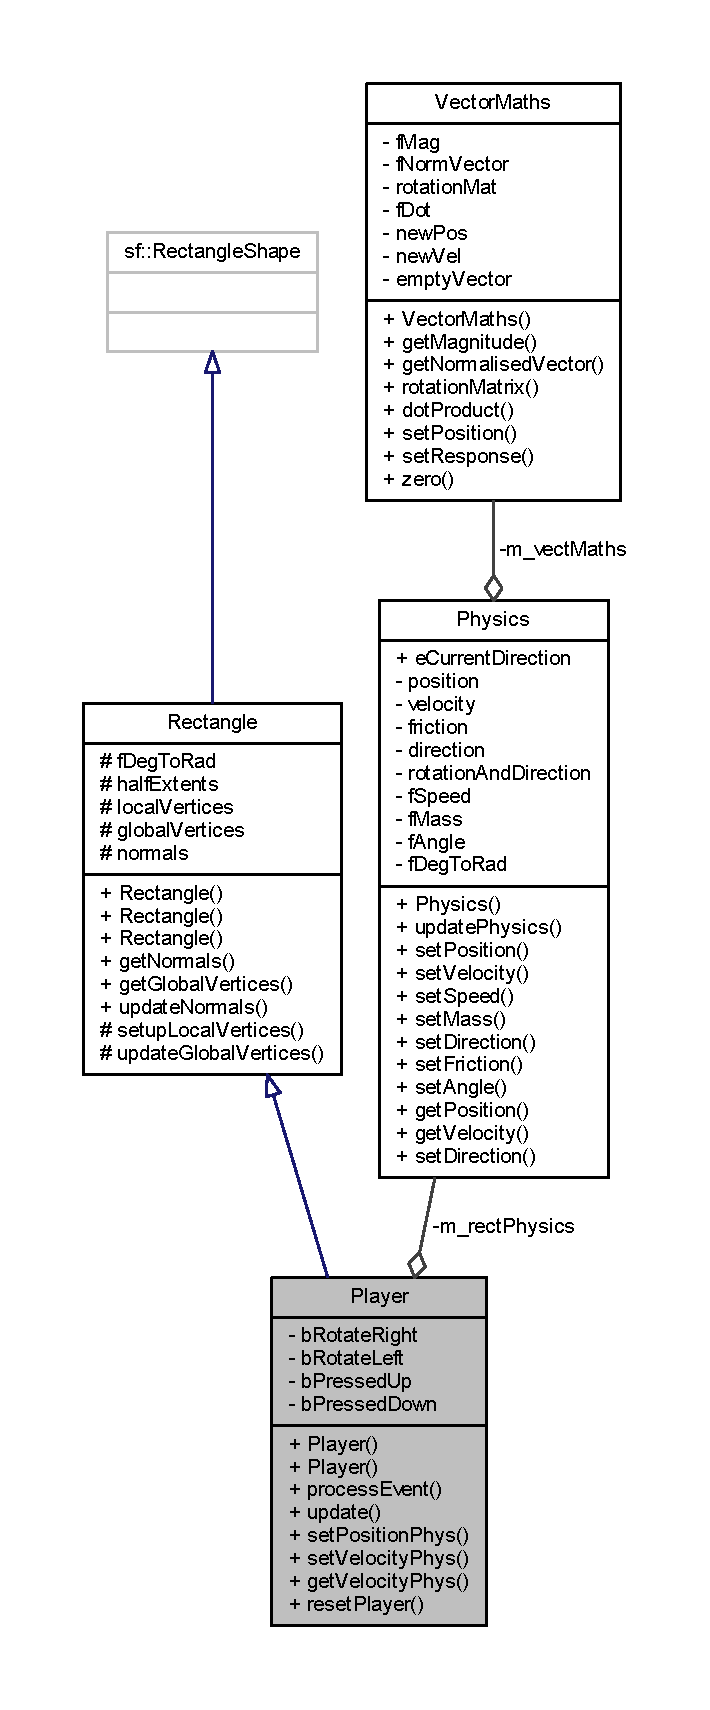
\includegraphics[height=550pt]{class_player__coll__graph}
\end{center}
\end{figure}
\subsection*{Public Member Functions}
\begin{DoxyCompactItemize}
\item 
\hyperlink{class_player_affe0cc3cb714f6deb4e62f0c0d3f1fd8}{Player} ()
\item 
\hyperlink{class_player_af325f67103c14661d1dbc133bd066aad}{Player} (sf\+::\+Vector2f \&position, sf\+::\+Vector2f \&dimensions, sf\+::\+Texture \&texture)
\item 
void \hyperlink{class_player_a2adec8ca29f3ab52362174ccd1ed7d4d}{process\+Event} (sf\+::\+Event \&e)
\item 
void \hyperlink{class_player_a480140d0e89332be296673e63433c76a}{update} (float time\+Step)
\item 
void \hyperlink{class_player_afda87686c6028869242b8938fc98c936}{set\+Position\+Phys} (sf\+::\+Vector2f other)
\item 
void \hyperlink{class_player_ad0f9460e27f4d32e4326def511514688}{set\+Velocity\+Phys} (sf\+::\+Vector2f other)
\item 
sf\+::\+Vector2f \hyperlink{class_player_a2dbb7781b7ce5c32d3a0d0b4db2d2eb0}{get\+Velocity\+Phys} ()
\item 
void \hyperlink{class_player_a64f3efd0c43b7aa3138d532ff8dc615a}{reset\+Player} ()
\end{DoxyCompactItemize}
\subsection*{Private Attributes}
\begin{DoxyCompactItemize}
\item 
bool \hyperlink{class_player_ab898f2f67f989df21804ecb72f4d25b1}{b\+Rotate\+Right}
\item 
bool \hyperlink{class_player_ae2fd38e391d041ade292c8fd2a417f4f}{b\+Rotate\+Left}
\item 
bool \hyperlink{class_player_ad00b7a7e4920b62e13c152a2374c66dd}{b\+Pressed\+Up}
\item 
bool \hyperlink{class_player_aa195c952c7b5f09f59ed32935c8ed111}{b\+Pressed\+Down}
\item 
\hyperlink{class_physics}{Physics} \hyperlink{class_player_adc5a0f2ba8dd25317f817e4f65de9cae}{m\+\_\+rect\+Physics}
\end{DoxyCompactItemize}
\subsection*{Additional Inherited Members}


\subsection{Detailed Description}
This class is used to create and control a player. 

\subsection{Constructor \& Destructor Documentation}
\index{Player@{Player}!Player@{Player}}
\index{Player@{Player}!Player@{Player}}
\subsubsection[{\texorpdfstring{Player()}{Player()}}]{\setlength{\rightskip}{0pt plus 5cm}Player\+::\+Player (
\begin{DoxyParamCaption}
{}
\end{DoxyParamCaption}
)\hspace{0.3cm}{\ttfamily [inline]}}\hypertarget{class_player_affe0cc3cb714f6deb4e62f0c0d3f1fd8}{}\label{class_player_affe0cc3cb714f6deb4e62f0c0d3f1fd8}
Initializer. 

Here is the call graph for this function\+:\nopagebreak
\begin{figure}[H]
\begin{center}
\leavevmode
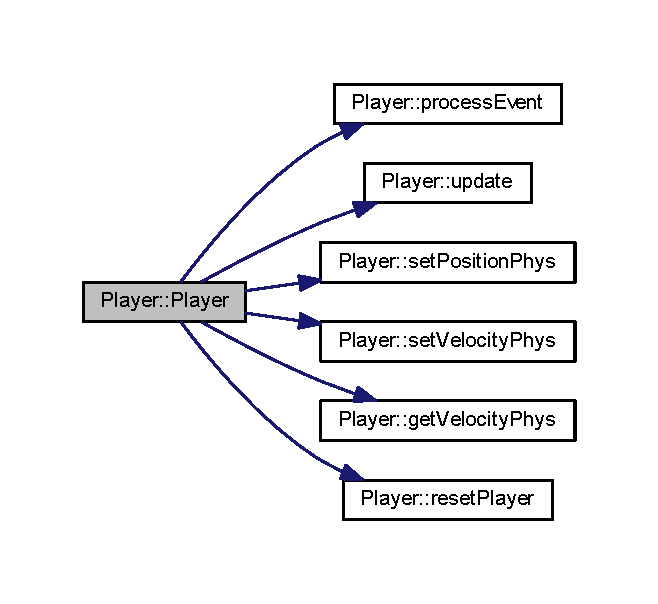
\includegraphics[width=316pt]{class_player_affe0cc3cb714f6deb4e62f0c0d3f1fd8_cgraph}
\end{center}
\end{figure}


\index{Player@{Player}!Player@{Player}}
\index{Player@{Player}!Player@{Player}}
\subsubsection[{\texorpdfstring{Player(sf\+::\+Vector2f \&position, sf\+::\+Vector2f \&dimensions, sf\+::\+Texture \&texture)}{Player(sf::Vector2f &position, sf::Vector2f &dimensions, sf::Texture &texture)}}]{\setlength{\rightskip}{0pt plus 5cm}Player\+::\+Player (
\begin{DoxyParamCaption}
\item[{sf\+::\+Vector2f \&}]{position, }
\item[{sf\+::\+Vector2f \&}]{dimensions, }
\item[{sf\+::\+Texture \&}]{texture}
\end{DoxyParamCaption}
)}\hypertarget{class_player_af325f67103c14661d1dbc133bd066aad}{}\label{class_player_af325f67103c14661d1dbc133bd066aad}
Constructor. 
\begin{DoxyParams}{Parameters}
{\em position} & = Position of the player. \\
\hline
{\em dimensions} & = Size of the player. \\
\hline
{\em texture} & = Texture to load. \\
\hline
\end{DoxyParams}


\subsection{Member Function Documentation}
\index{Player@{Player}!get\+Velocity\+Phys@{get\+Velocity\+Phys}}
\index{get\+Velocity\+Phys@{get\+Velocity\+Phys}!Player@{Player}}
\subsubsection[{\texorpdfstring{get\+Velocity\+Phys()}{getVelocityPhys()}}]{\setlength{\rightskip}{0pt plus 5cm}sf\+::\+Vector2f Player\+::get\+Velocity\+Phys (
\begin{DoxyParamCaption}
{}
\end{DoxyParamCaption}
)}\hypertarget{class_player_a2dbb7781b7ce5c32d3a0d0b4db2d2eb0}{}\label{class_player_a2dbb7781b7ce5c32d3a0d0b4db2d2eb0}
Returns a velocity vector. \begin{DoxyReturn}{Returns}
m\+\_\+rect\+Physics.\+get\+Velocity() = Returns a current velocity vector. 
\end{DoxyReturn}
\index{Player@{Player}!process\+Event@{process\+Event}}
\index{process\+Event@{process\+Event}!Player@{Player}}
\subsubsection[{\texorpdfstring{process\+Event(sf\+::\+Event \&e)}{processEvent(sf::Event &e)}}]{\setlength{\rightskip}{0pt plus 5cm}void Player\+::process\+Event (
\begin{DoxyParamCaption}
\item[{sf\+::\+Event \&}]{e}
\end{DoxyParamCaption}
)}\hypertarget{class_player_a2adec8ca29f3ab52362174ccd1ed7d4d}{}\label{class_player_a2adec8ca29f3ab52362174ccd1ed7d4d}
Process any key events. 
\begin{DoxyParams}{Parameters}
{\em e} & = Event variable needed to capture any key presses. \\
\hline
\end{DoxyParams}
\index{Player@{Player}!reset\+Player@{reset\+Player}}
\index{reset\+Player@{reset\+Player}!Player@{Player}}
\subsubsection[{\texorpdfstring{reset\+Player()}{resetPlayer()}}]{\setlength{\rightskip}{0pt plus 5cm}void Player\+::reset\+Player (
\begin{DoxyParamCaption}
{}
\end{DoxyParamCaption}
)}\hypertarget{class_player_a64f3efd0c43b7aa3138d532ff8dc615a}{}\label{class_player_a64f3efd0c43b7aa3138d532ff8dc615a}
Resets player\textquotesingle{}s variables. \index{Player@{Player}!set\+Position\+Phys@{set\+Position\+Phys}}
\index{set\+Position\+Phys@{set\+Position\+Phys}!Player@{Player}}
\subsubsection[{\texorpdfstring{set\+Position\+Phys(sf\+::\+Vector2f other)}{setPositionPhys(sf::Vector2f other)}}]{\setlength{\rightskip}{0pt plus 5cm}void Player\+::set\+Position\+Phys (
\begin{DoxyParamCaption}
\item[{sf\+::\+Vector2f}]{other}
\end{DoxyParamCaption}
)}\hypertarget{class_player_afda87686c6028869242b8938fc98c936}{}\label{class_player_afda87686c6028869242b8938fc98c936}
Sets a position of the player for physics. 
\begin{DoxyParams}{Parameters}
{\em other} & = New position vector. \\
\hline
\end{DoxyParams}
\index{Player@{Player}!set\+Velocity\+Phys@{set\+Velocity\+Phys}}
\index{set\+Velocity\+Phys@{set\+Velocity\+Phys}!Player@{Player}}
\subsubsection[{\texorpdfstring{set\+Velocity\+Phys(sf\+::\+Vector2f other)}{setVelocityPhys(sf::Vector2f other)}}]{\setlength{\rightskip}{0pt plus 5cm}void Player\+::set\+Velocity\+Phys (
\begin{DoxyParamCaption}
\item[{sf\+::\+Vector2f}]{other}
\end{DoxyParamCaption}
)}\hypertarget{class_player_ad0f9460e27f4d32e4326def511514688}{}\label{class_player_ad0f9460e27f4d32e4326def511514688}
Sets a velocity of the player for physics. 
\begin{DoxyParams}{Parameters}
{\em other} & = New velocity vector. \\
\hline
\end{DoxyParams}
\index{Player@{Player}!update@{update}}
\index{update@{update}!Player@{Player}}
\subsubsection[{\texorpdfstring{update(float time\+Step)}{update(float timeStep)}}]{\setlength{\rightskip}{0pt plus 5cm}void Player\+::update (
\begin{DoxyParamCaption}
\item[{float}]{time\+Step}
\end{DoxyParamCaption}
)}\hypertarget{class_player_a480140d0e89332be296673e63433c76a}{}\label{class_player_a480140d0e89332be296673e63433c76a}
Updates the player. 
\begin{DoxyParams}{Parameters}
{\em time\+Step} & = Time which updates most of the functions and variables, for example velocity. \\
\hline
\end{DoxyParams}


\subsection{Member Data Documentation}
\index{Player@{Player}!b\+Pressed\+Down@{b\+Pressed\+Down}}
\index{b\+Pressed\+Down@{b\+Pressed\+Down}!Player@{Player}}
\subsubsection[{\texorpdfstring{b\+Pressed\+Down}{bPressedDown}}]{\setlength{\rightskip}{0pt plus 5cm}bool Player\+::b\+Pressed\+Down\hspace{0.3cm}{\ttfamily [private]}}\hypertarget{class_player_aa195c952c7b5f09f59ed32935c8ed111}{}\label{class_player_aa195c952c7b5f09f59ed32935c8ed111}
Confirmation to go down. \index{Player@{Player}!b\+Pressed\+Up@{b\+Pressed\+Up}}
\index{b\+Pressed\+Up@{b\+Pressed\+Up}!Player@{Player}}
\subsubsection[{\texorpdfstring{b\+Pressed\+Up}{bPressedUp}}]{\setlength{\rightskip}{0pt plus 5cm}bool Player\+::b\+Pressed\+Up\hspace{0.3cm}{\ttfamily [private]}}\hypertarget{class_player_ad00b7a7e4920b62e13c152a2374c66dd}{}\label{class_player_ad00b7a7e4920b62e13c152a2374c66dd}
Confirmation to go up. \index{Player@{Player}!b\+Rotate\+Left@{b\+Rotate\+Left}}
\index{b\+Rotate\+Left@{b\+Rotate\+Left}!Player@{Player}}
\subsubsection[{\texorpdfstring{b\+Rotate\+Left}{bRotateLeft}}]{\setlength{\rightskip}{0pt plus 5cm}bool Player\+::b\+Rotate\+Left\hspace{0.3cm}{\ttfamily [private]}}\hypertarget{class_player_ae2fd38e391d041ade292c8fd2a417f4f}{}\label{class_player_ae2fd38e391d041ade292c8fd2a417f4f}
Confirmation to rotate left. \index{Player@{Player}!b\+Rotate\+Right@{b\+Rotate\+Right}}
\index{b\+Rotate\+Right@{b\+Rotate\+Right}!Player@{Player}}
\subsubsection[{\texorpdfstring{b\+Rotate\+Right}{bRotateRight}}]{\setlength{\rightskip}{0pt plus 5cm}bool Player\+::b\+Rotate\+Right\hspace{0.3cm}{\ttfamily [private]}}\hypertarget{class_player_ab898f2f67f989df21804ecb72f4d25b1}{}\label{class_player_ab898f2f67f989df21804ecb72f4d25b1}
Confirmation to rotate right. \index{Player@{Player}!m\+\_\+rect\+Physics@{m\+\_\+rect\+Physics}}
\index{m\+\_\+rect\+Physics@{m\+\_\+rect\+Physics}!Player@{Player}}
\subsubsection[{\texorpdfstring{m\+\_\+rect\+Physics}{m_rectPhysics}}]{\setlength{\rightskip}{0pt plus 5cm}{\bf Physics} Player\+::m\+\_\+rect\+Physics\hspace{0.3cm}{\ttfamily [private]}}\hypertarget{class_player_adc5a0f2ba8dd25317f817e4f65de9cae}{}\label{class_player_adc5a0f2ba8dd25317f817e4f65de9cae}
\hyperlink{class_physics}{Physics} for the player. 

The documentation for this class was generated from the following file\+:\begin{DoxyCompactItemize}
\item 
include/\hyperlink{player_8h}{player.\+h}\end{DoxyCompactItemize}

\hypertarget{class_rectangle}{}\section{Rectangle Class Reference}
\label{class_rectangle}\index{Rectangle@{Rectangle}}


This class is used to create an abstract base class of the rectangle.  




{\ttfamily \#include $<$rectangle.\+h$>$}



Inheritance diagram for Rectangle\+:\nopagebreak
\begin{figure}[H]
\begin{center}
\leavevmode
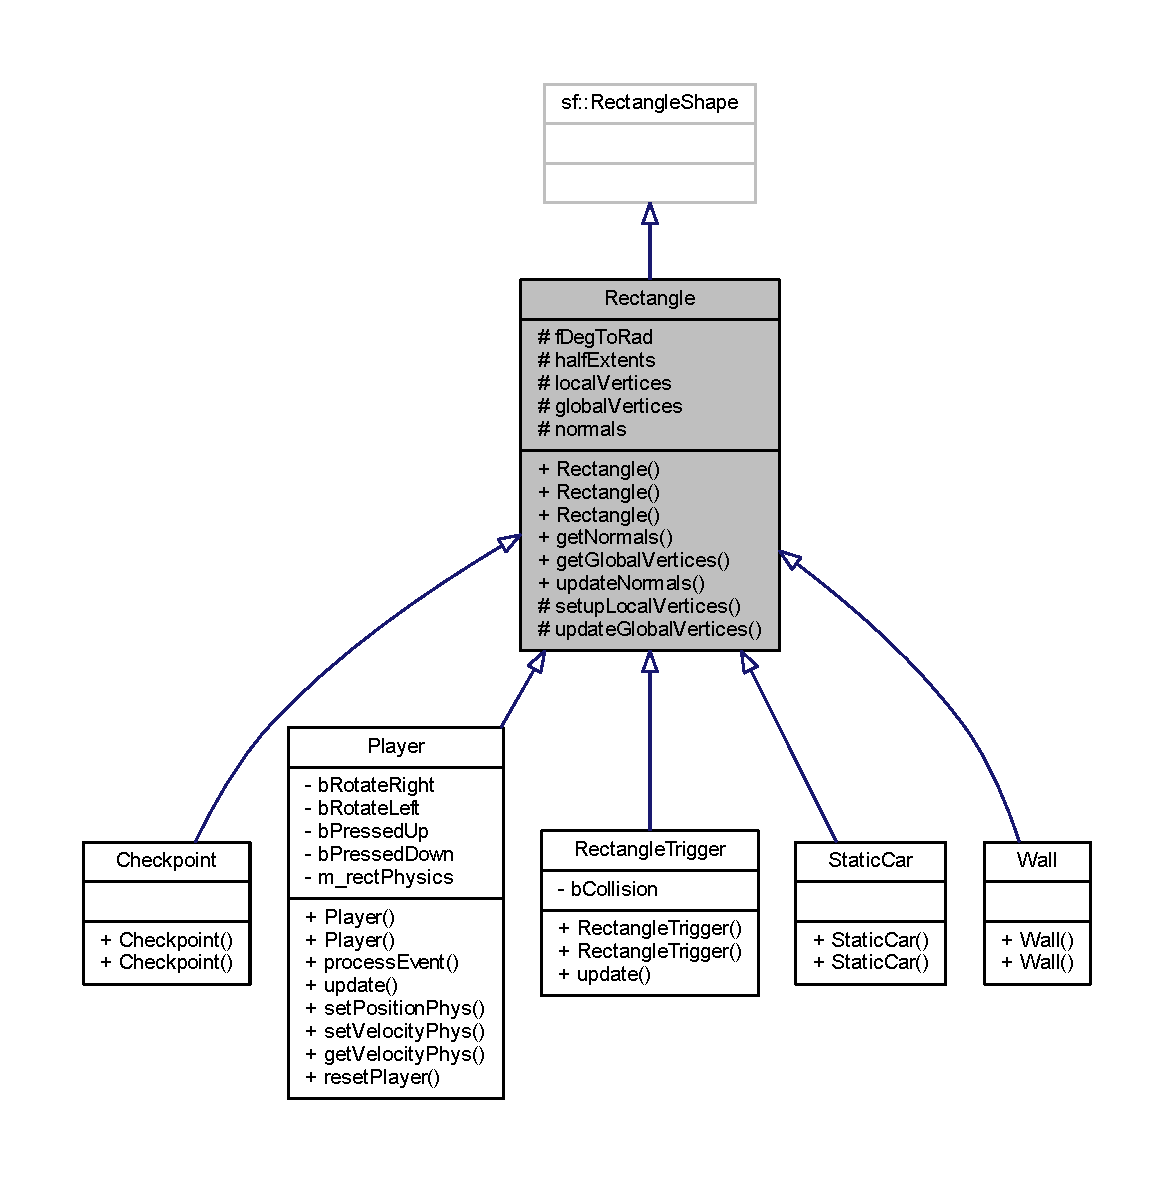
\includegraphics[width=350pt]{class_rectangle__inherit__graph}
\end{center}
\end{figure}


Collaboration diagram for Rectangle\+:\nopagebreak
\begin{figure}[H]
\begin{center}
\leavevmode
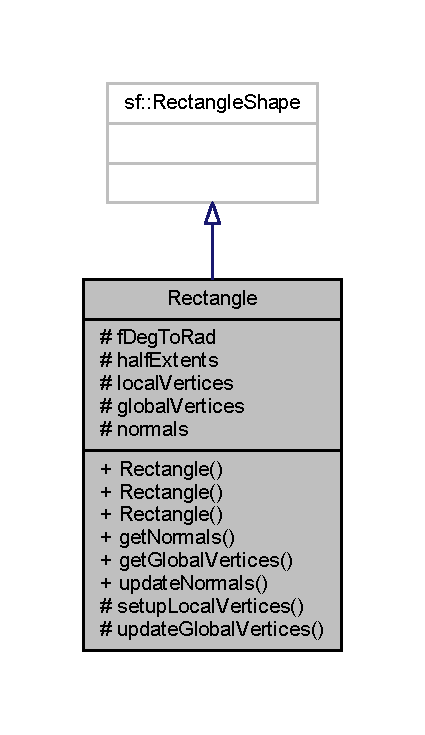
\includegraphics[width=204pt]{class_rectangle__coll__graph}
\end{center}
\end{figure}
\subsection*{Public Member Functions}
\begin{DoxyCompactItemize}
\item 
\hyperlink{class_rectangle_a8a933e0ebd9e80ce91e61ffe87fd577e}{Rectangle} ()
\item 
\hyperlink{class_rectangle_af7d678fca8036bea351850af59a75a35}{Rectangle} (const sf\+::\+Vector2f \&position, const sf\+::\+Vector2f \&dimensions)
\item 
\hyperlink{class_rectangle_af7899b9fa819743228eaacd41b79a77c}{Rectangle} (const sf\+::\+Vector2f \&position, const sf\+::\+Vector2f \&dimensions, const sf\+::\+Texture \&texture)
\item 
std\+::vector$<$ sf\+::\+Vector2f $>$ \hyperlink{class_rectangle_ac1842f29ce2238f53aacb2027d7095b6}{get\+Normals} () const 
\item 
std\+::vector$<$ sf\+::\+Vertex $>$ \hyperlink{class_rectangle_ab8a7c003e34e8dfb8db4aafa2a76ea80}{get\+Global\+Vertices} () const 
\item 
void \hyperlink{class_rectangle_a8e9aa14262388a6dcaa4f7303b0ae9a7}{update\+Normals} (float rotation)
\end{DoxyCompactItemize}
\subsection*{Protected Member Functions}
\begin{DoxyCompactItemize}
\item 
void \hyperlink{class_rectangle_acc37caedf705dda800b5173caa09769d}{setup\+Local\+Vertices} ()
\item 
void \hyperlink{class_rectangle_aafbe42c32cdb58691faeb16d16c90f31}{update\+Global\+Vertices} (float rotation)
\end{DoxyCompactItemize}
\subsection*{Protected Attributes}
\begin{DoxyCompactItemize}
\item 
float \hyperlink{class_rectangle_aa0d46e31bf4f23436c267b05b4404341}{f\+Deg\+To\+Rad}
\begin{DoxyCompactList}\small\item\em (float)M\+\_\+\+PI / 180.\+f; \end{DoxyCompactList}\item 
sf\+::\+Vector2f \hyperlink{class_rectangle_aa51d214692884af3c403655d08d48076}{half\+Extents}
\item 
std\+::vector$<$ sf\+::\+Vertex $>$ \hyperlink{class_rectangle_a827fd01362a28eca0b1bb3f89c559d36}{local\+Vertices}
\item 
std\+::vector$<$ sf\+::\+Vertex $>$ \hyperlink{class_rectangle_a2231304da216c0c643bdffecdc514419}{global\+Vertices}
\item 
std\+::vector$<$ sf\+::\+Vector2f $>$ \hyperlink{class_rectangle_ac94537e97b66a5d92a1919c99543c598}{normals}
\end{DoxyCompactItemize}


\subsection{Detailed Description}
This class is used to create an abstract base class of the rectangle. 

\subsection{Constructor \& Destructor Documentation}
\index{Rectangle@{Rectangle}!Rectangle@{Rectangle}}
\index{Rectangle@{Rectangle}!Rectangle@{Rectangle}}
\subsubsection[{\texorpdfstring{Rectangle()}{Rectangle()}}]{\setlength{\rightskip}{0pt plus 5cm}Rectangle\+::\+Rectangle (
\begin{DoxyParamCaption}
{}
\end{DoxyParamCaption}
)\hspace{0.3cm}{\ttfamily [inline]}}\hypertarget{class_rectangle_a8a933e0ebd9e80ce91e61ffe87fd577e}{}\label{class_rectangle_a8a933e0ebd9e80ce91e61ffe87fd577e}
Initializer. 

Here is the call graph for this function\+:\nopagebreak
\begin{figure}[H]
\begin{center}
\leavevmode
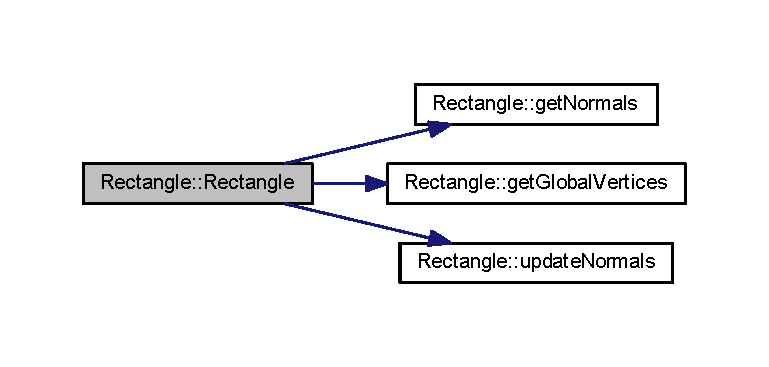
\includegraphics[width=350pt]{class_rectangle_a8a933e0ebd9e80ce91e61ffe87fd577e_cgraph}
\end{center}
\end{figure}


\index{Rectangle@{Rectangle}!Rectangle@{Rectangle}}
\index{Rectangle@{Rectangle}!Rectangle@{Rectangle}}
\subsubsection[{\texorpdfstring{Rectangle(const sf\+::\+Vector2f \&position, const sf\+::\+Vector2f \&dimensions)}{Rectangle(const sf::Vector2f &position, const sf::Vector2f &dimensions)}}]{\setlength{\rightskip}{0pt plus 5cm}Rectangle\+::\+Rectangle (
\begin{DoxyParamCaption}
\item[{const sf\+::\+Vector2f \&}]{position, }
\item[{const sf\+::\+Vector2f \&}]{dimensions}
\end{DoxyParamCaption}
)}\hypertarget{class_rectangle_af7d678fca8036bea351850af59a75a35}{}\label{class_rectangle_af7d678fca8036bea351850af59a75a35}
Constructor. 
\begin{DoxyParams}{Parameters}
{\em position} & = Position of the rectangle. \\
\hline
{\em dimensions} & = Size of the rectangle \\
\hline
\end{DoxyParams}
\index{Rectangle@{Rectangle}!Rectangle@{Rectangle}}
\index{Rectangle@{Rectangle}!Rectangle@{Rectangle}}
\subsubsection[{\texorpdfstring{Rectangle(const sf\+::\+Vector2f \&position, const sf\+::\+Vector2f \&dimensions, const sf\+::\+Texture \&texture)}{Rectangle(const sf::Vector2f &position, const sf::Vector2f &dimensions, const sf::Texture &texture)}}]{\setlength{\rightskip}{0pt plus 5cm}Rectangle\+::\+Rectangle (
\begin{DoxyParamCaption}
\item[{const sf\+::\+Vector2f \&}]{position, }
\item[{const sf\+::\+Vector2f \&}]{dimensions, }
\item[{const sf\+::\+Texture \&}]{texture}
\end{DoxyParamCaption}
)}\hypertarget{class_rectangle_af7899b9fa819743228eaacd41b79a77c}{}\label{class_rectangle_af7899b9fa819743228eaacd41b79a77c}
Constructor. 
\begin{DoxyParams}{Parameters}
{\em position} & = Position of the rectangle. \\
\hline
{\em dimensions} & = Size of the rectangle. \\
\hline
{\em texture} & = Texture to load. \\
\hline
\end{DoxyParams}


\subsection{Member Function Documentation}
\index{Rectangle@{Rectangle}!get\+Global\+Vertices@{get\+Global\+Vertices}}
\index{get\+Global\+Vertices@{get\+Global\+Vertices}!Rectangle@{Rectangle}}
\subsubsection[{\texorpdfstring{get\+Global\+Vertices() const }{getGlobalVertices() const }}]{\setlength{\rightskip}{0pt plus 5cm}std\+::vector$<$sf\+::\+Vertex$>$ Rectangle\+::get\+Global\+Vertices (
\begin{DoxyParamCaption}
{}
\end{DoxyParamCaption}
) const}\hypertarget{class_rectangle_ab8a7c003e34e8dfb8db4aafa2a76ea80}{}\label{class_rectangle_ab8a7c003e34e8dfb8db4aafa2a76ea80}
Returns global vertices of said rectangle. \begin{DoxyReturn}{Returns}
global\+Vertices = Returns global vertices of the rectangle. 
\end{DoxyReturn}
\index{Rectangle@{Rectangle}!get\+Normals@{get\+Normals}}
\index{get\+Normals@{get\+Normals}!Rectangle@{Rectangle}}
\subsubsection[{\texorpdfstring{get\+Normals() const }{getNormals() const }}]{\setlength{\rightskip}{0pt plus 5cm}std\+::vector$<$sf\+::\+Vector2f$>$ Rectangle\+::get\+Normals (
\begin{DoxyParamCaption}
{}
\end{DoxyParamCaption}
) const}\hypertarget{class_rectangle_ac1842f29ce2238f53aacb2027d7095b6}{}\label{class_rectangle_ac1842f29ce2238f53aacb2027d7095b6}
Returns normals of said rectangle. \begin{DoxyReturn}{Returns}
normals = Returns face normals of the rectangle. 
\end{DoxyReturn}
\index{Rectangle@{Rectangle}!setup\+Local\+Vertices@{setup\+Local\+Vertices}}
\index{setup\+Local\+Vertices@{setup\+Local\+Vertices}!Rectangle@{Rectangle}}
\subsubsection[{\texorpdfstring{setup\+Local\+Vertices()}{setupLocalVertices()}}]{\setlength{\rightskip}{0pt plus 5cm}void Rectangle\+::setup\+Local\+Vertices (
\begin{DoxyParamCaption}
{}
\end{DoxyParamCaption}
)\hspace{0.3cm}{\ttfamily [protected]}}\hypertarget{class_rectangle_acc37caedf705dda800b5173caa09769d}{}\label{class_rectangle_acc37caedf705dda800b5173caa09769d}
One time setup of the local vertices. \index{Rectangle@{Rectangle}!update\+Global\+Vertices@{update\+Global\+Vertices}}
\index{update\+Global\+Vertices@{update\+Global\+Vertices}!Rectangle@{Rectangle}}
\subsubsection[{\texorpdfstring{update\+Global\+Vertices(float rotation)}{updateGlobalVertices(float rotation)}}]{\setlength{\rightskip}{0pt plus 5cm}void Rectangle\+::update\+Global\+Vertices (
\begin{DoxyParamCaption}
\item[{float}]{rotation}
\end{DoxyParamCaption}
)\hspace{0.3cm}{\ttfamily [protected]}}\hypertarget{class_rectangle_aafbe42c32cdb58691faeb16d16c90f31}{}\label{class_rectangle_aafbe42c32cdb58691faeb16d16c90f31}
One time setup of the global vertices including rotation. \index{Rectangle@{Rectangle}!update\+Normals@{update\+Normals}}
\index{update\+Normals@{update\+Normals}!Rectangle@{Rectangle}}
\subsubsection[{\texorpdfstring{update\+Normals(float rotation)}{updateNormals(float rotation)}}]{\setlength{\rightskip}{0pt plus 5cm}void Rectangle\+::update\+Normals (
\begin{DoxyParamCaption}
\item[{float}]{rotation}
\end{DoxyParamCaption}
)}\hypertarget{class_rectangle_a8e9aa14262388a6dcaa4f7303b0ae9a7}{}\label{class_rectangle_a8e9aa14262388a6dcaa4f7303b0ae9a7}
Updates face normals based on the given rotation. 
\begin{DoxyParams}{Parameters}
{\em rotation} & = Rotation needed so that normals can be updated whenever the rectangle rotates. \\
\hline
\end{DoxyParams}


\subsection{Member Data Documentation}
\index{Rectangle@{Rectangle}!f\+Deg\+To\+Rad@{f\+Deg\+To\+Rad}}
\index{f\+Deg\+To\+Rad@{f\+Deg\+To\+Rad}!Rectangle@{Rectangle}}
\subsubsection[{\texorpdfstring{f\+Deg\+To\+Rad}{fDegToRad}}]{\setlength{\rightskip}{0pt plus 5cm}float Rectangle\+::f\+Deg\+To\+Rad\hspace{0.3cm}{\ttfamily [protected]}}\hypertarget{class_rectangle_aa0d46e31bf4f23436c267b05b4404341}{}\label{class_rectangle_aa0d46e31bf4f23436c267b05b4404341}


(float)M\+\_\+\+PI / 180.\+f; 

Formula converting degrees to radians. \index{Rectangle@{Rectangle}!global\+Vertices@{global\+Vertices}}
\index{global\+Vertices@{global\+Vertices}!Rectangle@{Rectangle}}
\subsubsection[{\texorpdfstring{global\+Vertices}{globalVertices}}]{\setlength{\rightskip}{0pt plus 5cm}std\+::vector$<$sf\+::\+Vertex$>$ Rectangle\+::global\+Vertices\hspace{0.3cm}{\ttfamily [protected]}}\hypertarget{class_rectangle_a2231304da216c0c643bdffecdc514419}{}\label{class_rectangle_a2231304da216c0c643bdffecdc514419}
Global vertices of the rectangle. \index{Rectangle@{Rectangle}!half\+Extents@{half\+Extents}}
\index{half\+Extents@{half\+Extents}!Rectangle@{Rectangle}}
\subsubsection[{\texorpdfstring{half\+Extents}{halfExtents}}]{\setlength{\rightskip}{0pt plus 5cm}sf\+::\+Vector2f Rectangle\+::half\+Extents\hspace{0.3cm}{\ttfamily [protected]}}\hypertarget{class_rectangle_aa51d214692884af3c403655d08d48076}{}\label{class_rectangle_aa51d214692884af3c403655d08d48076}
Half extents needed to declare vertices. \index{Rectangle@{Rectangle}!local\+Vertices@{local\+Vertices}}
\index{local\+Vertices@{local\+Vertices}!Rectangle@{Rectangle}}
\subsubsection[{\texorpdfstring{local\+Vertices}{localVertices}}]{\setlength{\rightskip}{0pt plus 5cm}std\+::vector$<$sf\+::\+Vertex$>$ Rectangle\+::local\+Vertices\hspace{0.3cm}{\ttfamily [protected]}}\hypertarget{class_rectangle_a827fd01362a28eca0b1bb3f89c559d36}{}\label{class_rectangle_a827fd01362a28eca0b1bb3f89c559d36}
Local vertices of the rectangle. \index{Rectangle@{Rectangle}!normals@{normals}}
\index{normals@{normals}!Rectangle@{Rectangle}}
\subsubsection[{\texorpdfstring{normals}{normals}}]{\setlength{\rightskip}{0pt plus 5cm}std\+::vector$<$sf\+::\+Vector2f$>$ Rectangle\+::normals\hspace{0.3cm}{\ttfamily [protected]}}\hypertarget{class_rectangle_ac94537e97b66a5d92a1919c99543c598}{}\label{class_rectangle_ac94537e97b66a5d92a1919c99543c598}
Face normals of the rectangle. 

The documentation for this class was generated from the following file\+:\begin{DoxyCompactItemize}
\item 
include/\hyperlink{rectangle_8h}{rectangle.\+h}\end{DoxyCompactItemize}

\hypertarget{class_rectangle_trigger}{}\section{Rectangle\+Trigger Class Reference}
\label{class_rectangle_trigger}\index{Rectangle\+Trigger@{Rectangle\+Trigger}}


This class is used to create a trigger.  




{\ttfamily \#include $<$rectangle\+Trigger.\+h$>$}



Inheritance diagram for Rectangle\+Trigger\+:\nopagebreak
\begin{figure}[H]
\begin{center}
\leavevmode
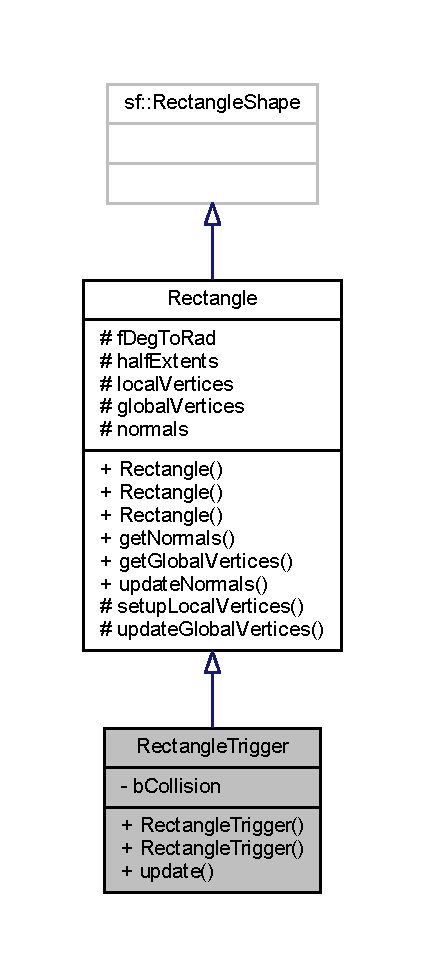
\includegraphics[width=204pt]{class_rectangle_trigger__inherit__graph}
\end{center}
\end{figure}


Collaboration diagram for Rectangle\+Trigger\+:\nopagebreak
\begin{figure}[H]
\begin{center}
\leavevmode
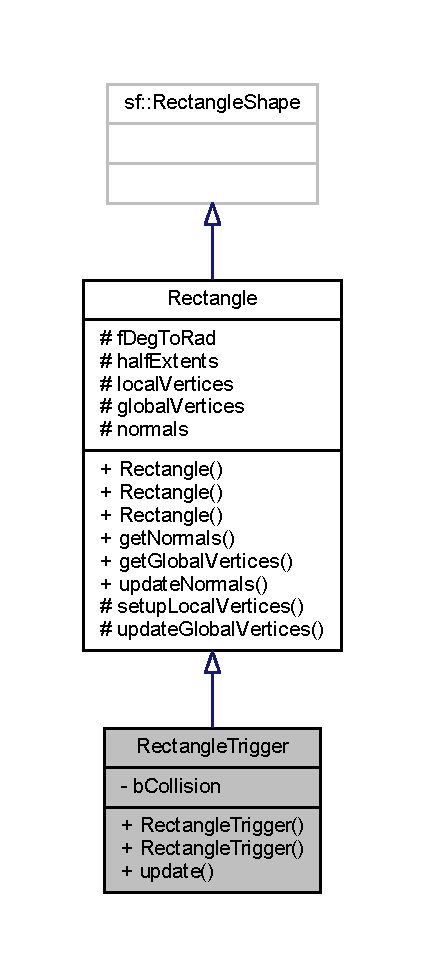
\includegraphics[width=204pt]{class_rectangle_trigger__coll__graph}
\end{center}
\end{figure}
\subsection*{Public Member Functions}
\begin{DoxyCompactItemize}
\item 
\hyperlink{class_rectangle_trigger_aee7b31c4083d365353ec11edba982417}{Rectangle\+Trigger} ()
\item 
\hyperlink{class_rectangle_trigger_ad607c4f7b40934e843ddeeca15ae4f57}{Rectangle\+Trigger} (const sf\+::\+Vector2f \&position, const sf\+::\+Vector2f \&dimensions, const float f\+Angle)
\item 
void \hyperlink{class_rectangle_trigger_ab82d08742d6adba94ec85e77914e0133}{update} (sf\+::\+Vector2f position, bool b\+Vertices)
\end{DoxyCompactItemize}
\subsection*{Private Attributes}
\begin{DoxyCompactItemize}
\item 
bool \hyperlink{class_rectangle_trigger_af6349342536e699e721edda955df97ce}{b\+Collision}
\end{DoxyCompactItemize}
\subsection*{Additional Inherited Members}


\subsection{Detailed Description}
This class is used to create a trigger. 

\subsection{Constructor \& Destructor Documentation}
\index{Rectangle\+Trigger@{Rectangle\+Trigger}!Rectangle\+Trigger@{Rectangle\+Trigger}}
\index{Rectangle\+Trigger@{Rectangle\+Trigger}!Rectangle\+Trigger@{Rectangle\+Trigger}}
\subsubsection[{\texorpdfstring{Rectangle\+Trigger()}{RectangleTrigger()}}]{\setlength{\rightskip}{0pt plus 5cm}Rectangle\+Trigger\+::\+Rectangle\+Trigger (
\begin{DoxyParamCaption}
{}
\end{DoxyParamCaption}
)\hspace{0.3cm}{\ttfamily [inline]}}\hypertarget{class_rectangle_trigger_aee7b31c4083d365353ec11edba982417}{}\label{class_rectangle_trigger_aee7b31c4083d365353ec11edba982417}
Initializer. 

Here is the call graph for this function\+:\nopagebreak
\begin{figure}[H]
\begin{center}
\leavevmode
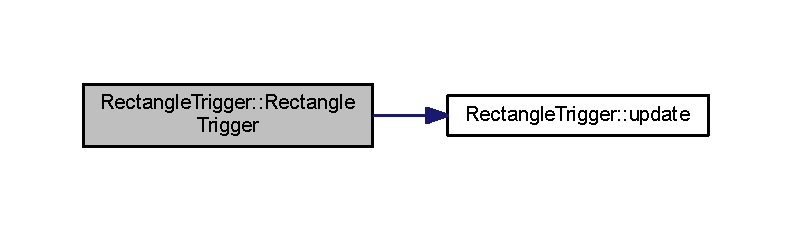
\includegraphics[width=350pt]{class_rectangle_trigger_aee7b31c4083d365353ec11edba982417_cgraph}
\end{center}
\end{figure}


\index{Rectangle\+Trigger@{Rectangle\+Trigger}!Rectangle\+Trigger@{Rectangle\+Trigger}}
\index{Rectangle\+Trigger@{Rectangle\+Trigger}!Rectangle\+Trigger@{Rectangle\+Trigger}}
\subsubsection[{\texorpdfstring{Rectangle\+Trigger(const sf\+::\+Vector2f \&position, const sf\+::\+Vector2f \&dimensions, const float f\+Angle)}{RectangleTrigger(const sf::Vector2f &position, const sf::Vector2f &dimensions, const float fAngle)}}]{\setlength{\rightskip}{0pt plus 5cm}Rectangle\+Trigger\+::\+Rectangle\+Trigger (
\begin{DoxyParamCaption}
\item[{const sf\+::\+Vector2f \&}]{position, }
\item[{const sf\+::\+Vector2f \&}]{dimensions, }
\item[{const float}]{f\+Angle}
\end{DoxyParamCaption}
)}\hypertarget{class_rectangle_trigger_ad607c4f7b40934e843ddeeca15ae4f57}{}\label{class_rectangle_trigger_ad607c4f7b40934e843ddeeca15ae4f57}
Constructor. 
\begin{DoxyParams}{Parameters}
{\em position} & = Position of the rectangle. \\
\hline
{\em dimensions} & = Size of the rectangle. \\
\hline
{\em f\+Angle} & = An orientation of the trigger \\
\hline
\end{DoxyParams}


\subsection{Member Function Documentation}
\index{Rectangle\+Trigger@{Rectangle\+Trigger}!update@{update}}
\index{update@{update}!Rectangle\+Trigger@{Rectangle\+Trigger}}
\subsubsection[{\texorpdfstring{update(sf\+::\+Vector2f position, bool b\+Vertices)}{update(sf::Vector2f position, bool bVertices)}}]{\setlength{\rightskip}{0pt plus 5cm}void Rectangle\+Trigger\+::update (
\begin{DoxyParamCaption}
\item[{sf\+::\+Vector2f}]{position, }
\item[{bool}]{b\+Vertices}
\end{DoxyParamCaption}
)}\hypertarget{class_rectangle_trigger_ab82d08742d6adba94ec85e77914e0133}{}\label{class_rectangle_trigger_ab82d08742d6adba94ec85e77914e0133}
\hyperlink{class_rectangle}{Rectangle} update. 
\begin{DoxyParams}{Parameters}
{\em position} & = Position that needs updating. \\
\hline
{\em b\+Vertices} & = Whether to update global vertices of the trigger \\
\hline
\end{DoxyParams}


\subsection{Member Data Documentation}
\index{Rectangle\+Trigger@{Rectangle\+Trigger}!b\+Collision@{b\+Collision}}
\index{b\+Collision@{b\+Collision}!Rectangle\+Trigger@{Rectangle\+Trigger}}
\subsubsection[{\texorpdfstring{b\+Collision}{bCollision}}]{\setlength{\rightskip}{0pt plus 5cm}bool Rectangle\+Trigger\+::b\+Collision\hspace{0.3cm}{\ttfamily [private]}}\hypertarget{class_rectangle_trigger_af6349342536e699e721edda955df97ce}{}\label{class_rectangle_trigger_af6349342536e699e721edda955df97ce}


The documentation for this class was generated from the following file\+:\begin{DoxyCompactItemize}
\item 
include/\hyperlink{rectangle_trigger_8h}{rectangle\+Trigger.\+h}\end{DoxyCompactItemize}

\hypertarget{class_simple_text}{}\section{Simple\+Text Class Reference}
\label{class_simple_text}\index{Simple\+Text@{Simple\+Text}}


This class is used to create a simple text on the screen.  




{\ttfamily \#include $<$simple\+Text.\+h$>$}



Inheritance diagram for Simple\+Text\+:\nopagebreak
\begin{figure}[H]
\begin{center}
\leavevmode
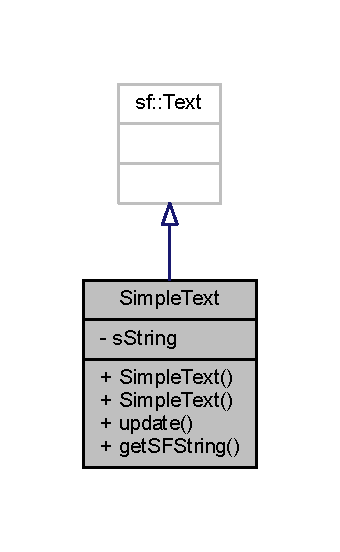
\includegraphics[width=163pt]{class_simple_text__inherit__graph}
\end{center}
\end{figure}


Collaboration diagram for Simple\+Text\+:\nopagebreak
\begin{figure}[H]
\begin{center}
\leavevmode
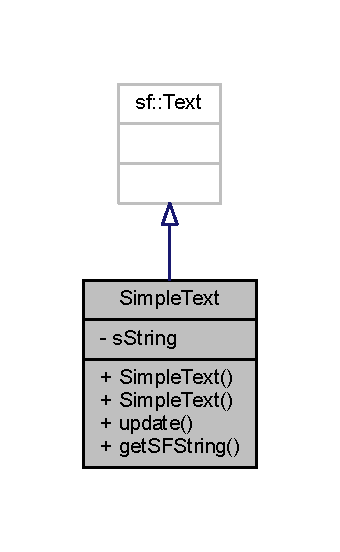
\includegraphics[width=163pt]{class_simple_text__coll__graph}
\end{center}
\end{figure}
\subsection*{Public Member Functions}
\begin{DoxyCompactItemize}
\item 
\hyperlink{class_simple_text_a29eb48751b83c726a2c335da508a6c98}{Simple\+Text} ()
\item 
\hyperlink{class_simple_text_a00514cf0f7f4e59e2ff9a7ba1f5fac89}{Simple\+Text} (sf\+::\+Vector2f \&position, sf\+::\+Font \&font, int i\+Size, sf\+::\+String string, sf\+::\+Color colour)
\item 
void \hyperlink{class_simple_text_a3441ec9de9d722e8d2e9a6f32292a2d3}{update} (sf\+::\+View \&view, float f\+PosX, float f\+PosY)
\item 
sf\+::\+String \hyperlink{class_simple_text_a6438f399a14826f80a058a88736c7f1e}{get\+S\+F\+String} ()
\end{DoxyCompactItemize}
\subsection*{Private Attributes}
\begin{DoxyCompactItemize}
\item 
sf\+::\+String \hyperlink{class_simple_text_a0b9fdb31761f017d7ecd0a81d234f1b1}{s\+String}
\end{DoxyCompactItemize}


\subsection{Detailed Description}
This class is used to create a simple text on the screen. 

\subsection{Constructor \& Destructor Documentation}
\index{Simple\+Text@{Simple\+Text}!Simple\+Text@{Simple\+Text}}
\index{Simple\+Text@{Simple\+Text}!Simple\+Text@{Simple\+Text}}
\subsubsection[{\texorpdfstring{Simple\+Text()}{SimpleText()}}]{\setlength{\rightskip}{0pt plus 5cm}Simple\+Text\+::\+Simple\+Text (
\begin{DoxyParamCaption}
{}
\end{DoxyParamCaption}
)\hspace{0.3cm}{\ttfamily [inline]}}\hypertarget{class_simple_text_a29eb48751b83c726a2c335da508a6c98}{}\label{class_simple_text_a29eb48751b83c726a2c335da508a6c98}
Initializer. 

Here is the call graph for this function\+:\nopagebreak
\begin{figure}[H]
\begin{center}
\leavevmode
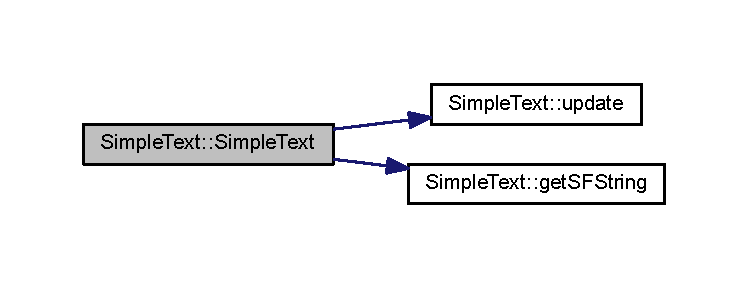
\includegraphics[width=350pt]{class_simple_text_a29eb48751b83c726a2c335da508a6c98_cgraph}
\end{center}
\end{figure}


\index{Simple\+Text@{Simple\+Text}!Simple\+Text@{Simple\+Text}}
\index{Simple\+Text@{Simple\+Text}!Simple\+Text@{Simple\+Text}}
\subsubsection[{\texorpdfstring{Simple\+Text(sf\+::\+Vector2f \&position, sf\+::\+Font \&font, int i\+Size, sf\+::\+String string, sf\+::\+Color colour)}{SimpleText(sf::Vector2f &position, sf::Font &font, int iSize, sf::String string, sf::Color colour)}}]{\setlength{\rightskip}{0pt plus 5cm}Simple\+Text\+::\+Simple\+Text (
\begin{DoxyParamCaption}
\item[{sf\+::\+Vector2f \&}]{position, }
\item[{sf\+::\+Font \&}]{font, }
\item[{int}]{i\+Size, }
\item[{sf\+::\+String}]{string, }
\item[{sf\+::\+Color}]{colour}
\end{DoxyParamCaption}
)}\hypertarget{class_simple_text_a00514cf0f7f4e59e2ff9a7ba1f5fac89}{}\label{class_simple_text_a00514cf0f7f4e59e2ff9a7ba1f5fac89}
Constructor. 
\begin{DoxyParams}{Parameters}
{\em position} & = A position on the screen. \\
\hline
{\em font} & = A font to load in. \\
\hline
{\em i\+Size} & = Size of the characters. \\
\hline
{\em string} & = A string to display. \\
\hline
{\em colour} & = Colour of the text. \\
\hline
\end{DoxyParams}


\subsection{Member Function Documentation}
\index{Simple\+Text@{Simple\+Text}!get\+S\+F\+String@{get\+S\+F\+String}}
\index{get\+S\+F\+String@{get\+S\+F\+String}!Simple\+Text@{Simple\+Text}}
\subsubsection[{\texorpdfstring{get\+S\+F\+String()}{getSFString()}}]{\setlength{\rightskip}{0pt plus 5cm}sf\+::\+String Simple\+Text\+::get\+S\+F\+String (
\begin{DoxyParamCaption}
{}
\end{DoxyParamCaption}
)}\hypertarget{class_simple_text_a6438f399a14826f80a058a88736c7f1e}{}\label{class_simple_text_a6438f399a14826f80a058a88736c7f1e}
Returns a sfml string type. \begin{DoxyReturn}{Returns}
s\+String 
\end{DoxyReturn}
\index{Simple\+Text@{Simple\+Text}!update@{update}}
\index{update@{update}!Simple\+Text@{Simple\+Text}}
\subsubsection[{\texorpdfstring{update(sf\+::\+View \&view, float f\+Pos\+X, float f\+Pos\+Y)}{update(sf::View &view, float fPosX, float fPosY)}}]{\setlength{\rightskip}{0pt plus 5cm}void Simple\+Text\+::update (
\begin{DoxyParamCaption}
\item[{sf\+::\+View \&}]{view, }
\item[{float}]{f\+PosX, }
\item[{float}]{f\+PosY}
\end{DoxyParamCaption}
)}\hypertarget{class_simple_text_a3441ec9de9d722e8d2e9a6f32292a2d3}{}\label{class_simple_text_a3441ec9de9d722e8d2e9a6f32292a2d3}
Updates the text. 
\begin{DoxyParams}{Parameters}
{\em view} & = A view that we will use to update our text position. \\
\hline
{\em f\+PosX} & = X position. You can add or subtract from the view.\+get\+Center().x. \\
\hline
{\em f\+PosY} & = Y position. You can add or subtract from the view.\+get\+Center().y. \\
\hline
\end{DoxyParams}


\subsection{Member Data Documentation}
\index{Simple\+Text@{Simple\+Text}!s\+String@{s\+String}}
\index{s\+String@{s\+String}!Simple\+Text@{Simple\+Text}}
\subsubsection[{\texorpdfstring{s\+String}{sString}}]{\setlength{\rightskip}{0pt plus 5cm}sf\+::\+String Simple\+Text\+::s\+String\hspace{0.3cm}{\ttfamily [private]}}\hypertarget{class_simple_text_a0b9fdb31761f017d7ecd0a81d234f1b1}{}\label{class_simple_text_a0b9fdb31761f017d7ecd0a81d234f1b1}
A string type from sfml. 

The documentation for this class was generated from the following file\+:\begin{DoxyCompactItemize}
\item 
include/\hyperlink{simple_text_8h}{simple\+Text.\+h}\end{DoxyCompactItemize}

\hypertarget{class_sphere_trigger}{}\section{Sphere\+Trigger Class Reference}
\label{class_sphere_trigger}\index{Sphere\+Trigger@{Sphere\+Trigger}}


This class is used to create a trigger.  




{\ttfamily \#include $<$sphere\+Trigger.\+h$>$}



Inheritance diagram for Sphere\+Trigger\+:\nopagebreak
\begin{figure}[H]
\begin{center}
\leavevmode
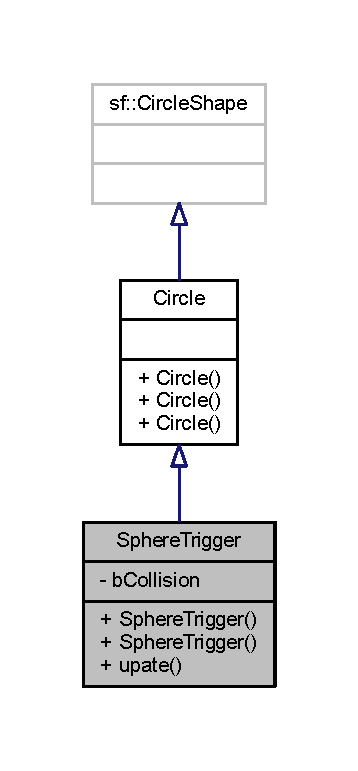
\includegraphics[width=172pt]{class_sphere_trigger__inherit__graph}
\end{center}
\end{figure}


Collaboration diagram for Sphere\+Trigger\+:\nopagebreak
\begin{figure}[H]
\begin{center}
\leavevmode
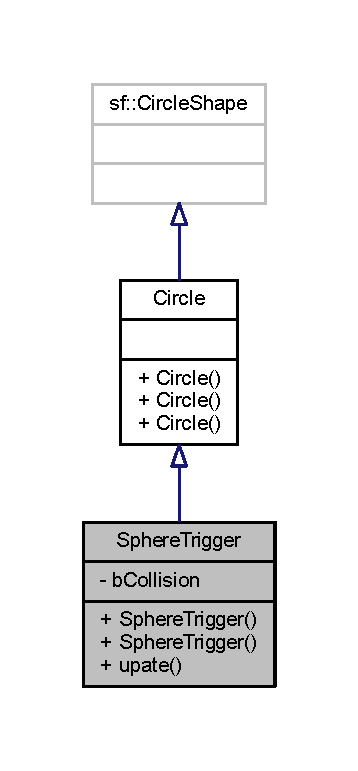
\includegraphics[width=172pt]{class_sphere_trigger__coll__graph}
\end{center}
\end{figure}
\subsection*{Public Member Functions}
\begin{DoxyCompactItemize}
\item 
\hyperlink{class_sphere_trigger_a4eddf434bac94055d32b0c5e37b24e0a}{Sphere\+Trigger} ()
\item 
\hyperlink{class_sphere_trigger_ac7dfa0626d77354df9e99dcfc23023ec}{Sphere\+Trigger} (const sf\+::\+Vector2f \&position, float f\+Radius)
\item 
void \hyperlink{class_sphere_trigger_af87f09551c86121cec4c9b0210de6166}{upate} (sf\+::\+Vector2f position)
\end{DoxyCompactItemize}
\subsection*{Private Attributes}
\begin{DoxyCompactItemize}
\item 
bool \hyperlink{class_sphere_trigger_aa2bbb652a3072e2041c75c01705486b9}{b\+Collision}
\end{DoxyCompactItemize}


\subsection{Detailed Description}
This class is used to create a trigger. 

\subsection{Constructor \& Destructor Documentation}
\index{Sphere\+Trigger@{Sphere\+Trigger}!Sphere\+Trigger@{Sphere\+Trigger}}
\index{Sphere\+Trigger@{Sphere\+Trigger}!Sphere\+Trigger@{Sphere\+Trigger}}
\subsubsection[{\texorpdfstring{Sphere\+Trigger()}{SphereTrigger()}}]{\setlength{\rightskip}{0pt plus 5cm}Sphere\+Trigger\+::\+Sphere\+Trigger (
\begin{DoxyParamCaption}
{}
\end{DoxyParamCaption}
)\hspace{0.3cm}{\ttfamily [inline]}}\hypertarget{class_sphere_trigger_a4eddf434bac94055d32b0c5e37b24e0a}{}\label{class_sphere_trigger_a4eddf434bac94055d32b0c5e37b24e0a}
Initializer. 

Here is the call graph for this function\+:\nopagebreak
\begin{figure}[H]
\begin{center}
\leavevmode
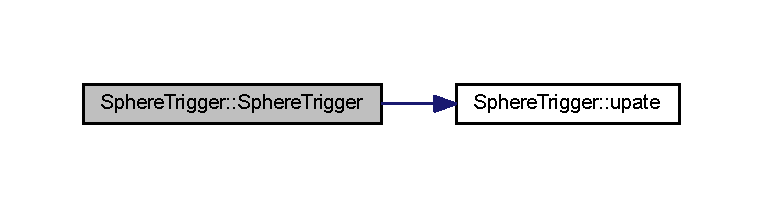
\includegraphics[width=350pt]{class_sphere_trigger_a4eddf434bac94055d32b0c5e37b24e0a_cgraph}
\end{center}
\end{figure}


\index{Sphere\+Trigger@{Sphere\+Trigger}!Sphere\+Trigger@{Sphere\+Trigger}}
\index{Sphere\+Trigger@{Sphere\+Trigger}!Sphere\+Trigger@{Sphere\+Trigger}}
\subsubsection[{\texorpdfstring{Sphere\+Trigger(const sf\+::\+Vector2f \&position, float f\+Radius)}{SphereTrigger(const sf::Vector2f &position, float fRadius)}}]{\setlength{\rightskip}{0pt plus 5cm}Sphere\+Trigger\+::\+Sphere\+Trigger (
\begin{DoxyParamCaption}
\item[{const sf\+::\+Vector2f \&}]{position, }
\item[{float}]{f\+Radius}
\end{DoxyParamCaption}
)}\hypertarget{class_sphere_trigger_ac7dfa0626d77354df9e99dcfc23023ec}{}\label{class_sphere_trigger_ac7dfa0626d77354df9e99dcfc23023ec}
Constructor. 
\begin{DoxyParams}{Parameters}
{\em position} & = Position of the circle. \\
\hline
{\em f\+Radius} & = Radius of the circle. \\
\hline
\end{DoxyParams}


\subsection{Member Function Documentation}
\index{Sphere\+Trigger@{Sphere\+Trigger}!upate@{upate}}
\index{upate@{upate}!Sphere\+Trigger@{Sphere\+Trigger}}
\subsubsection[{\texorpdfstring{upate(sf\+::\+Vector2f position)}{upate(sf::Vector2f position)}}]{\setlength{\rightskip}{0pt plus 5cm}void Sphere\+Trigger\+::upate (
\begin{DoxyParamCaption}
\item[{sf\+::\+Vector2f}]{position}
\end{DoxyParamCaption}
)}\hypertarget{class_sphere_trigger_af87f09551c86121cec4c9b0210de6166}{}\label{class_sphere_trigger_af87f09551c86121cec4c9b0210de6166}
Sphere update. 
\begin{DoxyParams}{Parameters}
{\em position} & = Position that needs updating. \\
\hline
\end{DoxyParams}


\subsection{Member Data Documentation}
\index{Sphere\+Trigger@{Sphere\+Trigger}!b\+Collision@{b\+Collision}}
\index{b\+Collision@{b\+Collision}!Sphere\+Trigger@{Sphere\+Trigger}}
\subsubsection[{\texorpdfstring{b\+Collision}{bCollision}}]{\setlength{\rightskip}{0pt plus 5cm}bool Sphere\+Trigger\+::b\+Collision\hspace{0.3cm}{\ttfamily [private]}}\hypertarget{class_sphere_trigger_aa2bbb652a3072e2041c75c01705486b9}{}\label{class_sphere_trigger_aa2bbb652a3072e2041c75c01705486b9}


The documentation for this class was generated from the following file\+:\begin{DoxyCompactItemize}
\item 
include/\hyperlink{sphere_trigger_8h}{sphere\+Trigger.\+h}\end{DoxyCompactItemize}

\hypertarget{class_static_car}{}\section{Static\+Car Class Reference}
\label{class_static_car}\index{Static\+Car@{Static\+Car}}


This class is used to create immovable cars.  




{\ttfamily \#include $<$static\+Car.\+h$>$}



Inheritance diagram for Static\+Car\+:\nopagebreak
\begin{figure}[H]
\begin{center}
\leavevmode
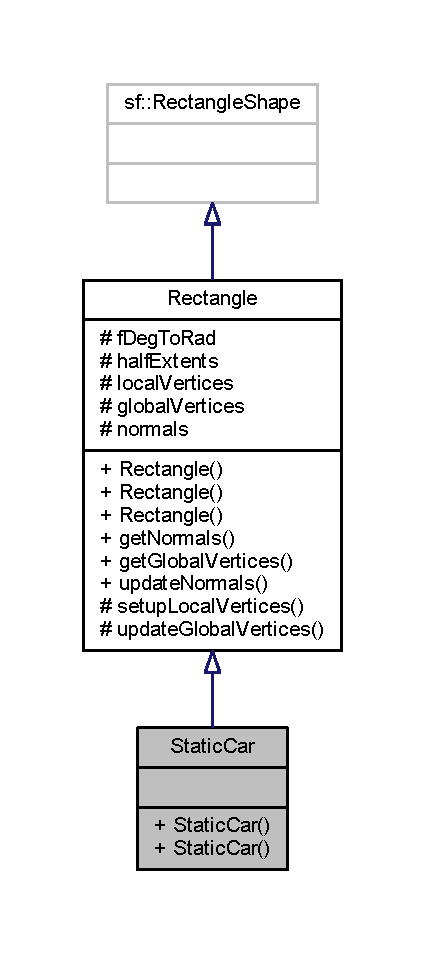
\includegraphics[width=204pt]{class_static_car__inherit__graph}
\end{center}
\end{figure}


Collaboration diagram for Static\+Car\+:\nopagebreak
\begin{figure}[H]
\begin{center}
\leavevmode
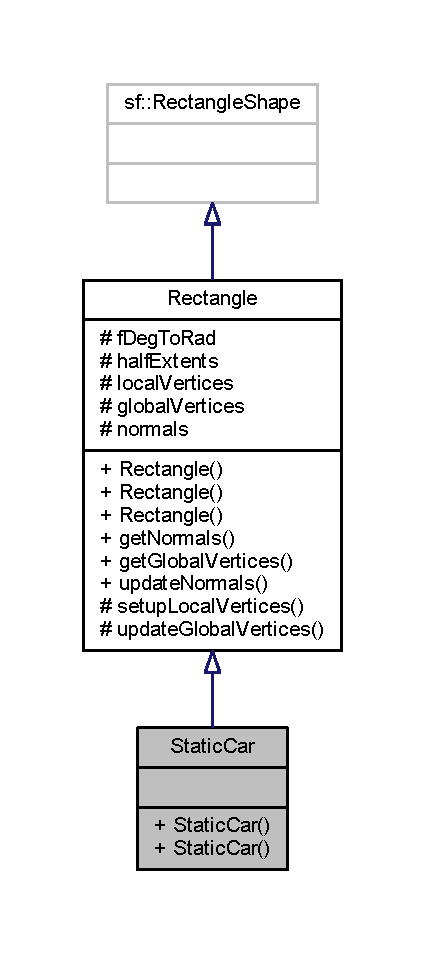
\includegraphics[width=204pt]{class_static_car__coll__graph}
\end{center}
\end{figure}
\subsection*{Public Member Functions}
\begin{DoxyCompactItemize}
\item 
\hyperlink{class_static_car_acb4b30c5dcb71e2aa2c48b0da9e4537b}{Static\+Car} ()
\item 
\hyperlink{class_static_car_a0242985cc1279fea1f6812bc61c30ca1}{Static\+Car} (const sf\+::\+Vector2f \&position, const sf\+::\+Vector2f \&dimensions, const sf\+::\+Texture \&texture, const float f\+Angle)
\end{DoxyCompactItemize}
\subsection*{Additional Inherited Members}


\subsection{Detailed Description}
This class is used to create immovable cars. 

\subsection{Constructor \& Destructor Documentation}
\index{Static\+Car@{Static\+Car}!Static\+Car@{Static\+Car}}
\index{Static\+Car@{Static\+Car}!Static\+Car@{Static\+Car}}
\subsubsection[{\texorpdfstring{Static\+Car()}{StaticCar()}}]{\setlength{\rightskip}{0pt plus 5cm}Static\+Car\+::\+Static\+Car (
\begin{DoxyParamCaption}
{}
\end{DoxyParamCaption}
)\hspace{0.3cm}{\ttfamily [inline]}}\hypertarget{class_static_car_acb4b30c5dcb71e2aa2c48b0da9e4537b}{}\label{class_static_car_acb4b30c5dcb71e2aa2c48b0da9e4537b}
Initializer. \index{Static\+Car@{Static\+Car}!Static\+Car@{Static\+Car}}
\index{Static\+Car@{Static\+Car}!Static\+Car@{Static\+Car}}
\subsubsection[{\texorpdfstring{Static\+Car(const sf\+::\+Vector2f \&position, const sf\+::\+Vector2f \&dimensions, const sf\+::\+Texture \&texture, const float f\+Angle)}{StaticCar(const sf::Vector2f &position, const sf::Vector2f &dimensions, const sf::Texture &texture, const float fAngle)}}]{\setlength{\rightskip}{0pt plus 5cm}Static\+Car\+::\+Static\+Car (
\begin{DoxyParamCaption}
\item[{const sf\+::\+Vector2f \&}]{position, }
\item[{const sf\+::\+Vector2f \&}]{dimensions, }
\item[{const sf\+::\+Texture \&}]{texture, }
\item[{const float}]{f\+Angle}
\end{DoxyParamCaption}
)}\hypertarget{class_static_car_a0242985cc1279fea1f6812bc61c30ca1}{}\label{class_static_car_a0242985cc1279fea1f6812bc61c30ca1}
Constructor. 
\begin{DoxyParams}{Parameters}
{\em position} & = Position of the rectangle. \\
\hline
{\em dimensions} & = Size of the rectangle. \\
\hline
{\em texture} & = Texture to load. \\
\hline
{\em f\+Angle} & = An orientation of the car \\
\hline
\end{DoxyParams}


The documentation for this class was generated from the following file\+:\begin{DoxyCompactItemize}
\item 
include/\hyperlink{static_car_8h}{static\+Car.\+h}\end{DoxyCompactItemize}

\hypertarget{class_texture_loader}{}\section{Texture\+Loader Class Reference}
\label{class_texture_loader}\index{Texture\+Loader@{Texture\+Loader}}


This class is used to manage textures.  




{\ttfamily \#include $<$texture\+Loader.\+h$>$}



Collaboration diagram for Texture\+Loader\+:\nopagebreak
\begin{figure}[H]
\begin{center}
\leavevmode
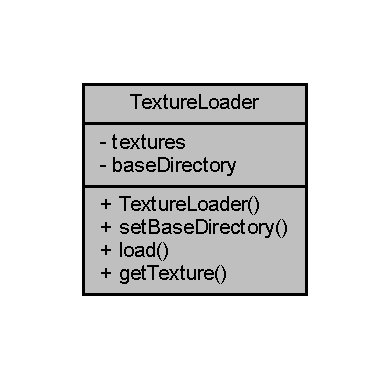
\includegraphics[width=187pt]{class_texture_loader__coll__graph}
\end{center}
\end{figure}
\subsection*{Public Member Functions}
\begin{DoxyCompactItemize}
\item 
\hyperlink{class_texture_loader_aafa6ca3bdbee3874a73aafae39d5c804}{Texture\+Loader} ()
\item 
void \hyperlink{class_texture_loader_a08f49a4b5cd9e0d5f84064de749b3eaf}{set\+Base\+Directory} (std\+::string dir)
\item 
void \hyperlink{class_texture_loader_a44ce52ccffb88baa49ba8128cc792ffc}{load} (std\+::vector$<$ std\+::string $>$ file\+Names)
\item 
sf\+::\+Texture \& \hyperlink{class_texture_loader_abfcc36c51b8d6a493040e01ed84f6bfc}{get\+Texture} (int f\+Index)
\end{DoxyCompactItemize}
\subsection*{Private Attributes}
\begin{DoxyCompactItemize}
\item 
std\+::vector$<$ sf\+::\+Texture $>$ \hyperlink{class_texture_loader_ad4e7dba3bb89484d7c92b702423cfc77}{textures}
\item 
std\+::string \hyperlink{class_texture_loader_acd647e9e5e5ca9b1ba8b3e6ef0aa9d84}{base\+Directory}
\end{DoxyCompactItemize}


\subsection{Detailed Description}
This class is used to manage textures. 

\subsection{Constructor \& Destructor Documentation}
\index{Texture\+Loader@{Texture\+Loader}!Texture\+Loader@{Texture\+Loader}}
\index{Texture\+Loader@{Texture\+Loader}!Texture\+Loader@{Texture\+Loader}}
\subsubsection[{\texorpdfstring{Texture\+Loader()}{TextureLoader()}}]{\setlength{\rightskip}{0pt plus 5cm}Texture\+Loader\+::\+Texture\+Loader (
\begin{DoxyParamCaption}
{}
\end{DoxyParamCaption}
)}\hypertarget{class_texture_loader_aafa6ca3bdbee3874a73aafae39d5c804}{}\label{class_texture_loader_aafa6ca3bdbee3874a73aafae39d5c804}
Initializer. 

\subsection{Member Function Documentation}
\index{Texture\+Loader@{Texture\+Loader}!get\+Texture@{get\+Texture}}
\index{get\+Texture@{get\+Texture}!Texture\+Loader@{Texture\+Loader}}
\subsubsection[{\texorpdfstring{get\+Texture(int f\+Index)}{getTexture(int fIndex)}}]{\setlength{\rightskip}{0pt plus 5cm}sf\+::\+Texture\& Texture\+Loader\+::get\+Texture (
\begin{DoxyParamCaption}
\item[{int}]{f\+Index}
\end{DoxyParamCaption}
)}\hypertarget{class_texture_loader_abfcc36c51b8d6a493040e01ed84f6bfc}{}\label{class_texture_loader_abfcc36c51b8d6a493040e01ed84f6bfc}
Returns texture with said index. 
\begin{DoxyParams}{Parameters}
{\em f\+Index} & = Index of the texture. \\
\hline
\end{DoxyParams}
\begin{DoxyReturn}{Returns}
$\ast$it = Retruns pointer to the texture with matching index. 
\end{DoxyReturn}
\index{Texture\+Loader@{Texture\+Loader}!load@{load}}
\index{load@{load}!Texture\+Loader@{Texture\+Loader}}
\subsubsection[{\texorpdfstring{load(std\+::vector$<$ std\+::string $>$ file\+Names)}{load(std::vector< std::string > fileNames)}}]{\setlength{\rightskip}{0pt plus 5cm}void Texture\+Loader\+::load (
\begin{DoxyParamCaption}
\item[{std\+::vector$<$ std\+::string $>$}]{file\+Names}
\end{DoxyParamCaption}
)}\hypertarget{class_texture_loader_a44ce52ccffb88baa49ba8128cc792ffc}{}\label{class_texture_loader_a44ce52ccffb88baa49ba8128cc792ffc}
Loads textures based on the string input. 
\begin{DoxyParams}{Parameters}
{\em file\+Names} & = String vector with file names. \\
\hline
\end{DoxyParams}
\index{Texture\+Loader@{Texture\+Loader}!set\+Base\+Directory@{set\+Base\+Directory}}
\index{set\+Base\+Directory@{set\+Base\+Directory}!Texture\+Loader@{Texture\+Loader}}
\subsubsection[{\texorpdfstring{set\+Base\+Directory(std\+::string dir)}{setBaseDirectory(std::string dir)}}]{\setlength{\rightskip}{0pt plus 5cm}void Texture\+Loader\+::set\+Base\+Directory (
\begin{DoxyParamCaption}
\item[{std\+::string}]{dir}
\end{DoxyParamCaption}
)}\hypertarget{class_texture_loader_a08f49a4b5cd9e0d5f84064de749b3eaf}{}\label{class_texture_loader_a08f49a4b5cd9e0d5f84064de749b3eaf}
Sets our base directory. 
\begin{DoxyParams}{Parameters}
{\em dir} & = Our base directory. \\
\hline
\end{DoxyParams}


\subsection{Member Data Documentation}
\index{Texture\+Loader@{Texture\+Loader}!base\+Directory@{base\+Directory}}
\index{base\+Directory@{base\+Directory}!Texture\+Loader@{Texture\+Loader}}
\subsubsection[{\texorpdfstring{base\+Directory}{baseDirectory}}]{\setlength{\rightskip}{0pt plus 5cm}std\+::string Texture\+Loader\+::base\+Directory\hspace{0.3cm}{\ttfamily [private]}}\hypertarget{class_texture_loader_acd647e9e5e5ca9b1ba8b3e6ef0aa9d84}{}\label{class_texture_loader_acd647e9e5e5ca9b1ba8b3e6ef0aa9d84}
Our base directory with textures. \index{Texture\+Loader@{Texture\+Loader}!textures@{textures}}
\index{textures@{textures}!Texture\+Loader@{Texture\+Loader}}
\subsubsection[{\texorpdfstring{textures}{textures}}]{\setlength{\rightskip}{0pt plus 5cm}std\+::vector$<$sf\+::\+Texture$>$ Texture\+Loader\+::textures\hspace{0.3cm}{\ttfamily [private]}}\hypertarget{class_texture_loader_ad4e7dba3bb89484d7c92b702423cfc77}{}\label{class_texture_loader_ad4e7dba3bb89484d7c92b702423cfc77}
Vector of textures. 

The documentation for this class was generated from the following file\+:\begin{DoxyCompactItemize}
\item 
include/\hyperlink{texture_loader_8h}{texture\+Loader.\+h}\end{DoxyCompactItemize}

\hypertarget{class_tire}{}\section{Tire Class Reference}
\label{class_tire}\index{Tire@{Tire}}


This class is used to construct a tire.  




{\ttfamily \#include $<$tire.\+h$>$}



Inheritance diagram for Tire\+:\nopagebreak
\begin{figure}[H]
\begin{center}
\leavevmode
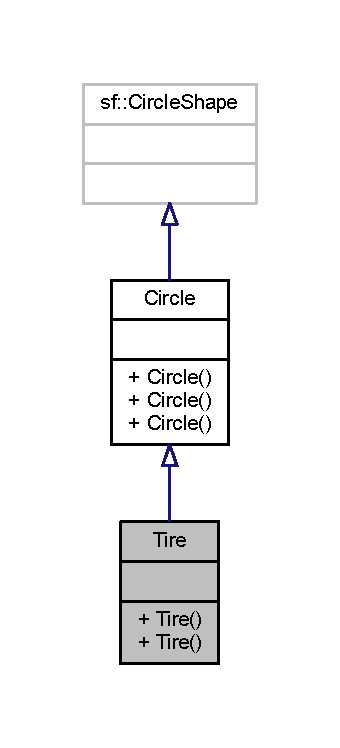
\includegraphics[width=163pt]{class_tire__inherit__graph}
\end{center}
\end{figure}


Collaboration diagram for Tire\+:\nopagebreak
\begin{figure}[H]
\begin{center}
\leavevmode
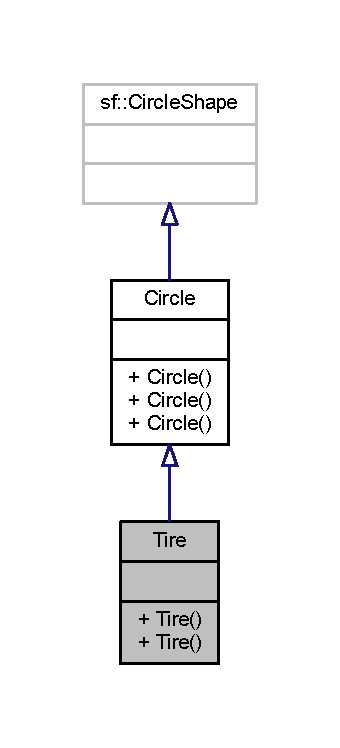
\includegraphics[width=163pt]{class_tire__coll__graph}
\end{center}
\end{figure}
\subsection*{Public Member Functions}
\begin{DoxyCompactItemize}
\item 
\hyperlink{class_tire_a35b9abbd0ad6e265c1d0c34a9f825abb}{Tire} ()
\item 
\hyperlink{class_tire_a68d4d8c5a3e918150796549e81fe173b}{Tire} (sf\+::\+Vector2f \&position, float f\+Radius, sf\+::\+Texture \&texture)
\end{DoxyCompactItemize}


\subsection{Detailed Description}
This class is used to construct a tire. 

\subsection{Constructor \& Destructor Documentation}
\index{Tire@{Tire}!Tire@{Tire}}
\index{Tire@{Tire}!Tire@{Tire}}
\subsubsection[{\texorpdfstring{Tire()}{Tire()}}]{\setlength{\rightskip}{0pt plus 5cm}Tire\+::\+Tire (
\begin{DoxyParamCaption}
{}
\end{DoxyParamCaption}
)\hspace{0.3cm}{\ttfamily [inline]}}\hypertarget{class_tire_a35b9abbd0ad6e265c1d0c34a9f825abb}{}\label{class_tire_a35b9abbd0ad6e265c1d0c34a9f825abb}
Initializer. \index{Tire@{Tire}!Tire@{Tire}}
\index{Tire@{Tire}!Tire@{Tire}}
\subsubsection[{\texorpdfstring{Tire(sf\+::\+Vector2f \&position, float f\+Radius, sf\+::\+Texture \&texture)}{Tire(sf::Vector2f &position, float fRadius, sf::Texture &texture)}}]{\setlength{\rightskip}{0pt plus 5cm}Tire\+::\+Tire (
\begin{DoxyParamCaption}
\item[{sf\+::\+Vector2f \&}]{position, }
\item[{float}]{f\+Radius, }
\item[{sf\+::\+Texture \&}]{texture}
\end{DoxyParamCaption}
)}\hypertarget{class_tire_a68d4d8c5a3e918150796549e81fe173b}{}\label{class_tire_a68d4d8c5a3e918150796549e81fe173b}
Constructor. 
\begin{DoxyParams}{Parameters}
{\em position} & = Position of the tire. \\
\hline
{\em f\+Radius} & = Radius of the tire. \\
\hline
{\em texture} & = Texture to load. \\
\hline
\end{DoxyParams}


The documentation for this class was generated from the following file\+:\begin{DoxyCompactItemize}
\item 
include/\hyperlink{tire_8h}{tire.\+h}\end{DoxyCompactItemize}

\hypertarget{class_vector_maths}{}\section{Vector\+Maths Class Reference}
\label{class_vector_maths}\index{Vector\+Maths@{Vector\+Maths}}


This class is used to do simple vector calculations.  




{\ttfamily \#include $<$vector\+Maths.\+h$>$}



Collaboration diagram for Vector\+Maths\+:\nopagebreak
\begin{figure}[H]
\begin{center}
\leavevmode
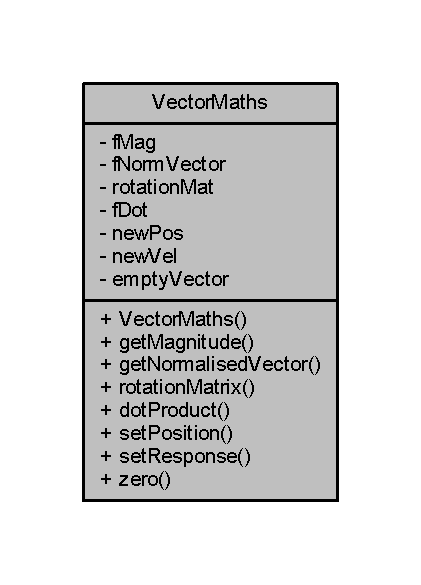
\includegraphics[width=202pt]{class_vector_maths__coll__graph}
\end{center}
\end{figure}
\subsection*{Public Member Functions}
\begin{DoxyCompactItemize}
\item 
\hyperlink{class_vector_maths_af14f2937b1a287972ae741082c63e6e2}{Vector\+Maths} ()
\item 
float \hyperlink{class_vector_maths_ac32142cb1d6a374e3808842c42aad1bf}{get\+Magnitude} (sf\+::\+Vector2f some\+Vector)
\item 
sf\+::\+Vector2f \hyperlink{class_vector_maths_a2958671bb1fabcaa012fa7a96764f0c3}{get\+Normalised\+Vector} (sf\+::\+Vector2f some\+Vector)
\item 
sf\+::\+Vector2f \hyperlink{class_vector_maths_abf04ac83d6af1aff50447fc3e9a510da}{rotation\+Matrix} (sf\+::\+Vector2f some\+Vector, float f\+Angle)
\item 
float \hyperlink{class_vector_maths_a53b54c300f657d8eb0859b9456c4fd40}{dot\+Product} (sf\+::\+Vector2f first, sf\+::\+Vector2f second)
\item 
sf\+::\+Vector2f \hyperlink{class_vector_maths_af669b52c8b757560e8c7d1af263acbf4}{set\+Position} (sf\+::\+Vector2f position, sf\+::\+Vector2f collision\+Normal, float f\+Overlap)
\item 
sf\+::\+Vector2f \hyperlink{class_vector_maths_a3e5d8270e32fb2985657e05ff20a3e57}{set\+Response} (sf\+::\+Vector2f velocity, sf\+::\+Vector2f collision\+Normal, float f\+Restitution)
\item 
sf\+::\+Vector2f \hyperlink{class_vector_maths_a100430d2798e19d383c68cae5f3a35ec}{zero} ()
\end{DoxyCompactItemize}
\subsection*{Private Attributes}
\begin{DoxyCompactItemize}
\item 
float \hyperlink{class_vector_maths_a500410fcab46699e06a8b7dadf56771d}{f\+Mag}
\item 
sf\+::\+Vector2f \hyperlink{class_vector_maths_a28a7d7f8fc60f6c0b35e7896a5ec48d5}{f\+Norm\+Vector}
\item 
sf\+::\+Vector2f \hyperlink{class_vector_maths_ae07f69982afee9ac9532c70e4bcde1d3}{rotation\+Mat}
\item 
float \hyperlink{class_vector_maths_a1f152ea5bd11ef07643bea0de8d2a75c}{f\+Dot}
\item 
sf\+::\+Vector2f \hyperlink{class_vector_maths_abc596252a016b278d89649aa84a788f6}{new\+Pos}
\item 
sf\+::\+Vector2f \hyperlink{class_vector_maths_a00513ada0f74184f044eb6fc35aa4a85}{new\+Vel}
\item 
sf\+::\+Vector2f \hyperlink{class_vector_maths_a701ff35f136062ae5e43b76e5f39c3e3}{empty\+Vector}
\end{DoxyCompactItemize}


\subsection{Detailed Description}
This class is used to do simple vector calculations. 

\subsection{Constructor \& Destructor Documentation}
\index{Vector\+Maths@{Vector\+Maths}!Vector\+Maths@{Vector\+Maths}}
\index{Vector\+Maths@{Vector\+Maths}!Vector\+Maths@{Vector\+Maths}}
\subsubsection[{\texorpdfstring{Vector\+Maths()}{VectorMaths()}}]{\setlength{\rightskip}{0pt plus 5cm}Vector\+Maths\+::\+Vector\+Maths (
\begin{DoxyParamCaption}
{}
\end{DoxyParamCaption}
)\hspace{0.3cm}{\ttfamily [inline]}}\hypertarget{class_vector_maths_af14f2937b1a287972ae741082c63e6e2}{}\label{class_vector_maths_af14f2937b1a287972ae741082c63e6e2}
Initializer. 

Here is the call graph for this function\+:\nopagebreak
\begin{figure}[H]
\begin{center}
\leavevmode
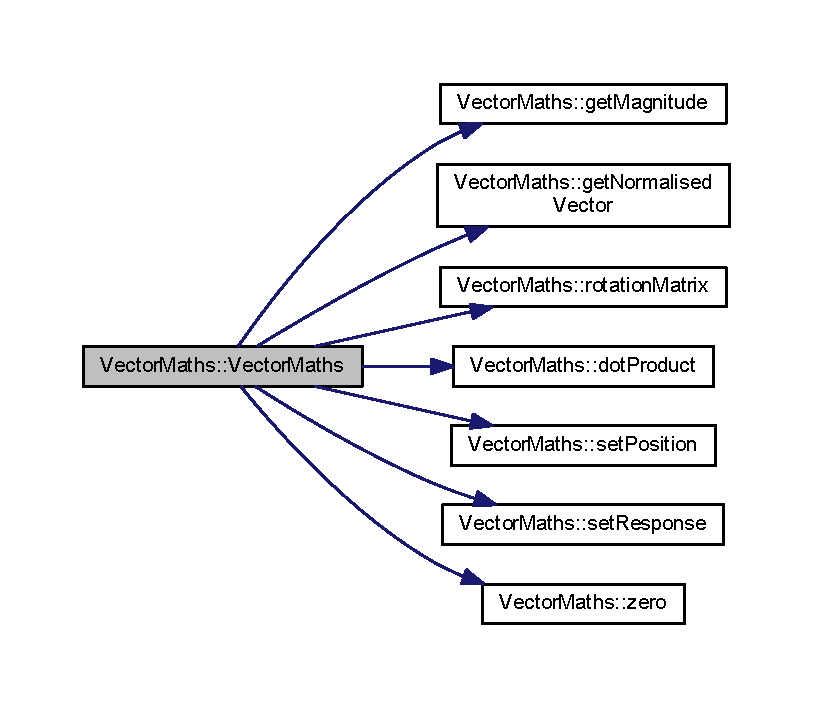
\includegraphics[width=350pt]{class_vector_maths_af14f2937b1a287972ae741082c63e6e2_cgraph}
\end{center}
\end{figure}




\subsection{Member Function Documentation}
\index{Vector\+Maths@{Vector\+Maths}!dot\+Product@{dot\+Product}}
\index{dot\+Product@{dot\+Product}!Vector\+Maths@{Vector\+Maths}}
\subsubsection[{\texorpdfstring{dot\+Product(sf\+::\+Vector2f first, sf\+::\+Vector2f second)}{dotProduct(sf::Vector2f first, sf::Vector2f second)}}]{\setlength{\rightskip}{0pt plus 5cm}float Vector\+Maths\+::dot\+Product (
\begin{DoxyParamCaption}
\item[{sf\+::\+Vector2f}]{first, }
\item[{sf\+::\+Vector2f}]{second}
\end{DoxyParamCaption}
)}\hypertarget{class_vector_maths_a53b54c300f657d8eb0859b9456c4fd40}{}\label{class_vector_maths_a53b54c300f657d8eb0859b9456c4fd40}
Calculates a dot product. 
\begin{DoxyParams}{Parameters}
{\em first} & = A first vector. \\
\hline
{\em second} & = A second vector. \\
\hline
\end{DoxyParams}
\begin{DoxyReturn}{Returns}
f\+Dot = Returns a dot product of two vectors. 
\end{DoxyReturn}
\index{Vector\+Maths@{Vector\+Maths}!get\+Magnitude@{get\+Magnitude}}
\index{get\+Magnitude@{get\+Magnitude}!Vector\+Maths@{Vector\+Maths}}
\subsubsection[{\texorpdfstring{get\+Magnitude(sf\+::\+Vector2f some\+Vector)}{getMagnitude(sf::Vector2f someVector)}}]{\setlength{\rightskip}{0pt plus 5cm}float Vector\+Maths\+::get\+Magnitude (
\begin{DoxyParamCaption}
\item[{sf\+::\+Vector2f}]{some\+Vector}
\end{DoxyParamCaption}
)}\hypertarget{class_vector_maths_ac32142cb1d6a374e3808842c42aad1bf}{}\label{class_vector_maths_ac32142cb1d6a374e3808842c42aad1bf}
Calculates a magnitude of a vector. 
\begin{DoxyParams}{Parameters}
{\em some\+Vector} & = We will calculate magnitude of that vector. \\
\hline
\end{DoxyParams}
\begin{DoxyReturn}{Returns}
f\+Mag = Magnitude of a vector. 
\end{DoxyReturn}
\index{Vector\+Maths@{Vector\+Maths}!get\+Normalised\+Vector@{get\+Normalised\+Vector}}
\index{get\+Normalised\+Vector@{get\+Normalised\+Vector}!Vector\+Maths@{Vector\+Maths}}
\subsubsection[{\texorpdfstring{get\+Normalised\+Vector(sf\+::\+Vector2f some\+Vector)}{getNormalisedVector(sf::Vector2f someVector)}}]{\setlength{\rightskip}{0pt plus 5cm}sf\+::\+Vector2f Vector\+Maths\+::get\+Normalised\+Vector (
\begin{DoxyParamCaption}
\item[{sf\+::\+Vector2f}]{some\+Vector}
\end{DoxyParamCaption}
)}\hypertarget{class_vector_maths_a2958671bb1fabcaa012fa7a96764f0c3}{}\label{class_vector_maths_a2958671bb1fabcaa012fa7a96764f0c3}
Calculates a normalised vector. 
\begin{DoxyParams}{Parameters}
{\em some\+Vector} & = We will calculate unit vector of that vector. \\
\hline
\end{DoxyParams}
\begin{DoxyReturn}{Returns}
f\+Norm\+Vector = Returns a normalised vector. 
\end{DoxyReturn}
\index{Vector\+Maths@{Vector\+Maths}!rotation\+Matrix@{rotation\+Matrix}}
\index{rotation\+Matrix@{rotation\+Matrix}!Vector\+Maths@{Vector\+Maths}}
\subsubsection[{\texorpdfstring{rotation\+Matrix(sf\+::\+Vector2f some\+Vector, float f\+Angle)}{rotationMatrix(sf::Vector2f someVector, float fAngle)}}]{\setlength{\rightskip}{0pt plus 5cm}sf\+::\+Vector2f Vector\+Maths\+::rotation\+Matrix (
\begin{DoxyParamCaption}
\item[{sf\+::\+Vector2f}]{some\+Vector, }
\item[{float}]{f\+Angle}
\end{DoxyParamCaption}
)}\hypertarget{class_vector_maths_abf04ac83d6af1aff50447fc3e9a510da}{}\label{class_vector_maths_abf04ac83d6af1aff50447fc3e9a510da}
Calculates a rotation matrix. 
\begin{DoxyParams}{Parameters}
{\em some\+Vector} & = A vector to be used in rotation. \\
\hline
{\em f\+Angle} & = An angle at which we will rotate the vector. \\
\hline
\end{DoxyParams}
\begin{DoxyReturn}{Returns}
temp = Vector with applied matrix. 
\end{DoxyReturn}
\index{Vector\+Maths@{Vector\+Maths}!set\+Position@{set\+Position}}
\index{set\+Position@{set\+Position}!Vector\+Maths@{Vector\+Maths}}
\subsubsection[{\texorpdfstring{set\+Position(sf\+::\+Vector2f position, sf\+::\+Vector2f collision\+Normal, float f\+Overlap)}{setPosition(sf::Vector2f position, sf::Vector2f collisionNormal, float fOverlap)}}]{\setlength{\rightskip}{0pt plus 5cm}sf\+::\+Vector2f Vector\+Maths\+::set\+Position (
\begin{DoxyParamCaption}
\item[{sf\+::\+Vector2f}]{position, }
\item[{sf\+::\+Vector2f}]{collision\+Normal, }
\item[{float}]{f\+Overlap}
\end{DoxyParamCaption}
)}\hypertarget{class_vector_maths_af669b52c8b757560e8c7d1af263acbf4}{}\label{class_vector_maths_af669b52c8b757560e8c7d1af263acbf4}
Reposition an object. 
\begin{DoxyParams}{Parameters}
{\em position} & = A position of the object we want apply new position to. \\
\hline
{\em collision\+Normal} & = A collision normal from the collision test. \\
\hline
{\em f\+Overlap} & = The smallest overlap from the collision test. \\
\hline
\end{DoxyParams}
\begin{DoxyReturn}{Returns}
new\+Pos = Returns new position with applied changes. 
\end{DoxyReturn}
\index{Vector\+Maths@{Vector\+Maths}!set\+Response@{set\+Response}}
\index{set\+Response@{set\+Response}!Vector\+Maths@{Vector\+Maths}}
\subsubsection[{\texorpdfstring{set\+Response(sf\+::\+Vector2f velocity, sf\+::\+Vector2f collision\+Normal, float f\+Restitution)}{setResponse(sf::Vector2f velocity, sf::Vector2f collisionNormal, float fRestitution)}}]{\setlength{\rightskip}{0pt plus 5cm}sf\+::\+Vector2f Vector\+Maths\+::set\+Response (
\begin{DoxyParamCaption}
\item[{sf\+::\+Vector2f}]{velocity, }
\item[{sf\+::\+Vector2f}]{collision\+Normal, }
\item[{float}]{f\+Restitution}
\end{DoxyParamCaption}
)}\hypertarget{class_vector_maths_a3e5d8270e32fb2985657e05ff20a3e57}{}\label{class_vector_maths_a3e5d8270e32fb2985657e05ff20a3e57}
\hyperlink{class_collision}{Collision} response. 
\begin{DoxyParams}{Parameters}
{\em velocity} & = A velocioty of the object we want apply response to. \\
\hline
{\em collision\+Normal} & = A collision normal from the collision test. \\
\hline
{\em f\+Restitution} & = Coeffcient of restitution. \\
\hline
\end{DoxyParams}
\begin{DoxyReturn}{Returns}
new\+Vel = Returns new velocity with applied response. 
\end{DoxyReturn}
\index{Vector\+Maths@{Vector\+Maths}!zero@{zero}}
\index{zero@{zero}!Vector\+Maths@{Vector\+Maths}}
\subsubsection[{\texorpdfstring{zero()}{zero()}}]{\setlength{\rightskip}{0pt plus 5cm}sf\+::\+Vector2f Vector\+Maths\+::zero (
\begin{DoxyParamCaption}
{}
\end{DoxyParamCaption}
)}\hypertarget{class_vector_maths_a100430d2798e19d383c68cae5f3a35ec}{}\label{class_vector_maths_a100430d2798e19d383c68cae5f3a35ec}
Vector2f (0.\+f, 0.\+f) . \begin{DoxyReturn}{Returns}
empty\+Vel = Returns an empty vector. 
\end{DoxyReturn}


\subsection{Member Data Documentation}
\index{Vector\+Maths@{Vector\+Maths}!empty\+Vector@{empty\+Vector}}
\index{empty\+Vector@{empty\+Vector}!Vector\+Maths@{Vector\+Maths}}
\subsubsection[{\texorpdfstring{empty\+Vector}{emptyVector}}]{\setlength{\rightskip}{0pt plus 5cm}sf\+::\+Vector2f Vector\+Maths\+::empty\+Vector\hspace{0.3cm}{\ttfamily [private]}}\hypertarget{class_vector_maths_a701ff35f136062ae5e43b76e5f39c3e3}{}\label{class_vector_maths_a701ff35f136062ae5e43b76e5f39c3e3}
An empty vector. \index{Vector\+Maths@{Vector\+Maths}!f\+Dot@{f\+Dot}}
\index{f\+Dot@{f\+Dot}!Vector\+Maths@{Vector\+Maths}}
\subsubsection[{\texorpdfstring{f\+Dot}{fDot}}]{\setlength{\rightskip}{0pt plus 5cm}float Vector\+Maths\+::f\+Dot\hspace{0.3cm}{\ttfamily [private]}}\hypertarget{class_vector_maths_a1f152ea5bd11ef07643bea0de8d2a75c}{}\label{class_vector_maths_a1f152ea5bd11ef07643bea0de8d2a75c}
Dot product. \index{Vector\+Maths@{Vector\+Maths}!f\+Mag@{f\+Mag}}
\index{f\+Mag@{f\+Mag}!Vector\+Maths@{Vector\+Maths}}
\subsubsection[{\texorpdfstring{f\+Mag}{fMag}}]{\setlength{\rightskip}{0pt plus 5cm}float Vector\+Maths\+::f\+Mag\hspace{0.3cm}{\ttfamily [private]}}\hypertarget{class_vector_maths_a500410fcab46699e06a8b7dadf56771d}{}\label{class_vector_maths_a500410fcab46699e06a8b7dadf56771d}
Magnitude. \index{Vector\+Maths@{Vector\+Maths}!f\+Norm\+Vector@{f\+Norm\+Vector}}
\index{f\+Norm\+Vector@{f\+Norm\+Vector}!Vector\+Maths@{Vector\+Maths}}
\subsubsection[{\texorpdfstring{f\+Norm\+Vector}{fNormVector}}]{\setlength{\rightskip}{0pt plus 5cm}sf\+::\+Vector2f Vector\+Maths\+::f\+Norm\+Vector\hspace{0.3cm}{\ttfamily [private]}}\hypertarget{class_vector_maths_a28a7d7f8fc60f6c0b35e7896a5ec48d5}{}\label{class_vector_maths_a28a7d7f8fc60f6c0b35e7896a5ec48d5}
Normalised vector. \index{Vector\+Maths@{Vector\+Maths}!new\+Pos@{new\+Pos}}
\index{new\+Pos@{new\+Pos}!Vector\+Maths@{Vector\+Maths}}
\subsubsection[{\texorpdfstring{new\+Pos}{newPos}}]{\setlength{\rightskip}{0pt plus 5cm}sf\+::\+Vector2f Vector\+Maths\+::new\+Pos\hspace{0.3cm}{\ttfamily [private]}}\hypertarget{class_vector_maths_abc596252a016b278d89649aa84a788f6}{}\label{class_vector_maths_abc596252a016b278d89649aa84a788f6}
New position. \index{Vector\+Maths@{Vector\+Maths}!new\+Vel@{new\+Vel}}
\index{new\+Vel@{new\+Vel}!Vector\+Maths@{Vector\+Maths}}
\subsubsection[{\texorpdfstring{new\+Vel}{newVel}}]{\setlength{\rightskip}{0pt plus 5cm}sf\+::\+Vector2f Vector\+Maths\+::new\+Vel\hspace{0.3cm}{\ttfamily [private]}}\hypertarget{class_vector_maths_a00513ada0f74184f044eb6fc35aa4a85}{}\label{class_vector_maths_a00513ada0f74184f044eb6fc35aa4a85}
New velocity. \index{Vector\+Maths@{Vector\+Maths}!rotation\+Mat@{rotation\+Mat}}
\index{rotation\+Mat@{rotation\+Mat}!Vector\+Maths@{Vector\+Maths}}
\subsubsection[{\texorpdfstring{rotation\+Mat}{rotationMat}}]{\setlength{\rightskip}{0pt plus 5cm}sf\+::\+Vector2f Vector\+Maths\+::rotation\+Mat\hspace{0.3cm}{\ttfamily [private]}}\hypertarget{class_vector_maths_ae07f69982afee9ac9532c70e4bcde1d3}{}\label{class_vector_maths_ae07f69982afee9ac9532c70e4bcde1d3}
Rotation matrix. 

The documentation for this class was generated from the following file\+:\begin{DoxyCompactItemize}
\item 
include/\hyperlink{vector_maths_8h}{vector\+Maths.\+h}\end{DoxyCompactItemize}

\hypertarget{class_view}{}\section{View Class Reference}
\label{class_view}\index{View@{View}}


This class is used to manage a scene.  




{\ttfamily \#include $<$view.\+h$>$}



Inheritance diagram for View\+:\nopagebreak
\begin{figure}[H]
\begin{center}
\leavevmode
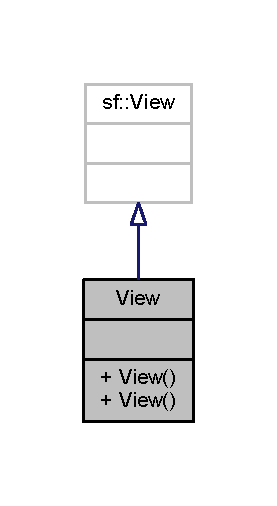
\includegraphics[width=133pt]{class_view__inherit__graph}
\end{center}
\end{figure}


Collaboration diagram for View\+:\nopagebreak
\begin{figure}[H]
\begin{center}
\leavevmode
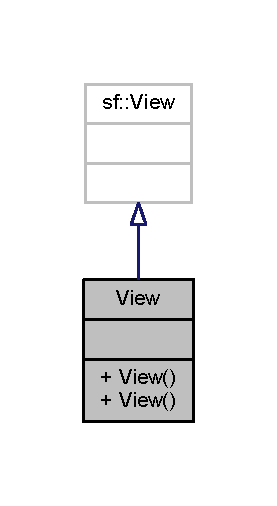
\includegraphics[width=133pt]{class_view__coll__graph}
\end{center}
\end{figure}
\subsection*{Public Member Functions}
\begin{DoxyCompactItemize}
\item 
\hyperlink{class_view_a44ad60a768422d3fa8fbd7576950080a}{View} ()
\item 
\hyperlink{class_view_a1d83f87d9cfff8c62730ac905a05e77a}{View} (const sf\+::\+Vector2f \&dimensions, const sf\+::\+Vector2f \&centre, const float \&f\+Zoom)
\end{DoxyCompactItemize}


\subsection{Detailed Description}
This class is used to manage a scene. 

\subsection{Constructor \& Destructor Documentation}
\index{View@{View}!View@{View}}
\index{View@{View}!View@{View}}
\subsubsection[{\texorpdfstring{View()}{View()}}]{\setlength{\rightskip}{0pt plus 5cm}View\+::\+View (
\begin{DoxyParamCaption}
{}
\end{DoxyParamCaption}
)\hspace{0.3cm}{\ttfamily [inline]}}\hypertarget{class_view_a44ad60a768422d3fa8fbd7576950080a}{}\label{class_view_a44ad60a768422d3fa8fbd7576950080a}
Initializer. \index{View@{View}!View@{View}}
\index{View@{View}!View@{View}}
\subsubsection[{\texorpdfstring{View(const sf\+::\+Vector2f \&dimensions, const sf\+::\+Vector2f \&centre, const float \&f\+Zoom)}{View(const sf::Vector2f &dimensions, const sf::Vector2f &centre, const float &fZoom)}}]{\setlength{\rightskip}{0pt plus 5cm}View\+::\+View (
\begin{DoxyParamCaption}
\item[{const sf\+::\+Vector2f \&}]{dimensions, }
\item[{const sf\+::\+Vector2f \&}]{centre, }
\item[{const float \&}]{f\+Zoom}
\end{DoxyParamCaption}
)}\hypertarget{class_view_a1d83f87d9cfff8c62730ac905a05e77a}{}\label{class_view_a1d83f87d9cfff8c62730ac905a05e77a}
Constructor. 
\begin{DoxyParams}{Parameters}
{\em dimensions} & = Size of the view. \\
\hline
{\em centre} & = Centre of the view. \\
\hline
{\em f\+Zoom} & = Zoom in or out from the centre of the view. \\
\hline
\end{DoxyParams}


The documentation for this class was generated from the following file\+:\begin{DoxyCompactItemize}
\item 
include/\hyperlink{view_8h}{view.\+h}\end{DoxyCompactItemize}

\hypertarget{class_wall}{}\section{Wall Class Reference}
\label{class_wall}\index{Wall@{Wall}}


This class is used to construct a wall.  




{\ttfamily \#include $<$wall.\+h$>$}



Inheritance diagram for Wall\+:\nopagebreak
\begin{figure}[H]
\begin{center}
\leavevmode
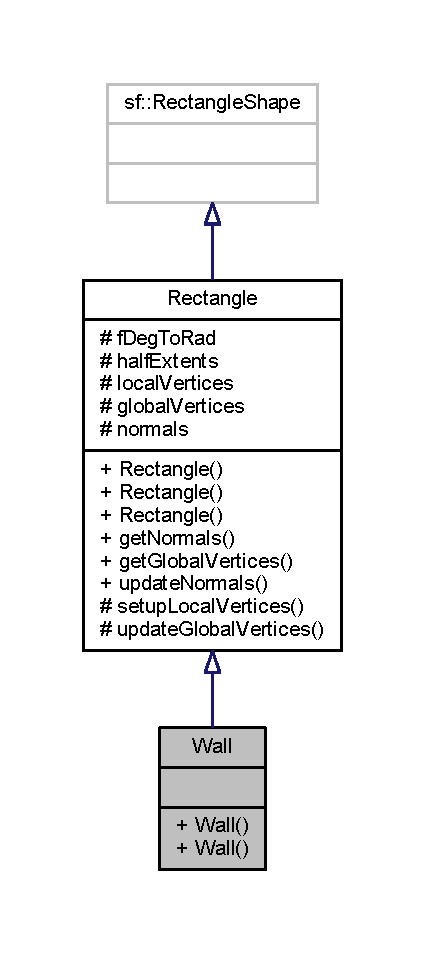
\includegraphics[width=204pt]{class_wall__inherit__graph}
\end{center}
\end{figure}


Collaboration diagram for Wall\+:\nopagebreak
\begin{figure}[H]
\begin{center}
\leavevmode
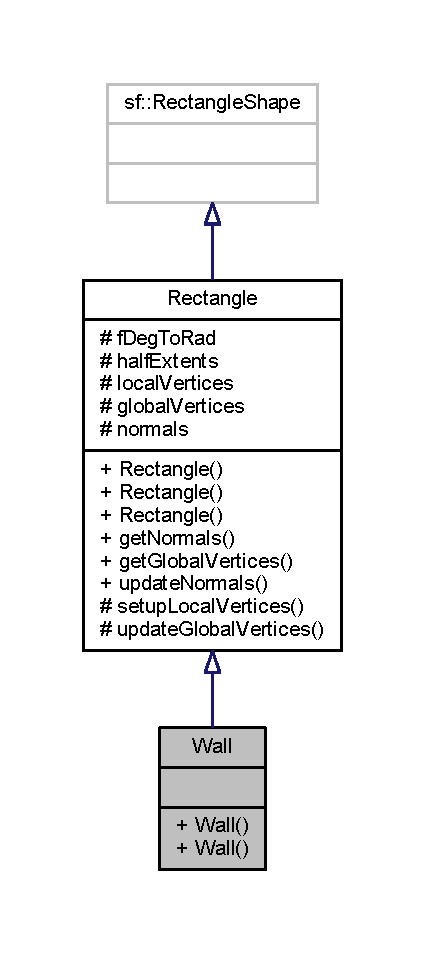
\includegraphics[width=204pt]{class_wall__coll__graph}
\end{center}
\end{figure}
\subsection*{Public Member Functions}
\begin{DoxyCompactItemize}
\item 
\hyperlink{class_wall_a12dc41bc7bc045c55ec1034a43e52043}{Wall} ()
\item 
\hyperlink{class_wall_ac17ed352213a1f0a3918c736e2840e82}{Wall} (sf\+::\+Vector2f \&position, sf\+::\+Vector2f \&dimensions, sf\+::\+Texture \&texture)
\end{DoxyCompactItemize}
\subsection*{Additional Inherited Members}


\subsection{Detailed Description}
This class is used to construct a wall. 

\subsection{Constructor \& Destructor Documentation}
\index{Wall@{Wall}!Wall@{Wall}}
\index{Wall@{Wall}!Wall@{Wall}}
\subsubsection[{\texorpdfstring{Wall()}{Wall()}}]{\setlength{\rightskip}{0pt plus 5cm}Wall\+::\+Wall (
\begin{DoxyParamCaption}
{}
\end{DoxyParamCaption}
)\hspace{0.3cm}{\ttfamily [inline]}}\hypertarget{class_wall_a12dc41bc7bc045c55ec1034a43e52043}{}\label{class_wall_a12dc41bc7bc045c55ec1034a43e52043}
Initializer. \index{Wall@{Wall}!Wall@{Wall}}
\index{Wall@{Wall}!Wall@{Wall}}
\subsubsection[{\texorpdfstring{Wall(sf\+::\+Vector2f \&position, sf\+::\+Vector2f \&dimensions, sf\+::\+Texture \&texture)}{Wall(sf::Vector2f &position, sf::Vector2f &dimensions, sf::Texture &texture)}}]{\setlength{\rightskip}{0pt plus 5cm}Wall\+::\+Wall (
\begin{DoxyParamCaption}
\item[{sf\+::\+Vector2f \&}]{position, }
\item[{sf\+::\+Vector2f \&}]{dimensions, }
\item[{sf\+::\+Texture \&}]{texture}
\end{DoxyParamCaption}
)}\hypertarget{class_wall_ac17ed352213a1f0a3918c736e2840e82}{}\label{class_wall_ac17ed352213a1f0a3918c736e2840e82}
Constructor. 
\begin{DoxyParams}{Parameters}
{\em position} & = Position of the wall. \\
\hline
{\em dimensions} & = Size of the wall. \\
\hline
{\em texture} & = Texture to load. \\
\hline
\end{DoxyParams}


The documentation for this class was generated from the following file\+:\begin{DoxyCompactItemize}
\item 
include/\hyperlink{wall_8h}{wall.\+h}\end{DoxyCompactItemize}

\chapter{File Documentation}
\hypertarget{audio_loader_8h}{}\section{include/audio\+Loader.h File Reference}
\label{audio_loader_8h}\index{include/audio\+Loader.\+h@{include/audio\+Loader.\+h}}
{\ttfamily \#include $<$S\+F\+M\+L\textbackslash{}\+Audio.\+hpp$>$}\\*
{\ttfamily \#include $<$array$>$}\\*
Include dependency graph for audio\+Loader.\+h\+:\nopagebreak
\begin{figure}[H]
\begin{center}
\leavevmode
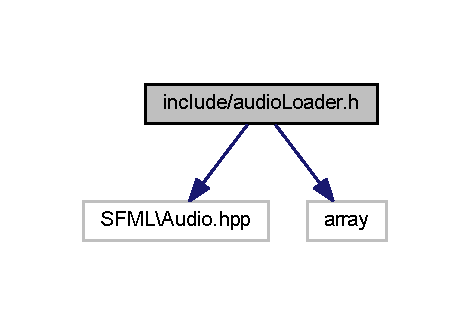
\includegraphics[width=226pt]{audio_loader_8h__incl}
\end{center}
\end{figure}
This graph shows which files directly or indirectly include this file\+:\nopagebreak
\begin{figure}[H]
\begin{center}
\leavevmode
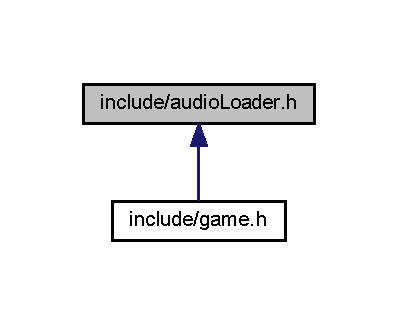
\includegraphics[width=191pt]{audio_loader_8h__dep__incl}
\end{center}
\end{figure}
\subsection*{Classes}
\begin{DoxyCompactItemize}
\item 
class \hyperlink{class_audio_loader}{Audio\+Loader}
\begin{DoxyCompactList}\small\item\em This class is used to manage audio. \end{DoxyCompactList}\end{DoxyCompactItemize}

\hypertarget{checkpoint_8h}{}\section{include/checkpoint.h File Reference}
\label{checkpoint_8h}\index{include/checkpoint.\+h@{include/checkpoint.\+h}}
{\ttfamily \#include \char`\"{}rectangle.\+h\char`\"{}}\\*
Include dependency graph for checkpoint.\+h\+:\nopagebreak
\begin{figure}[H]
\begin{center}
\leavevmode
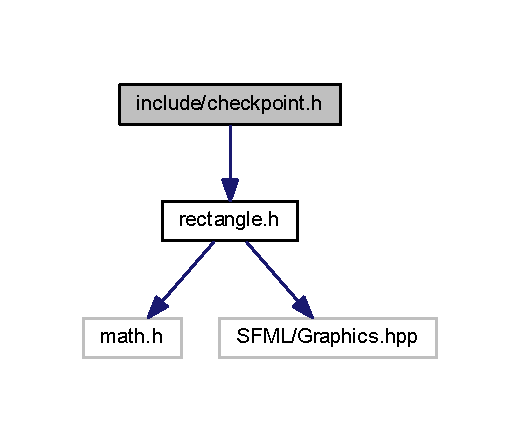
\includegraphics[width=250pt]{checkpoint_8h__incl}
\end{center}
\end{figure}
This graph shows which files directly or indirectly include this file\+:\nopagebreak
\begin{figure}[H]
\begin{center}
\leavevmode
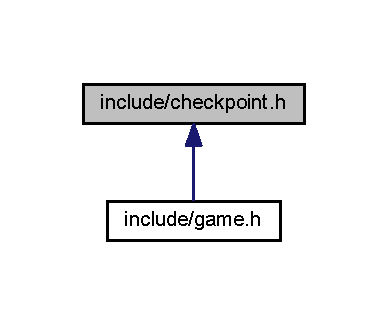
\includegraphics[width=186pt]{checkpoint_8h__dep__incl}
\end{center}
\end{figure}
\subsection*{Classes}
\begin{DoxyCompactItemize}
\item 
class \hyperlink{class_checkpoint}{Checkpoint}
\begin{DoxyCompactList}\small\item\em This class is used to do create a simple checkpoint. \end{DoxyCompactList}\end{DoxyCompactItemize}

\hypertarget{circle_8h}{}\section{include/circle.h File Reference}
\label{circle_8h}\index{include/circle.\+h@{include/circle.\+h}}
{\ttfamily \#include $<$S\+F\+M\+L/\+Graphics.\+hpp$>$}\\*
Include dependency graph for circle.\+h\+:\nopagebreak
\begin{figure}[H]
\begin{center}
\leavevmode
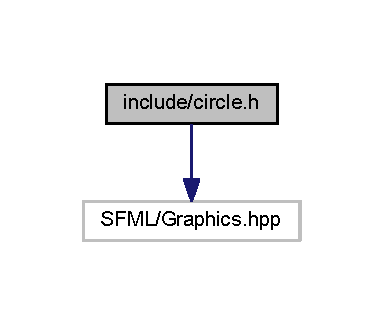
\includegraphics[width=184pt]{circle_8h__incl}
\end{center}
\end{figure}
This graph shows which files directly or indirectly include this file\+:\nopagebreak
\begin{figure}[H]
\begin{center}
\leavevmode
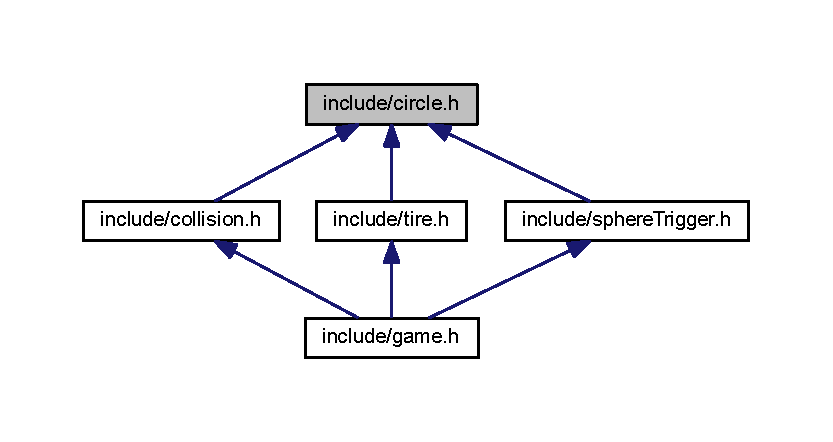
\includegraphics[width=350pt]{circle_8h__dep__incl}
\end{center}
\end{figure}
\subsection*{Classes}
\begin{DoxyCompactItemize}
\item 
class \hyperlink{class_circle}{Circle}
\begin{DoxyCompactList}\small\item\em This class is used to create an abstract base class of the circle. \end{DoxyCompactList}\end{DoxyCompactItemize}

\hypertarget{collision_8h}{}\section{include/collision.h File Reference}
\label{collision_8h}\index{include/collision.\+h@{include/collision.\+h}}
{\ttfamily \#include \char`\"{}rectangle.\+h\char`\"{}}\\*
{\ttfamily \#include \char`\"{}circle.\+h\char`\"{}}\\*
{\ttfamily \#include \char`\"{}vector\+Maths.\+h\char`\"{}}\\*
Include dependency graph for collision.\+h\+:\nopagebreak
\begin{figure}[H]
\begin{center}
\leavevmode
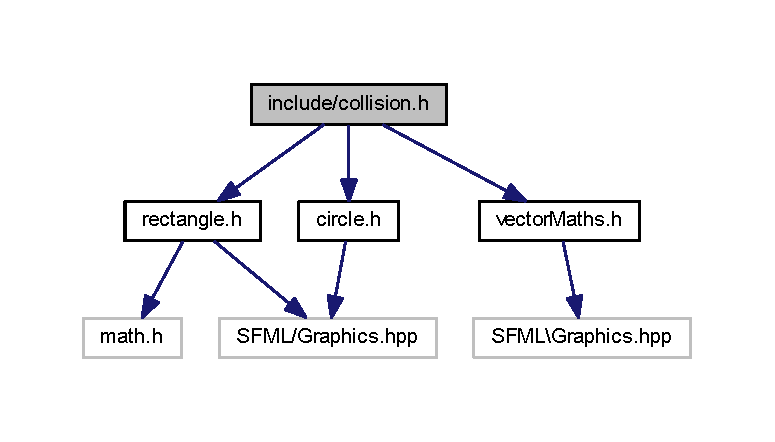
\includegraphics[width=350pt]{collision_8h__incl}
\end{center}
\end{figure}
This graph shows which files directly or indirectly include this file\+:\nopagebreak
\begin{figure}[H]
\begin{center}
\leavevmode
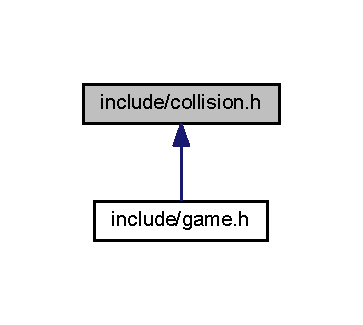
\includegraphics[width=174pt]{collision_8h__dep__incl}
\end{center}
\end{figure}
\subsection*{Classes}
\begin{DoxyCompactItemize}
\item 
class \hyperlink{class_collision}{Collision}
\begin{DoxyCompactList}\small\item\em This class is used to do collision tests. \end{DoxyCompactList}\end{DoxyCompactItemize}

\hypertarget{font_loader_8h}{}\section{include/font\+Loader.h File Reference}
\label{font_loader_8h}\index{include/font\+Loader.\+h@{include/font\+Loader.\+h}}
{\ttfamily \#include $<$S\+F\+M\+L\textbackslash{}\+Graphics.\+hpp$>$}\\*
Include dependency graph for font\+Loader.\+h\+:\nopagebreak
\begin{figure}[H]
\begin{center}
\leavevmode
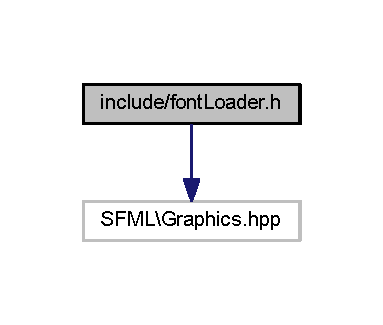
\includegraphics[width=184pt]{font_loader_8h__incl}
\end{center}
\end{figure}
This graph shows which files directly or indirectly include this file\+:\nopagebreak
\begin{figure}[H]
\begin{center}
\leavevmode
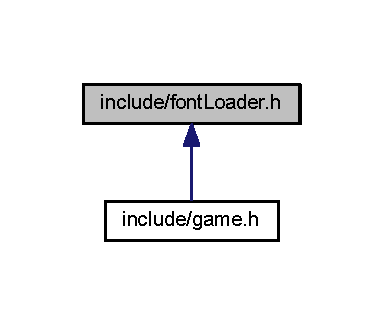
\includegraphics[width=184pt]{font_loader_8h__dep__incl}
\end{center}
\end{figure}
\subsection*{Classes}
\begin{DoxyCompactItemize}
\item 
class \hyperlink{class_font_loader}{Font\+Loader}
\begin{DoxyCompactList}\small\item\em This class is used to manage fonts. \end{DoxyCompactList}\end{DoxyCompactItemize}

\hypertarget{game_8h}{}\section{include/game.h File Reference}
\label{game_8h}\index{include/game.\+h@{include/game.\+h}}
{\ttfamily \#include $<$S\+F\+M\+L/\+Graphics.\+hpp$>$}\\*
{\ttfamily \#include $<$iostream$>$}\\*
{\ttfamily \#include $<$array$>$}\\*
{\ttfamily \#include $<$sstream$>$}\\*
{\ttfamily \#include \char`\"{}player.\+h\char`\"{}}\\*
{\ttfamily \#include \char`\"{}wall.\+h\char`\"{}}\\*
{\ttfamily \#include \char`\"{}image.\+h\char`\"{}}\\*
{\ttfamily \#include \char`\"{}collision.\+h\char`\"{}}\\*
{\ttfamily \#include \char`\"{}view.\+h\char`\"{}}\\*
{\ttfamily \#include \char`\"{}texture\+Loader.\+h\char`\"{}}\\*
{\ttfamily \#include \char`\"{}font\+Loader.\+h\char`\"{}}\\*
{\ttfamily \#include \char`\"{}audio\+Loader.\+h\char`\"{}}\\*
{\ttfamily \#include \char`\"{}simple\+Text.\+h\char`\"{}}\\*
{\ttfamily \#include \char`\"{}tire.\+h\char`\"{}}\\*
{\ttfamily \#include \char`\"{}vector\+Maths.\+h\char`\"{}}\\*
{\ttfamily \#include \char`\"{}sphere\+Trigger.\+h\char`\"{}}\\*
{\ttfamily \#include \char`\"{}rectangle\+Trigger.\+h\char`\"{}}\\*
{\ttfamily \#include \char`\"{}checkpoint.\+h\char`\"{}}\\*
{\ttfamily \#include \char`\"{}static\+Car.\+h\char`\"{}}\\*
Include dependency graph for game.\+h\+:\nopagebreak
\begin{figure}[H]
\begin{center}
\leavevmode
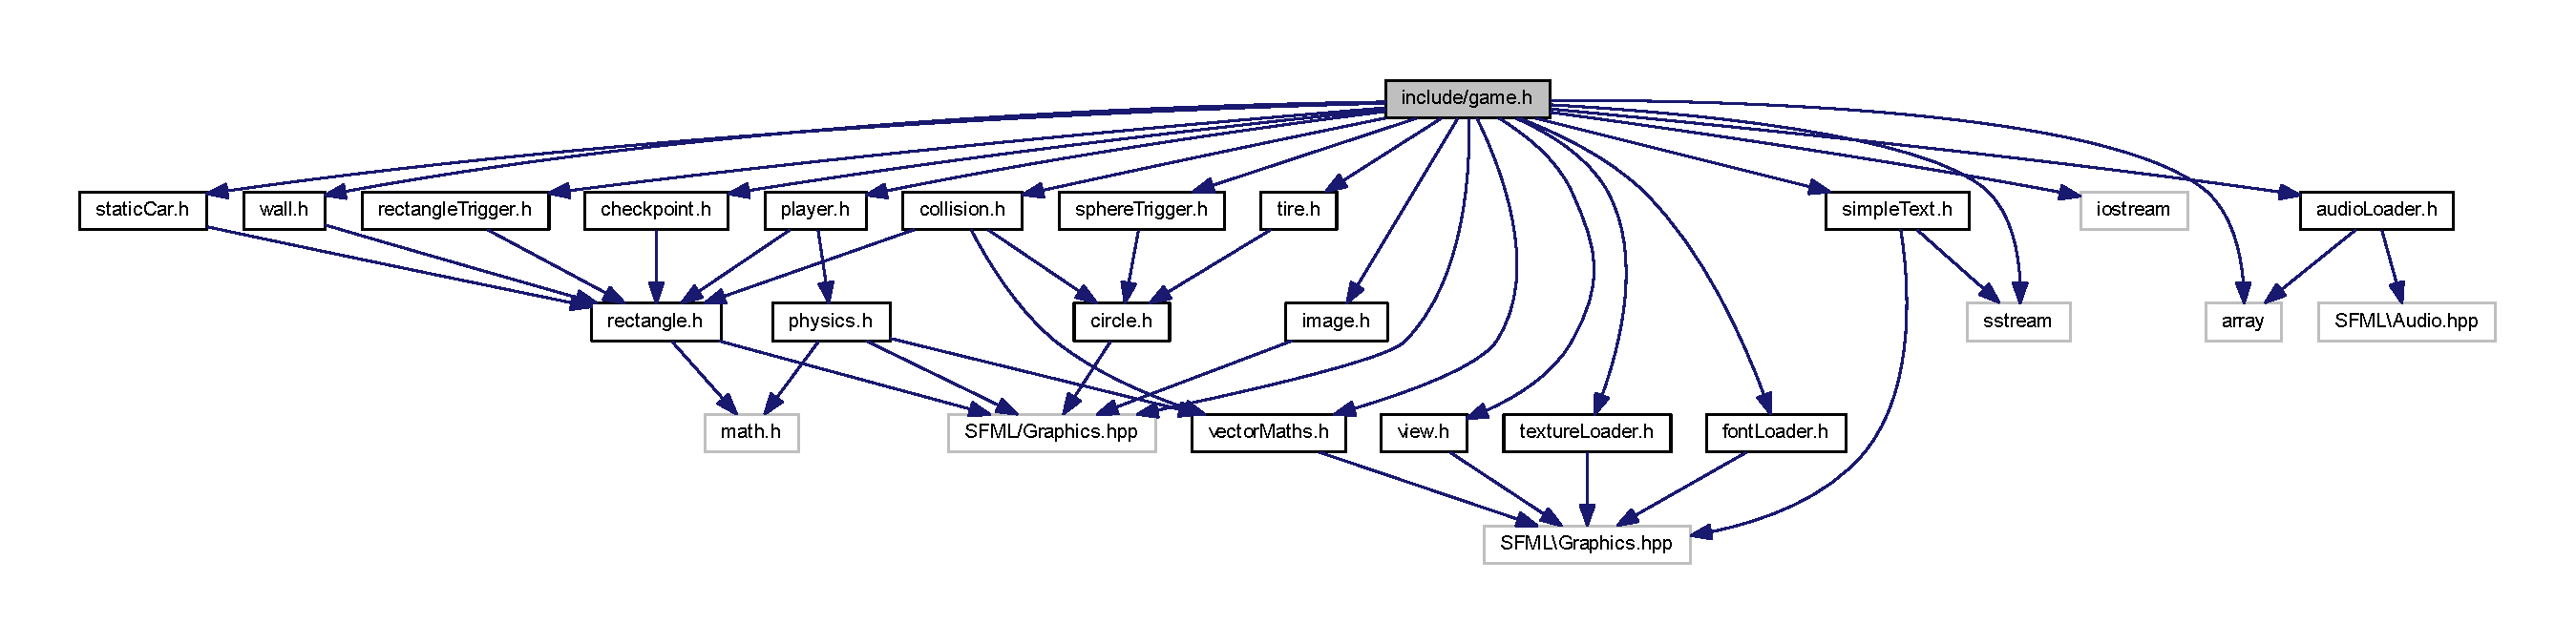
\includegraphics[width=350pt]{game_8h__incl}
\end{center}
\end{figure}
\subsection*{Classes}
\begin{DoxyCompactItemize}
\item 
class \hyperlink{class_game}{Game}
\begin{DoxyCompactList}\small\item\em This class is used to create a game window. \end{DoxyCompactList}\end{DoxyCompactItemize}

\hypertarget{image_8h}{}\section{include/image.h File Reference}
\label{image_8h}\index{include/image.\+h@{include/image.\+h}}
{\ttfamily \#include $<$S\+F\+M\+L/\+Graphics.\+hpp$>$}\\*
Include dependency graph for image.\+h\+:\nopagebreak
\begin{figure}[H]
\begin{center}
\leavevmode
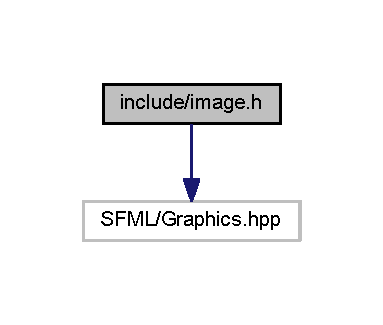
\includegraphics[width=184pt]{image_8h__incl}
\end{center}
\end{figure}
This graph shows which files directly or indirectly include this file\+:\nopagebreak
\begin{figure}[H]
\begin{center}
\leavevmode
\includegraphics[width=165pt]{image_8h__dep__incl}
\end{center}
\end{figure}
\subsection*{Classes}
\begin{DoxyCompactItemize}
\item 
class \hyperlink{class_image}{Image}
\begin{DoxyCompactList}\small\item\em This class is used to construct an image. \end{DoxyCompactList}\end{DoxyCompactItemize}

\hypertarget{physics_8h}{}\section{include/physics.h File Reference}
\label{physics_8h}\index{include/physics.\+h@{include/physics.\+h}}
{\ttfamily \#include $<$S\+F\+M\+L/\+Graphics.\+hpp$>$}\\*
{\ttfamily \#include $<$math.\+h$>$}\\*
{\ttfamily \#include \char`\"{}vector\+Maths.\+h\char`\"{}}\\*
Include dependency graph for physics.\+h\+:\nopagebreak
\begin{figure}[H]
\begin{center}
\leavevmode
\includegraphics[width=350pt]{physics_8h__incl}
\end{center}
\end{figure}
This graph shows which files directly or indirectly include this file\+:\nopagebreak
\begin{figure}[H]
\begin{center}
\leavevmode
\includegraphics[width=172pt]{physics_8h__dep__incl}
\end{center}
\end{figure}
\subsection*{Classes}
\begin{DoxyCompactItemize}
\item 
class \hyperlink{class_physics}{Physics}
\begin{DoxyCompactList}\small\item\em This class is used to create a simulation of movement. \end{DoxyCompactList}\end{DoxyCompactItemize}
\subsection*{Macros}
\begin{DoxyCompactItemize}
\item 
\#define \hyperlink{physics_8h_a525335710b53cb064ca56b936120431e}{\+\_\+\+U\+S\+E\+\_\+\+M\+A\+T\+H\+\_\+\+D\+E\+F\+I\+N\+ES}
\end{DoxyCompactItemize}


\subsection{Macro Definition Documentation}
\index{physics.\+h@{physics.\+h}!\+\_\+\+U\+S\+E\+\_\+\+M\+A\+T\+H\+\_\+\+D\+E\+F\+I\+N\+ES@{\+\_\+\+U\+S\+E\+\_\+\+M\+A\+T\+H\+\_\+\+D\+E\+F\+I\+N\+ES}}
\index{\+\_\+\+U\+S\+E\+\_\+\+M\+A\+T\+H\+\_\+\+D\+E\+F\+I\+N\+ES@{\+\_\+\+U\+S\+E\+\_\+\+M\+A\+T\+H\+\_\+\+D\+E\+F\+I\+N\+ES}!physics.\+h@{physics.\+h}}
\subsubsection[{\texorpdfstring{\+\_\+\+U\+S\+E\+\_\+\+M\+A\+T\+H\+\_\+\+D\+E\+F\+I\+N\+ES}{_USE_MATH_DEFINES}}]{\setlength{\rightskip}{0pt plus 5cm}\#define \+\_\+\+U\+S\+E\+\_\+\+M\+A\+T\+H\+\_\+\+D\+E\+F\+I\+N\+ES}\hypertarget{physics_8h_a525335710b53cb064ca56b936120431e}{}\label{physics_8h_a525335710b53cb064ca56b936120431e}

\hypertarget{player_8h}{}\section{include/player.h File Reference}
\label{player_8h}\index{include/player.\+h@{include/player.\+h}}
{\ttfamily \#include \char`\"{}rectangle.\+h\char`\"{}}\\*
{\ttfamily \#include \char`\"{}physics.\+h\char`\"{}}\\*
Include dependency graph for player.\+h\+:\nopagebreak
\begin{figure}[H]
\begin{center}
\leavevmode
\includegraphics[width=350pt]{player_8h__incl}
\end{center}
\end{figure}
This graph shows which files directly or indirectly include this file\+:\nopagebreak
\begin{figure}[H]
\begin{center}
\leavevmode
\includegraphics[width=165pt]{player_8h__dep__incl}
\end{center}
\end{figure}
\subsection*{Classes}
\begin{DoxyCompactItemize}
\item 
class \hyperlink{class_player}{Player}
\begin{DoxyCompactList}\small\item\em This class is used to create and control a player. \end{DoxyCompactList}\end{DoxyCompactItemize}

\hypertarget{rectangle_8h}{}\section{include/rectangle.h File Reference}
\label{rectangle_8h}\index{include/rectangle.\+h@{include/rectangle.\+h}}
{\ttfamily \#include $<$math.\+h$>$}\\*
{\ttfamily \#include $<$S\+F\+M\+L/\+Graphics.\+hpp$>$}\\*
Include dependency graph for rectangle.\+h\+:\nopagebreak
\begin{figure}[H]
\begin{center}
\leavevmode
\includegraphics[width=250pt]{rectangle_8h__incl}
\end{center}
\end{figure}
This graph shows which files directly or indirectly include this file\+:\nopagebreak
\begin{figure}[H]
\begin{center}
\leavevmode
\includegraphics[width=350pt]{rectangle_8h__dep__incl}
\end{center}
\end{figure}
\subsection*{Classes}
\begin{DoxyCompactItemize}
\item 
class \hyperlink{class_rectangle}{Rectangle}
\begin{DoxyCompactList}\small\item\em This class is used to create an abstract base class of the rectangle. \end{DoxyCompactList}\end{DoxyCompactItemize}
\subsection*{Macros}
\begin{DoxyCompactItemize}
\item 
\#define \hyperlink{rectangle_8h_a525335710b53cb064ca56b936120431e}{\+\_\+\+U\+S\+E\+\_\+\+M\+A\+T\+H\+\_\+\+D\+E\+F\+I\+N\+ES}
\end{DoxyCompactItemize}


\subsection{Macro Definition Documentation}
\index{rectangle.\+h@{rectangle.\+h}!\+\_\+\+U\+S\+E\+\_\+\+M\+A\+T\+H\+\_\+\+D\+E\+F\+I\+N\+ES@{\+\_\+\+U\+S\+E\+\_\+\+M\+A\+T\+H\+\_\+\+D\+E\+F\+I\+N\+ES}}
\index{\+\_\+\+U\+S\+E\+\_\+\+M\+A\+T\+H\+\_\+\+D\+E\+F\+I\+N\+ES@{\+\_\+\+U\+S\+E\+\_\+\+M\+A\+T\+H\+\_\+\+D\+E\+F\+I\+N\+ES}!rectangle.\+h@{rectangle.\+h}}
\subsubsection[{\texorpdfstring{\+\_\+\+U\+S\+E\+\_\+\+M\+A\+T\+H\+\_\+\+D\+E\+F\+I\+N\+ES}{_USE_MATH_DEFINES}}]{\setlength{\rightskip}{0pt plus 5cm}\#define \+\_\+\+U\+S\+E\+\_\+\+M\+A\+T\+H\+\_\+\+D\+E\+F\+I\+N\+ES}\hypertarget{rectangle_8h_a525335710b53cb064ca56b936120431e}{}\label{rectangle_8h_a525335710b53cb064ca56b936120431e}

\hypertarget{rectangle_trigger_8h}{}\section{include/rectangle\+Trigger.h File Reference}
\label{rectangle_trigger_8h}\index{include/rectangle\+Trigger.\+h@{include/rectangle\+Trigger.\+h}}
{\ttfamily \#include \char`\"{}rectangle.\+h\char`\"{}}\\*
Include dependency graph for rectangle\+Trigger.\+h\+:\nopagebreak
\begin{figure}[H]
\begin{center}
\leavevmode
\includegraphics[width=250pt]{rectangle_trigger_8h__incl}
\end{center}
\end{figure}
This graph shows which files directly or indirectly include this file\+:\nopagebreak
\begin{figure}[H]
\begin{center}
\leavevmode
\includegraphics[width=208pt]{rectangle_trigger_8h__dep__incl}
\end{center}
\end{figure}
\subsection*{Classes}
\begin{DoxyCompactItemize}
\item 
class \hyperlink{class_rectangle_trigger}{Rectangle\+Trigger}
\begin{DoxyCompactList}\small\item\em This class is used to create a trigger. \end{DoxyCompactList}\end{DoxyCompactItemize}

\hypertarget{simple_text_8h}{}\section{include/simple\+Text.h File Reference}
\label{simple_text_8h}\index{include/simple\+Text.\+h@{include/simple\+Text.\+h}}
{\ttfamily \#include $<$S\+F\+M\+L\textbackslash{}\+Graphics.\+hpp$>$}\\*
{\ttfamily \#include $<$sstream$>$}\\*
Include dependency graph for simple\+Text.\+h\+:\nopagebreak
\begin{figure}[H]
\begin{center}
\leavevmode
\includegraphics[width=254pt]{simple_text_8h__incl}
\end{center}
\end{figure}
This graph shows which files directly or indirectly include this file\+:\nopagebreak
\begin{figure}[H]
\begin{center}
\leavevmode
\includegraphics[width=186pt]{simple_text_8h__dep__incl}
\end{center}
\end{figure}
\subsection*{Classes}
\begin{DoxyCompactItemize}
\item 
class \hyperlink{class_simple_text}{Simple\+Text}
\begin{DoxyCompactList}\small\item\em This class is used to create a simple text on the screen. \end{DoxyCompactList}\end{DoxyCompactItemize}

\hypertarget{sphere_trigger_8h}{}\section{include/sphere\+Trigger.h File Reference}
\label{sphere_trigger_8h}\index{include/sphere\+Trigger.\+h@{include/sphere\+Trigger.\+h}}
{\ttfamily \#include \char`\"{}circle.\+h\char`\"{}}\\*
Include dependency graph for sphere\+Trigger.\+h\+:\nopagebreak
\begin{figure}[H]
\begin{center}
\leavevmode
\includegraphics[width=197pt]{sphere_trigger_8h__incl}
\end{center}
\end{figure}
This graph shows which files directly or indirectly include this file\+:\nopagebreak
\begin{figure}[H]
\begin{center}
\leavevmode
\includegraphics[width=197pt]{sphere_trigger_8h__dep__incl}
\end{center}
\end{figure}
\subsection*{Classes}
\begin{DoxyCompactItemize}
\item 
class \hyperlink{class_sphere_trigger}{Sphere\+Trigger}
\begin{DoxyCompactList}\small\item\em This class is used to create a trigger. \end{DoxyCompactList}\end{DoxyCompactItemize}

\hypertarget{static_car_8h}{}\section{include/static\+Car.h File Reference}
\label{static_car_8h}\index{include/static\+Car.\+h@{include/static\+Car.\+h}}
{\ttfamily \#include \char`\"{}rectangle.\+h\char`\"{}}\\*
Include dependency graph for static\+Car.\+h\+:\nopagebreak
\begin{figure}[H]
\begin{center}
\leavevmode
\includegraphics[width=250pt]{static_car_8h__incl}
\end{center}
\end{figure}
This graph shows which files directly or indirectly include this file\+:\nopagebreak
\begin{figure}[H]
\begin{center}
\leavevmode
\includegraphics[width=178pt]{static_car_8h__dep__incl}
\end{center}
\end{figure}
\subsection*{Classes}
\begin{DoxyCompactItemize}
\item 
class \hyperlink{class_static_car}{Static\+Car}
\begin{DoxyCompactList}\small\item\em This class is used to create immovable cars. \end{DoxyCompactList}\end{DoxyCompactItemize}

\hypertarget{texture_loader_8h}{}\section{include/texture\+Loader.h File Reference}
\label{texture_loader_8h}\index{include/texture\+Loader.\+h@{include/texture\+Loader.\+h}}
{\ttfamily \#include $<$S\+F\+M\+L\textbackslash{}\+Graphics.\+hpp$>$}\\*
Include dependency graph for texture\+Loader.\+h\+:\nopagebreak
\begin{figure}[H]
\begin{center}
\leavevmode
\includegraphics[width=198pt]{texture_loader_8h__incl}
\end{center}
\end{figure}
This graph shows which files directly or indirectly include this file\+:\nopagebreak
\begin{figure}[H]
\begin{center}
\leavevmode
\includegraphics[width=198pt]{texture_loader_8h__dep__incl}
\end{center}
\end{figure}
\subsection*{Classes}
\begin{DoxyCompactItemize}
\item 
class \hyperlink{class_texture_loader}{Texture\+Loader}
\begin{DoxyCompactList}\small\item\em This class is used to manage textures. \end{DoxyCompactList}\end{DoxyCompactItemize}

\hypertarget{tire_8h}{}\section{include/tire.h File Reference}
\label{tire_8h}\index{include/tire.\+h@{include/tire.\+h}}
{\ttfamily \#include \char`\"{}circle.\+h\char`\"{}}\\*
Include dependency graph for tire.\+h\+:\nopagebreak
\begin{figure}[H]
\begin{center}
\leavevmode
\includegraphics[width=184pt]{tire_8h__incl}
\end{center}
\end{figure}
This graph shows which files directly or indirectly include this file\+:\nopagebreak
\begin{figure}[H]
\begin{center}
\leavevmode
\includegraphics[width=163pt]{tire_8h__dep__incl}
\end{center}
\end{figure}
\subsection*{Classes}
\begin{DoxyCompactItemize}
\item 
class \hyperlink{class_tire}{Tire}
\begin{DoxyCompactList}\small\item\em This class is used to construct a tire. \end{DoxyCompactList}\end{DoxyCompactItemize}

\hypertarget{vector_maths_8h}{}\section{include/vector\+Maths.h File Reference}
\label{vector_maths_8h}\index{include/vector\+Maths.\+h@{include/vector\+Maths.\+h}}
{\ttfamily \#include $<$S\+F\+M\+L\textbackslash{}\+Graphics.\+hpp$>$}\\*
Include dependency graph for vector\+Maths.\+h\+:\nopagebreak
\begin{figure}[H]
\begin{center}
\leavevmode
\includegraphics[width=191pt]{vector_maths_8h__incl}
\end{center}
\end{figure}
This graph shows which files directly or indirectly include this file\+:\nopagebreak
\begin{figure}[H]
\begin{center}
\leavevmode
\includegraphics[width=322pt]{vector_maths_8h__dep__incl}
\end{center}
\end{figure}
\subsection*{Classes}
\begin{DoxyCompactItemize}
\item 
class \hyperlink{class_vector_maths}{Vector\+Maths}
\begin{DoxyCompactList}\small\item\em This class is used to do simple vector calculations. \end{DoxyCompactList}\end{DoxyCompactItemize}

\hypertarget{view_8h}{}\section{include/view.h File Reference}
\label{view_8h}\index{include/view.\+h@{include/view.\+h}}
{\ttfamily \#include $<$S\+F\+M\+L\textbackslash{}\+Graphics.\+hpp$>$}\\*
Include dependency graph for view.\+h\+:\nopagebreak
\begin{figure}[H]
\begin{center}
\leavevmode
\includegraphics[width=184pt]{view_8h__incl}
\end{center}
\end{figure}
This graph shows which files directly or indirectly include this file\+:\nopagebreak
\begin{figure}[H]
\begin{center}
\leavevmode
\includegraphics[width=163pt]{view_8h__dep__incl}
\end{center}
\end{figure}
\subsection*{Classes}
\begin{DoxyCompactItemize}
\item 
class \hyperlink{class_view}{View}
\begin{DoxyCompactList}\small\item\em This class is used to manage a scene. \end{DoxyCompactList}\end{DoxyCompactItemize}

\hypertarget{wall_8h}{}\section{include/wall.h File Reference}
\label{wall_8h}\index{include/wall.\+h@{include/wall.\+h}}
{\ttfamily \#include \char`\"{}rectangle.\+h\char`\"{}}\\*
Include dependency graph for wall.\+h\+:\nopagebreak
\begin{figure}[H]
\begin{center}
\leavevmode
\includegraphics[width=250pt]{wall_8h__incl}
\end{center}
\end{figure}
This graph shows which files directly or indirectly include this file\+:\nopagebreak
\begin{figure}[H]
\begin{center}
\leavevmode
\includegraphics[width=163pt]{wall_8h__dep__incl}
\end{center}
\end{figure}
\subsection*{Classes}
\begin{DoxyCompactItemize}
\item 
class \hyperlink{class_wall}{Wall}
\begin{DoxyCompactList}\small\item\em This class is used to construct a wall. \end{DoxyCompactList}\end{DoxyCompactItemize}

%--- End generated contents ---

% Index
\backmatter
\newpage
\phantomsection
\clearemptydoublepage
\addcontentsline{toc}{chapter}{Index}
\printindex

\end{document}
